\chapter{Polarized $^{3}$He for Neutron Spin Analysis}
\label{ch:polHe}

\ifpdf
    \graphicspath{{Chapter2/Figs/Raster/}{Chapter2/Figs/PDF/}{Chapter2/Figs/}}
\else
    \graphicspath{{Chapter2/Figs/Vector/}{Chapter2/Figs/}}
\fi

This chapter describes the in situ (at the experiment location) $^3$He SEOP polarization setup used for the neutron polarization and transmission measurements at the SNS Beamline 13A. First, the methodology to polarize $^{3}$He is described, then the design of the in situ system along with the results from proof of demonstration are shown and discussed.

\section{Polarized $^{3}$He}

Targets of gaseous spin polarized $^3$He nuclei are widely used in nuclear physics as polarized “free neutrons” for electron scattering experiments and as spin filters/analyzers of polarized neutron beams due to the large spin dependent absorption cross section of neutrons by $^3$He \cite{Gentile2017}. Convenience of long polarization relaxation times ($\sim 10^2$ hours) due to the noble gas chemical inertness, absence of an electric quadrupole moment and the presence of a large magnetic moment make $^3$He attractive for precision measurements. This utility is enabled by methods used to hyperpolarize $^3$He atoms. 

It is not possible to directly polarize the $^3$He 1s$^2$-1s2p transition since the hyperfine splitting in 1s2p state is very small, resulting in mixing of the hyperfine levels of the excited state, not to mention, the lack of 59nm (extreme UV) laser technology \footnote{Technically, one can use a Stern-Gerlach filter or the Lamb shift transitions in the small Zeeman splitting of the 2s[F=1/2] states in $^3$He to polarize $^3$He \cite{Schieck2011}.} \cite{Schieck2011}. Thus spin exchange (SEOP) and metastability exchange (MEOP) optical pumping methods involving indirect transfer of angular momentum are used \cite{Gentile2017}. In SEOP, alkali atoms at $\sim$bar pressure are polarized via optical pumping of their electronic structure \cite{Walker1997}. Transfer of angular momentum from alkali to He occurs via slow and weak Hyperfine interactions \cite{Walker1997}. In MEOP, metastable $^3$He atoms are created via optical pumping and are rapidly polarized via weak Hyperfine mixing \cite{Batz2011}. The polarized metastable $^3$He atoms are transferred to the polarized ground state $^3$He via exchange collisions \cite{Batz2011}. This section gives a brief overview of the two optical pumping methods to provide context for this thesis. A more comprehensive overview can be found in \cite{Gentile2017}.

\subsection{Spin Exchange Optical Pumping}

%In SEOP, alkali atoms are polarized via optical pumping of their electronic structure. Transfer of angular momentum from alkali to $^3$He transpires via slow and weak Hyperfine interactions \cite{Bouchiat1960,Walker1997}. 

The first demonstration of SEOP on $^3$He was done by \cite{Bouchiat1960} in 1960. With the advancement in laser technology, \cite{Chupp1987} used laser based SEOP to develop high density polarized $^3$He for discriminating neutron polarization. Even today, the laser based SEOP is the most widely used technique to perform SEOP.

Glass cells filled with 0.1 to 10 bar\footnote{All pressures listed in this section are at standard temperatures unless otherwise stated.} pressure of ultra-high purity (99.999\%) $^3$He gas along with $\sim$100mg of Rubidium and Potassium alkali metal mixture are used for confining and polarizing $^3$He. The cells are heated to 190~\degree C to 210~\degree C to vaporize the alkali mixture to achieve a density of around $10^{14}-10^{15}$ cm$^{-3}$. The entire cell is illuminated with circularly polarized infrared light using a diode laser. The laser output is typically set to 50 W to 100 W power and 795 nm or 770 nm wavelength, which correspond to the D1 transition lines of Rb and K, respectively, with a linewidth of about 0.2 nm \cite{Gentile2017, Ben-AmarBaranga1998, Chen2014}. The alkali density in cells is low enough that the spectral width of the laser is enough to cover the atomic line width broadening from relatively high pressure nature of the cell \cite{Romalis1997, Kluttz2013}. Even though a high degree of circular polarization can be attained with commercial polarizing wave plates \cite{Bhaskar1979, Chann2002}. A small amount of nitrogen gas is also added to quench the radiative decay of the excited alkali atoms \cite{Walker1997, Lancor2010}.

The build up of alkali polarization is determined by a large alkali polarization optical pumping rate as compared to the alkali polarization relaxation rate \cite{Gentile2017}. The alkali spin-relaxation times are on the order of a few ms, whereas the alkali optical pumping times are much shorter, typically $\lesssim$ ms, hence high alkali polarization is established relatively quickly \cite{Chen2011}. These short optical pumping times are possible because of the use of laser based optical pumping as well as keeping the cell at a high temperature to vaporize the optically thick alkali mixture \cite{Gentile2017, Chen2011, Babcock2016}. The alkali spin relaxation is primarily caused by alkali-alkali collisions and alkali-$^3$He collisions \cite{Ben-AmarBaranga1998}. This relaxation due to collisions is highly dependent upon the pressure of $^3$He gas and amount of alkali mixture used during formation of the $^3$He cell \cite{Ben-AmarBaranga1998}. A hybrid mixture of K and Rb alkali atoms is used due to their high spin exchange efficiency and low spin relaxation rates \cite{Babcock2003, Chen2007}.

Similarly, the build up of $^3$He polarization is determined by a large alkali-$^3$He spin-exchange rate as compared to the $^3$He nuclear spin relaxation \cite{Gentile2017}. The alkali-$^3$He spin exchange time is typically on the order of 10 hours, hence, it takes a day(s) to approach the maximum attainable $^3$He polarization \cite{Chen2011, Gentile2017}. Due to these slow polarization times, it is critical to have long $^3$He polarization relaxation times for a cell in order to maximize its use. GE180, a type of Aluminosilicate glass, which has low $^3$He permeability, is boron free and corrosion resistant, is widely used for neutron based experiments \cite{Newbury1993, Chen2014, Heil1995}. Polarized $^3$He cells at room temperature have shown relaxation times on the order of 100 hours  \cite{Chen2011}. This indicates that relaxation due to glass cell wall has a minor contribution towards limiting the attainable $^3$He polarization. However, relaxation from temperature effects has been found to restrict the $^3$He polarization \cite{Babcock2006}. These main limiting effects will be discussed later in this chapter.

In a typical SEOP apparatus, an oven is used to heat the glass cell filled with of alkali mixture and $^3$He \cite{Tong2010, Babcock2016}, a magnetic field coil to provide uniform holding magnetic field, a high-power laser with narrow spectral width \cite{Babcock2005, Chen2014, Liu2015} and laser optics for generating circularly polarized light and steering/focusing the laser beam. $^3$He polarization is monitored and controlled using nuclear magnetic resonance (NMR) techniques as well as alkali spectroscopy \cite{Romalis1998}.


\subsection{Metastability Exchange Optical Pumping}

In MEOP, $^3$He is polarized via optical pumping and hyperfine interactions of metastable $^3$He atoms followed by rapid transitions to the ground state via metastable state to ground state exchange collisions \cite{Colegrove1963, Batz2011}.  MEOP is usually performed on $^3$He cells with pressures on the order of $\sim$mbar. External electrodes are used to produce a RF discharge to make metastable atoms on the order of $10^{10}$ cm$^{-3}$ \cite{Colegrove1963, Batz2011, Gentile2017}. Ionization of impurities can lead to destruction of metastability, so ultra-high purity gases and clean glass cells are used. The low density of $^3$He means low density of metastable states, hence, larger cells are used to absorb the optical pumping light to overcome the optically thin nature and  yield larger quantities of polarized $^3$He. Optical pumping is performed via $\sim$10W lasers at the 1083nm wavelength with spectral linewidth of 15 cm \cite{Colegrove1963, Batz2011, Gentile2017}. This linewidth is much wider than the Doppler-broadened atomic absorption \cite{Colegrove1963, Batz2011, Gentile2017}. The polarization of the $^3$He ground state and metastable $^3$He states are strongly coupled due to the hyperfine interactions \cite{Gentile2017}, and subsequently evolve on the timescale of seconds \cite{Gentile1993}. The $^3$He ground-state relaxation is dependent on the strength of the RF discharges, where strong discharges produce higher densities of metastable states and thus, higher polarization, however, at the expense of large metastability induced relaxations \cite{Batz2011, Gentile2017}. 

The apparatus used to perform MEOP consists of RF discharge electrodes wrapped around the $^3$He cell. The cells resides in a homogeneous magnetic field, which is provided by a large set of coils. The cell is illuminated with a laser outputting circularly polarized IR light \cite{Andersen2005}. During optical pumping, compressors are also used to maintain the $^3$He polarization \cite{Andersen2005}. After compression, NMR is used to monitor/manipulate the $^3$He polarization \cite{Romalis1998}.

\subsection{Comparison of SEOP and MEOP}

Although both SEOP and MEOP can be used to produce polarized $^3$He, the application has to be considered in order to select the appropriate method. The benefit of SEOP is enabling of means to polarize from 0.3 bars to 10 bars pressure $^3$He cells \cite{Gentile2017}. By contrast, MEOP is best deployed for $\sim$1 mbar pressures, requiring further gas compression to preserve the polarization \cite{Gentile2017}. The advantage of MEOP is the ability to polarize $^3$He at timescales faster (typically seconds) than most SEOP (typically hours) \cite{Gentile2017}.  In terms of operations, SEOP can be done in compact setups without the need for supervision during the hours long build up towards polarization \cite{Jiang2013}, while MEOP requires large laboratory space to accommodate the bulky setup as well as live supervision to operate the gas compression, albeit for short times \cite{Batz2011}. For neutron applications, such as the experiment described in this thesis, a 0.8bar $^3$He cell was used in a compact in situ apparatus, therefore SEOP was the suitable method. SEOP has also been the preferred choice for other $^3$He cells/neutron spin fliters used at Oak Ridge National Laboratory, therefore, the presence of technical expertise and pre-existing equipment was beneficial to the work described in this thesis. 

\section{Theory of Spin Exchange Optical Pumping}

\subsection{Optical Pumping}

As stated earlier in this chapter, the SEOP process facilitates the polarization of $^3$He by polarized alkali atoms, therefore, it is necessary to optically pump and polarize the alkali with high efficiency. This optical pumping is performed using monochromatic high powered lasers with sharp spectral widths to initiate the hyperfine atomic transitions of the alkali atoms. This section describes the physics of alkali optical pumping, the causes of alkali spin relaxation as well the circularly polarized light dependent effects on the efficiency of optical pumping. A detailed explanation of the optical pumping mechanism can be found in \cite{Gentile2017, Happer1987, Walker2011}. The SEOP mechanism described in this section is adopted from the terminology and nomenclature in \cite{Gentile2017}.

\afterpage{
\begin{figure}
    \centering
    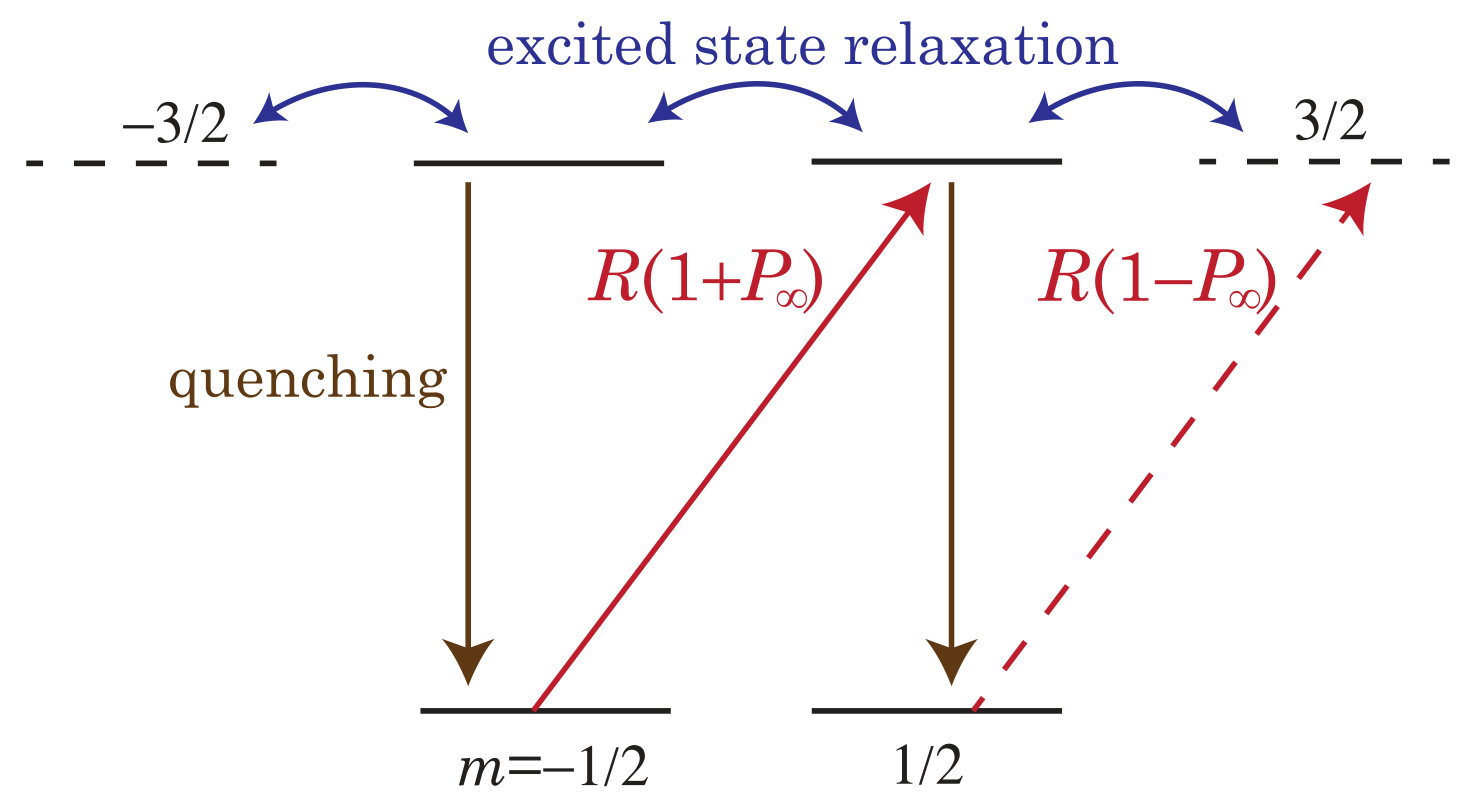
\includegraphics[width=\textwidth]{figures/chapter3-figs/OPalkalistates.png}
    \caption[Hyperfine atomic levels involved in the the optical pumping via light of the alkali $S_{1/2}$ to $P_{1/2}$ D1 resonance in the presence of $^3$He.]
    {Hyperfine atomic levels involved in the the optical pumping of the alkali $S_{1/2}$ to $P_{1/2}$ D1 line in the presence of $^3$He. The $^3$He atoms mix the P-levels of the alkali, modifying the ground state to the excited state selection rules. Alkali in the $m_S= \pm \frac{1}{2}$  ground-state Zeeman sublevels absorb light with $1 \mp P_{\infty}$, probability. Once the alkali transitions to the excited state, spin relaxing collisions can occur. N$_2$ gas is used to quench any alkali radiative and al de-excitations and relaxes the alkali to the ground-state Zeeman sublevels. The alkali, over time, accumulates in the $m_S=\frac{1}{2}$ Zeeman sublevel, acquiring a steady-state hyperfine spin polarization of $P_{\infty}$ assuming that spin relaxation in the alkali ground-state is absent. Figure taken from \cite{Gentile2017}.}
    \label{fig:opticalpumping}
\end{figure}
\clearpage}

A more detailed description of the alkali atomic spectrum especially the D lines of Rb and K can be found in \cite{Steck2023Rb85, Steck2023Rb87, Tiecke2019}. \Cref{fig:opticalpumping} shows the relevant hyperfine levels at play during the optical pumping of alkali atoms. It illustrates the optical pumping mechanism from circularly polarized ($\sigma_+$) light absorption tuned to the ground state $S_{\frac{1}{2}}$ to the excited state $P_{\frac{1}{2}}$ “D1” resonance line of the alkali. The figure also shows the presence of mixing of the $P_{\frac{1}{2}}$ and $P_{\frac{3}{2}}$ Zeeman sublevels due to collisions with $^3$He atoms indicated by the dashed lines. 

As illustrated in \cref{fig:opticalpumping}, the D1 line transition probability, $P_{\infty}$, for alkali atoms in the $m_S=-\frac{1}{2}$ Zeeman sublevel transitioning to the the $m_P=\frac{1}{2}$ level is $1+P_{\infty}$. This transition probability much large than the transition probability of $1-P_{\infty}$ for the alkali in the $m_S=\frac{1}{2}$ Zeeman sublevel \cite{Gentile2017, Happer1987, Lancor2010}. This selective transition is possible due to the mixing from the weak hyperfine interactions under the presence of $^3$He \cite{Gentile2017, Happer1987}. Therefore, the alkali atoms in the $m_S=-\frac{1}{2}$ ground state get preferentially excited to $m_P=\frac{1}{2}$ excited state. The excited alkali atoms undergo relaxation due to collisions with the $^3$He gas and an additional quenching gas, N$_2$. This randomizes the excited alkali atom population among the mixed $P_{\frac{1}{2}}$ and the $P_{\frac{3}{2}}$ Zeeman sublevels. Then, there is resonant transfer of the excited alkali P-state energy to vibrational states of N$_2$. This de-excites the alkali atoms back to the $S_{\frac{1}{2}}$ ground state level. The fraction of alkali atoms that de-excite to the $m_S=\frac{1}{2}$ state do not absorb the polarized light, due to selection rules. While the fraction that de-excite to $m_S=-\frac{1}{2}$ get excited back to P-states and relax until all alkali atoms populate the $m_S=\frac{1}{2}$ state. The process continues until a steady-state polarized alkali population builds up, $P_{\infty}$ \cite{Lancor2010}. N$_2$ plays a key role in this process by quenching the excited alkali atoms to prevent radiative de-excitations \cite{Lancor2010}. The mechanism described is valid for high alkali density cells \cite{Gentile2017, Walker1997, Happer1987}. However, for low alkali density cells, rapid electronic de-excitations cause nuclear spin relaxation via hyperfine couplings, reducing the optical pumping efficiency \cite{Lancor2010}.

The spin-exchange collisions among the alkali-metal atoms themselves are responsible for maintaining the collective angular momentum \cite{Happer1972, Appelt1998}. These collisions conserve the total angular momentum ($F_{A}=I_{A}+S_{A}$) and in combination with the alkali hyperfine coupling, establish a thermal spin equilibrium with the total angular momentum states ($F, m_{F}$) as $\rho \propto \exp \left({\frac{ m_{F}}{k_BT}} \right) $ \cite{Happer1972, Appelt1998}, where $k_B$ is the Boltzmann constant and $T$ is temperature. The alkali-metal electron spin polarization can be defined with this spin-temperature parameter as $P_A = \tanh{\frac{1}{2k_BT}}$. In the mechanism described so far, the alkali nuclear spins have neglected. However, since SEOP $^3$He cells are pumped under the application of low magnetic fields, the total alkali hyperfine structure (with a non-zero alkali nuclear spin) and the total angular momentum states ($F, m_{F}$) with ($2F+1$) multiplicity have to be considered. Pressure broadening of the D1 line leaves the total angular momentum states $m_{F}$ unresolved, therefore, all $m_{F}$ states are optically pumped with the same rate. This means that the presence of alkali nuclear spin creates a “slowing-down” effect on the optical pumping, which can be described as $\frac{\langle F_z \rangle}{\langle S_z \rangle} \approx 2I_A + 1$, where only the two states $F=I_A+\frac{1}{2}, m_F = \pm(I_A+\frac{1}{2})$, give rise to the electron spin polarization \cite{Appelt1998}. 

Based on mechanism described, the optical pumping process can be written via the conservation of the total alkali angular momentum \cite{Gentile2017} as:
\begin{equation}
    \frac{d\langle F_z \rangle}{dt} = \frac{1}{2} \left[ R({\bf x}) (P_{\infty} -P_{A}) - \Gamma_A P_{A}    \right]
\end{equation}
where $\Gamma_A$ is the alkali spin relaxation rate and $R({\bf x})$ is the alkali light absorption rate for an arbitrary location, $\bf x$, in a cell. The steady-state polarization at a local position in the cell becomes:
\begin{equation}
    P_{A}({\bf x}) = P_{\infty} \frac{R({\bf x})}{R({\bf x}) + \Gamma_A}
\end{equation}
The next section describes the effects responsible alkali spin relaxation.

\subsubsection{Alkali Relaxation}

There are three as of yet known processes that are responsible for causing alkali spin polarization relaxation in SEOP cells \cite{Gentile2017}. As will be discussed later, the interaction $V_{rot} \propto \Vec{S} \cdot \Vec{N} $, which comes from the alkali electronic spin $\Vec{S}$ to the rotational angular momentum $\Vec{N}$ of the pseudo-rigid alkali-$^3$He pair \cite{Walker1997}, is one of them. This interaction comes from the spin-orbit fine structure interactions induced by the mixed s-p state caused by collisions \cite{Walker1997}. As will be discussed later, this is the reason why Na or K are the ideal SEOP alkali mediators due to their small fine-structure interaction, as compared to Rb. This collision process has a temperature dependence as T$^4$ as well and becomes more prominent at high temperature SEOP \cite{Ben-AmarBaranga1998}.

Secondly, there is also a small dissipation of spin angular momentum among alkali-alkali collisions, which arise from the spin-axis interaction $ V_{SS} \propto \Vec{S} \cdot \Vec{S}$, \cite{Kadlecek2001} as well as from any formation of triplet or singlet alkali molecules \cite{Kadlecek2001, Kadlecek1998, Erickson2000}. At low magnetic fields, collision rate coefficients have been measured to be $1.0 \times 10^{-18}$ cm$^3$ s$^{-1}$ for K-K collisions and $9.3 \times 10^{-18}$ cm$^3$ s$^{-1}$ for Rb-Rb collisions \cite{Gentile2017}, indicating this effect is more persistent in Rb than K, thus making K more suitable.

The high rate of diffusion of the polarized alkali atoms within the cell volume can lead to alkali spin relaxation as well \cite{Gentile2017}. The alkali polarization diffuses on length scales of cm or less as the polarized optical pumping light propagates and attenuates through the cell. However, a thin region of unpolarized alkali atoms can persist near the cell wall \cite{Wagshul1994, Walker1997, Appelt1998, Nelson2001}. The alkali polarization at a distance $x$ from the cell wall can be estimated as $P_A [1- \exp{\left( \frac{-x}{\lambda} \right)}]$, where the diffusive layer thickness, $\lambda$, is approximated to be around $\sim 60 ~\mu $m \cite{Wagshul1994, Walker1997, Appelt1998, Nelson2001}.

\subsubsection{Light Polarization}

The transmission of light through a cell of unpolarized alkali atoms for a typical optical depth, $D_{opt}$, is $\exp{(-100)}$ \cite{Gentile2017}. This is because the alkali vapor is optically dense. If the cell is full of polarized alkali atoms, the optical depth of circularly polarized light becomes $D_{opt}=D_{opt,0}[1 - (P_{\infty}P_{A})]$, which means that the the circularly polarized light can only penetrate further into the cell if $ 1 - (P_{\infty}P_{A}) \ll 1$ i.e. the alkali atoms become fully polarized ($P_{A}\sim1$) in order to become optically transparent ($P_{\infty}\sim1$) \cite{Gentile2017}. This will only happen if optical pumping light is tuned to the D1 line of the alkali atom.

\afterpage{
\begin{figure}
    \centering
    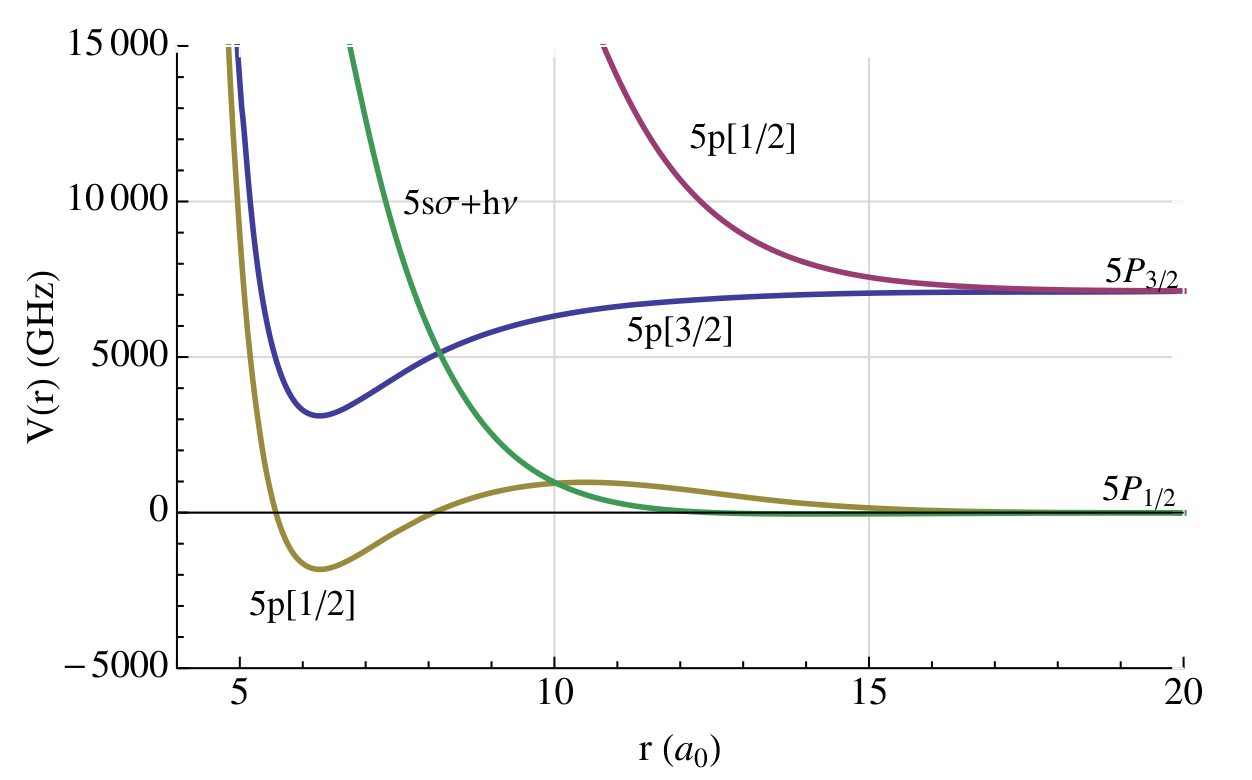
\includegraphics[width=\textwidth]{figures/chapter3-figs/OPalkalimixing.png}
    \caption[Atomic levels of Rb-$^3$He pair during optical pumping.]
    {Atomic levels of Rb-$^3$He pair during optical pumping. The figure shows the absorbtion of the D1 light crossing over with the mixed $5p[\frac{1}{2}]$ excited state. Figure is taken from \cite{Gentile2017} with the original calculations in \cite{Lancor2010}.}
    \label{fig:RbHepumping}
\end{figure}
\clearpage}

Since SEOP is intended for high density $^3$He cells, alkali-$^3$He collisions cause mixing of the alkali D1 atomic levels \cite{Lancor2010}. This is shown in \cref{fig:RbHepumping}. This allows for circularly polarized light to get absorbed in the mixed state, limiting the efficiency of optical pumping \cite{Lancor2010}. Thus, the alkali atoms can only achieve a maximum polarization, $P_{\infty}<1$, even under high optical pumping rates \cite{Lancor2010}.

\afterpage{
\begin{figure}
    \centering
    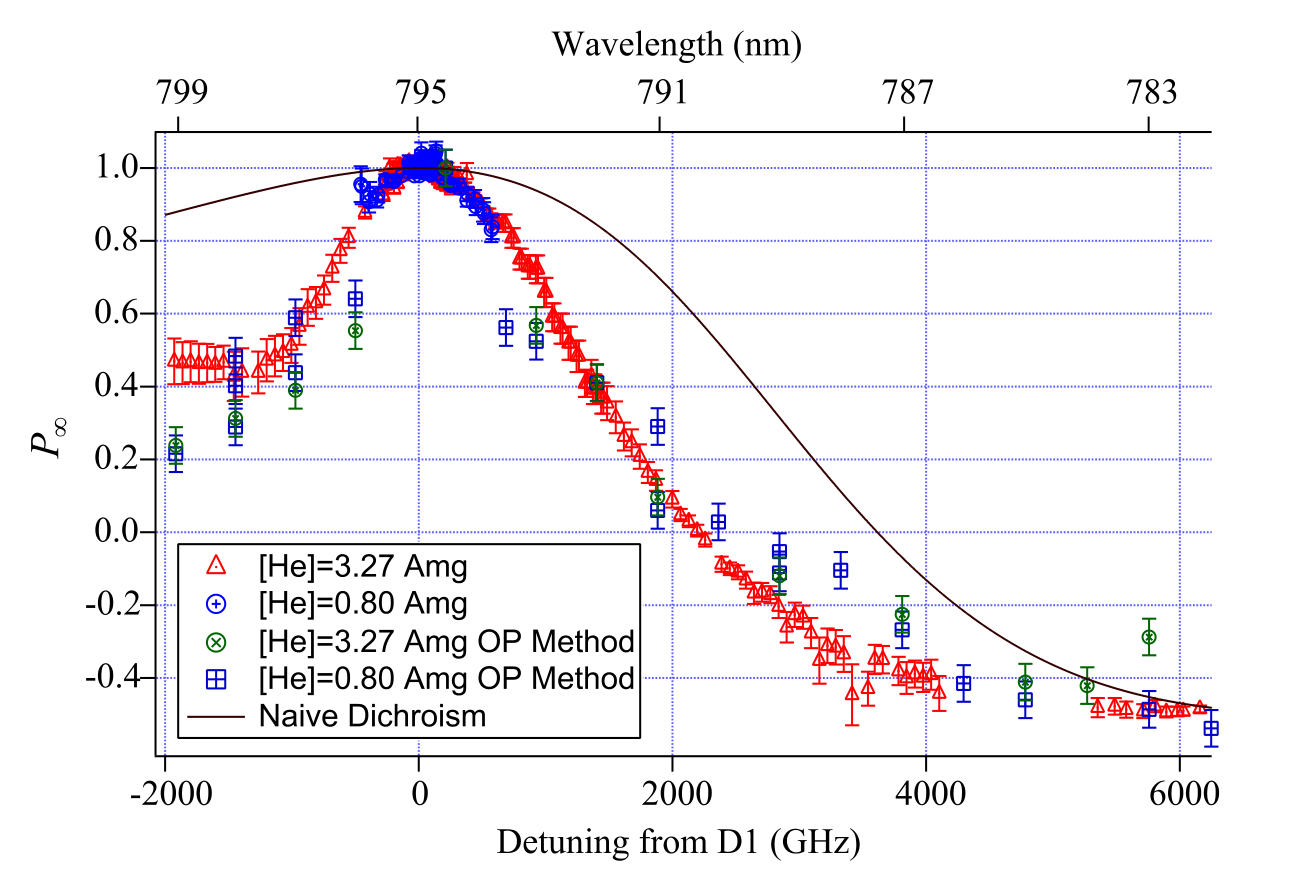
\includegraphics[width=\textwidth]{figures/chapter3-figs/dichroism.png}
    \caption[The maximum attainable alkali dichroism of Rb atoms in $^3$He.]{The maximum attainable alkali dichroism of Rb atoms in $^3$He. At the D1 resonance line of Rb, 795nm, the measured alkali polarization approaches 1. The solid line is the calculated dichroism without alkali-$^3$He collisions. Figure is taken from \cite{Gentile2017} with the original data in \cite{Lancor2010}.}
    \label{fig:dichroism}
\end{figure}
\clearpage}

\Cref{fig:dichroism} show measurement results of the dichroism\footnote{Dichroism means polarization dependent absorption.} of polarized Rb atoms in the presence of different densities of $^3$He \cite{Lancor2010}. The figure shows that while the alkali polarization peaks at the D1 resonance, a 1 nm detuning from the resonance drops the maximum alkali polarization to 0.9. This emphasizes the need for narrow-bandwidth lasers for yielding efficient optical pumping as well as higher maximum polarization.

The optical light scattering rate, $\mathcal{A}({\bf x})$, can be written as \cite{Gentile2017, Walker1997}:
\begin{equation}
\begin{split}
        \mathcal{A}({\bf x}) & = R({\bf x}) \left[ 1 - (P_{\infty}P_{A}) \right] \\
        & = \Gamma_A P_{\infty} P_{A}({\bf x}) - R({\bf x})(1-P_{\infty}^2)
\end{split}
\end{equation}
The first term compensates for collisions causing spin relaxation and the second term accounts for the light scattering from any off D1 line pumping \cite{Happer1987, Happer2010, Lancor2010}. In optical pumping, the light fluence rate or light flux density, $I({\bf x}) [cm^{-2}s^{-1}]$ at a location in the cell, {\bf x}, can be described as:
\label{eq:fluxdensity}
\begin{flalign}
    \frac{dI({\bf x})}{d{\bf x}} & = \mathcal{A}({\bf x})[A] \\ \nonumber
    & = [A]\Gamma_A P_{\infty} P_{A}({\bf x}) - [A]R({\bf x})(1-P_{\infty}^2) \\
    & = [A]\Gamma_A P_{\infty} P_{A}({\bf x}) - [A] \sigma_A I({\bf x})(1-P_{\infty}^2) \nonumber
    \label{eq:fluxdensity}
\end{flalign}
where [A] is the alkali concentration and the optical cross section, $\sigma_A$, for unpolarized alkali atoms is defined as the ratio of the optical pumping rate $R({\bf x})$ to the light flux density$I({\bf x})$ \cite{Appelt1998, Gentile2017}. If on D1 line pumping ($P_A \approx P_{\infty} = 1$), the first term in the equation leads to a linear attenuation in light flux density $I=I_0-[A]\Gamma_A P_{\infty}^2{\bf x}$ \cite{Bhaskar1979, Walker1997}. This means that the D1 light gets attenuated from the spin relaxation collisions despite the optical thickness of SEOP cells. If off D1 line pumping ($P_{\infty} < 1$), \cref{eq:fluxdensity} leads to an exponential attenuation of the light as $I=I_0 \exp \left ( - [A] \sigma (1-P_{\infty}^2){\bf x} \right )$ because the absorption length increases by a factor $\frac{1}{1-P_{\infty}^2}$ as compared to the absorption length under uniformly polarized alkali atoms \cite{Gentile2017}. 

Scattering of light also happens during off D1 line dichroism \cite{Babcock2003}. A light absorption efficiency defined as a the ratio of the production rate of polarized $^3$He to the light scattering \cite{Babcock2003}, can be used to characterize this:
\begin{equation}
    \eta_{\gamma} = \frac{[He]\frac{dP_{He}}{dt}}{[A]\mathcal{A}}
\end{equation}
where [He] is the concentration of He in the cell. Measured light absorption efficiency for optical pumping with a broad spectrum laser is shown in \cref{fig:lightefficiency}. This indicates that for optical pumping under off D1 line, the is light absorption becomes inefficient, due to light scattering \cite{Babcock2003}.

\afterpage{
\begin{figure}
    \centering
    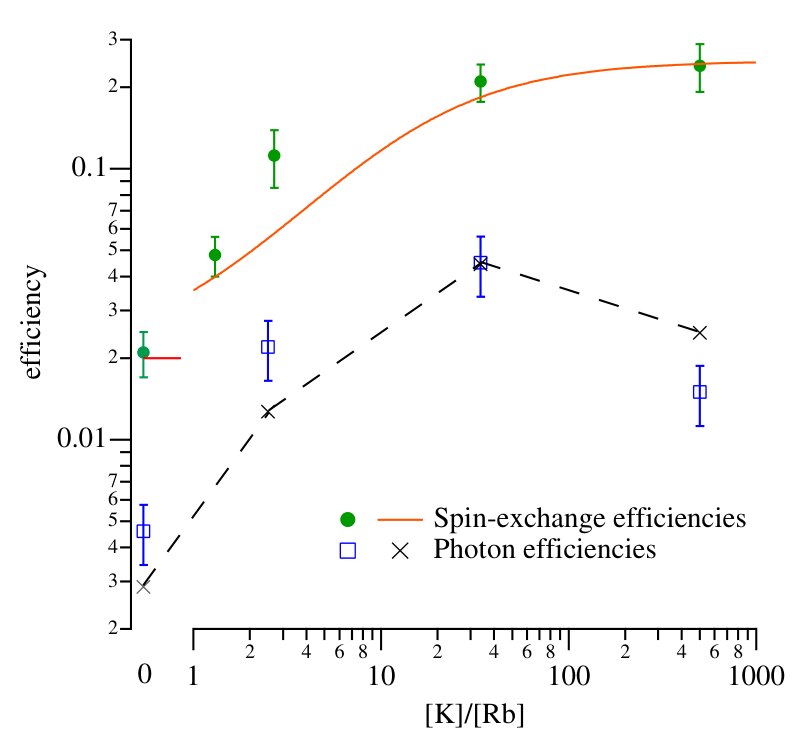
\includegraphics[width=\textwidth]{figures/chapter3-figs/SEeff_forD.png}
    \caption[Measured spin exchange and light absorption efficiencies as a function of alkali mixture concentration.]{Measured spin exchange and light absorption efficiencies as a function of alkali mixture concentration. The light absorption is  inefficient as compared to the maximum spin transfer efficiency due to the non-dichroism effects. Figure is taken from \cite{Gentile2017} with the original data and calculation from \cite{Babcock2003}.}
    \label{fig:lightefficiency}
\end{figure}
\clearpage}

In the early days, SEOP polarization of $^3$He used to struggle due to expensive, bulky, low power and broad spectral width laser technology \cite{Chupp1987, Wagshul1989, Coulter1990}. With the introduction of narrower laser diodes and compact Variable Bragg Gratings with integrated cooling systems in recent years, SEOP performance and attainable $^3$He polarization has increased \cite{Volodin2004, Chen2014}. These new lasers generally produce monochromatic light with a spectral width $<$ 0.2 nm (90 GHz), matching to the alkali D1 transition line, increasing the maximum attainable alkali polarization $P_{\infty}$. 

Other effects such as aberration of the incident laser light from uneven glass cells, changes in the laser beam divergence by glass and variation in the spatial modes of laser light can also prevent a uniform optical pumping rate along the volume of the cell \cite{Chann2003, Chen2014}. Although these factors can be somewhat mitigated by laser pumping the cell from both directions, a comprehensive study of the effect and mitigation of these factors on optical pumping has not been performed \cite{Chann2003, Chen2014}.


\subsection{Spin Exchange}

The exchange of spin angular momentum between the alkali and the $^3$He can be thought of as:
\begin{equation}
    A \uparrow + ^3He \downarrow \leftrightarrow A \downarrow + ^3He \uparrow
\end{equation}

The interaction potentials experienced during alkali-$^3$He collisions are
\begin{equation}
    V \propto V_0 + \Vec{S} \cdot \Vec{I}_{He} + \Vec{S} \cdot \Vec{N}
\label{eq:SEpot}
\end{equation}
where,
\begin{itemize}
    \item $V_0$ is the spin-independent interaction potential between the alkali-$^3$He \cite{Partridge2001, Tscherbul2011}.
    \item $\Vec{S} \cdot \Vec{I}_{He}$ is the hyperfine interaction between the alkali electron spin, $\Vec{S}$, and the $^3$He nuclear spin, $\Vec{I}_{He}$ \cite{Partridge2001, Tscherbul2011}.
    \item $\Vec{S} \cdot \Vec{N}$ is the alkali spin and alkali-$^3$He pair rotational angular momentum interaction \cite{Walker1997}. As discussed earlier, this is one of the known sources of spin relaxation in alkali and limits the spin exchange efficiency.
\end{itemize}

\afterpage{
\begin{figure}
    \centering
    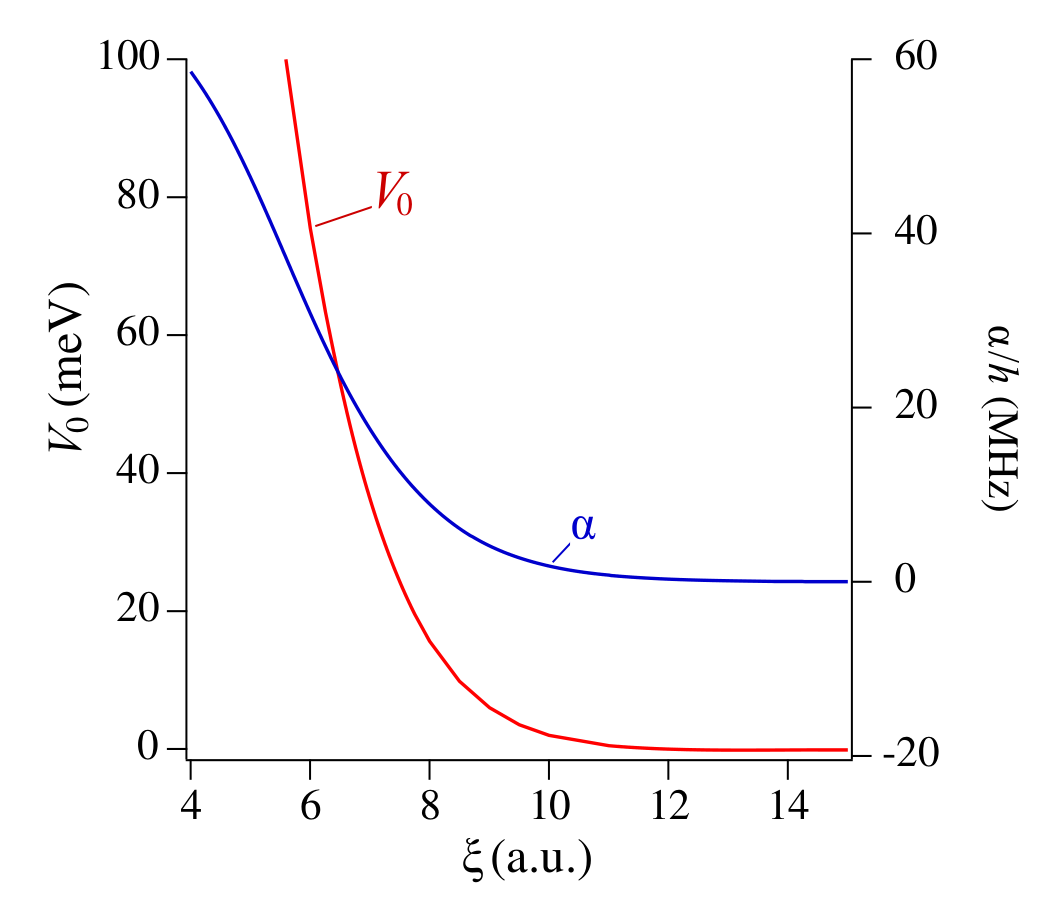
\includegraphics[width=\textwidth]{figures/chapter3-figs/SEpotentials.png}
    \caption[Calculated $V_0(x)$ and  $\Vec{S} \cdot \Vec{I_{He}}$ as a function of interatomic distance, $\xi$, for the K-$^3$He pair.]{Calculated $V_0(x)$ \cite{Partridge2001} and  $\Vec{S} \cdot \Vec{I_{He}}$ \cite{Tscherbul2011} for the K-$^3$He pair. Figure is taken from \cite{Gentile2017}.}
    \label{fig:spinexpot}
\end{figure}
\clearpage}

The interaction potentials, as shown in \cref{fig:spinexpot}, can be used to calculate the alkali-$^3$He spin-exchange rate, $k_{SE}$ \cite{Partridge2001, Tscherbul2011}. For K-$^3$He, the $k_{SE}$ comes out to be around $6 \times 10^{-20}$ cm$^3$s$^{-1}$ \cite{Gentile2017, Happer1972, Walker1997}. For typical alkali concentrations used in SEOP in the range of $10^{14}$ cm$^{-3}$ to $10^{15}$ cm$^{-3}$, the probability of spin exchange is very low and the spin-exchange time constant, $1/k_{SE}$, is around 10 to 50 hours \cite{Gentile2017}. This impresses the importance of building $^3$He cells with long lifetimes to achieve high $^3$He polarization.

The spin exchange and the relaxation/build up of polarized $^3$He, $P_{He}$, (mostly due to wall relaxation with rate, $\Gamma_{wall}$) can be modeled as \cite{Wu2021}:
\begin{equation}
    \frac{dP_{He}}{dt} = k_{SE} [A] (P_{A} -P_{He}) - \Gamma_{wall} P_{He}
\end{equation}
Since the $P_{He}$ varies on the scale of hours as compared to the alkali-metal electron polarization $P_{A}$, which varies with millisecond relaxation times, $P_{A}$ can be treated as constant. Thus, in a steady state solution, $P_{He}$ builds up as
\begin{equation}
    P_{He, \infty} = P_{A} \frac{k_{SE} [A]}{k_{SE} [A] + \Gamma_{wall}}
\end{equation}
at a time constant of
\begin{equation}
    \frac{1}{\tau} = k_{SE} [A] + \Gamma_{wall}
    \label{eq:SEtime}
\end{equation}
This linear relation implies that one can measure $k_{SE}$, and in effect the build up of $P_{He, \infty}$, by measuring the time constant as a function of the alkali concentration, [A] \cite{Gentile2017}. However, as will be described later, $\Gamma_{wall}$, has been found to vary non-linearly as a function of temperature of the $^3$He cell and only wall loss relaxation independent methods have to be used to measure $k_{SE}$ \cite{Gentile2017}. The no SEOP re-polarization method \cite{Ben-AmarBaranga1998, Chann2002a, Borel2003}, the rate balance method \cite{Chann2002a}, the $^4$He exchange rate method \cite{Walker2010}, and the absolute alkali polarimetry method \cite{Singh2015} have been used to measure the spin-exchange rate, $k_{SE}$ for the different alkali. The results from these measurements are shown in \cref{tab:spinexrate}

\afterpage{
\begin{table}
\centering
\caption[Measurements of spin-exchange rate coefficient using wall-independent methods all normalized to  the EPR frequency shift factors]{Measurements of spin-exchange rate coefficient $k_{SE}$, using wall-independent methods, all normalized to the EPR frequency shift factors $\kappa_0$ and $\frac{d\kappa_0}{dT}$. Data taken from \cite{Ben-AmarBaranga1998, Chann2002a, Borel2003, Walker2010, Singh2015}.}
\label{tab:spinexrate}
\begin{tabular}{@{}lccc@{}}
\toprule
 & Na & K & Rb \\ \midrule
$k_{SE} $ [$10^{-20}$ cm$^{3}$s$^{-1}$] & 6.1 & 6.1-7.5 & 6.7-6.8 \\
$\kappa_0$ & 4.7 & 6.0 & 6.1 \\
$\frac{d\kappa_0}{dT}$ [K$^{-1}]$ & 0.009 & 0.008 & 0.009 \\ \bottomrule
\end{tabular}
\end{table}
\clearpage}

Even though the spin exchange from alkali to $^3$He is limited with a slow time constant, the efficiency of the optically pumping to polarize the alkali is high. If no light scattering from polarized alkali atoms is assumed, the loss of angular momentum by polarized alkali-metal atoms happens at a rate [A] V $\Gamma_A P_A$. At the same time, the addition of angular momentum to $^3$He happens as,  V[He]$\frac{dP_{He}}{dt}$, the spin exchange collision efficiency can be written as \cite{Gentile2017, Ben-AmarBaranga1998}:
\begin{equation}
    \eta = \frac{V [He] \frac{dP_{He}}{dt}}{[A] V \Gamma_A P_A} = \frac{k_{SE} [He]}{\Gamma_A} \left (  1- \frac{P_{He}}{P_{He, \infty}}             \right )
\end{equation}

This spin exchange collision efficiency is maximum during the early stages of SEOP at low $^3$He polarization, but then decreases as higher $^3$He polarization and alkali polarization approach equilibrium. This efficiency varies from alkali to alkali \cite{Ben-AmarBaranga1998}.

Although $\Gamma_A$ contributes to the alkali spin-relaxation rate, the minimum possible alkali spin-relaxation rate is $\Gamma_A = (k_{SE} + k_{SR}) $[He] , where $k_{SR}$ is the relaxation due to the the alkali spin and alkali-$^3$He pair rotational angular momentum interaction as discussed previously \cite{Ben-AmarBaranga1998, Borel2003, Singh2010}. This relaxation limits the spin exchange to:
\begin{equation}
    \eta = \frac{k_{SE}}{k_{SE} + k_{SR}}
\end{equation}
Measurements and expected values of the spin-exchange efficiency for the alkali elements, Na, K, Rb and Cs are shown in \cref{fig:SEeff}.

\afterpage{
\begin{figure}
    \centering
    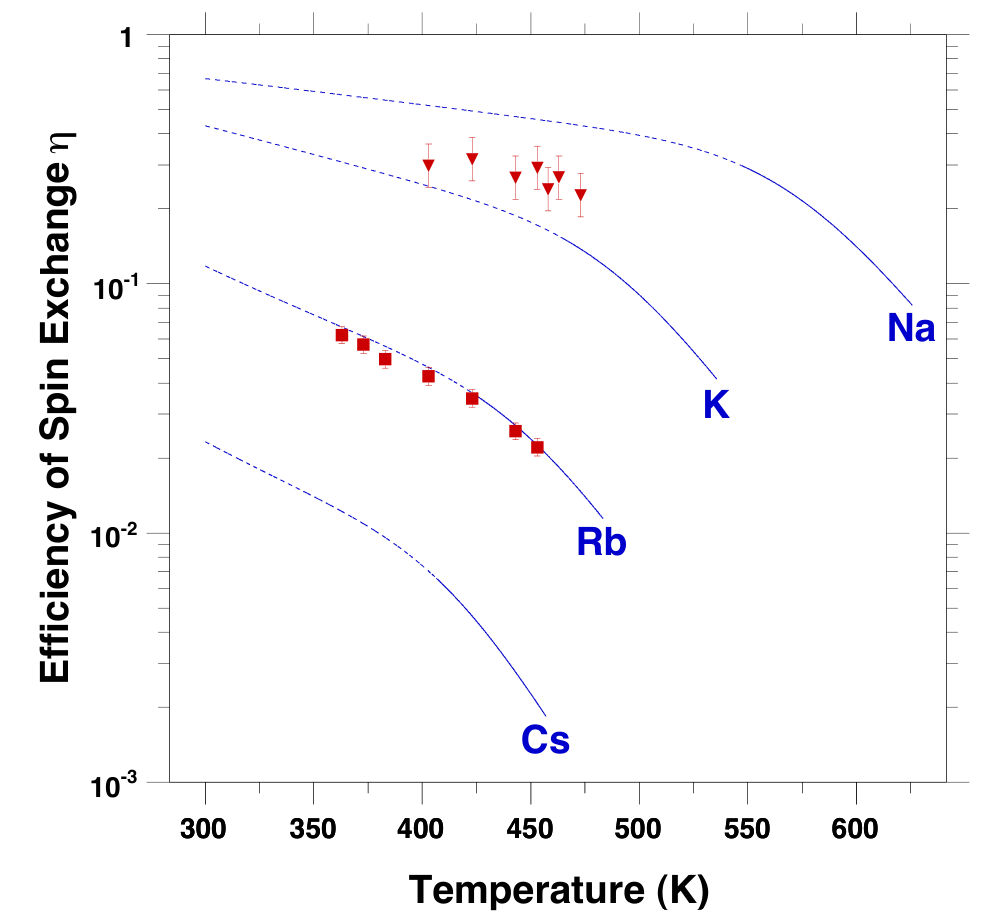
\includegraphics[width=\textwidth]{figures/chapter3-figs/SEeff.png}
    \caption[Spin Exchange Efficiencies for Na, K, Rb, \& Cs]{Spin Exchange Efficiencies for Na, K, Rb, \& Cs taken from \cite{Singh2010}. The blue lines are calculated from \cite{Singh2010} and the red data points are from \cite{Ben-AmarBaranga1998}. The SEOP described in the thesis performed at $^3$He cell temperature of 200 \degree C so the efficiency curves shown in this plot have to be extrapolated at those temperatures. Nonetheless, the efficiency trends shown in this figure looks to match the efficiency at 200 \degree C.}
    \label{fig:SEeff}
\end{figure}
\clearpage}

\subsection{SEOP with Hybrid Alkali}

\Cref{fig:SEeff} shows that of all the alkali elements, Na and K have the largest spin exchange efficiency as compared to Rb and Cs. Therefore, it is sensible to pursue SEOP using Na or K alkali atoms.\footnote{In terms of neutron scattering and absorption, Na, K, Rb can be used due to small neutron scattering and absorption cross sections. For Cs, the scattering cross section is a little large.} However, It is not yet possible to perform SEOP using Na because of the technological unavailability of 590 nm lasers at the D1 transitions of Na \cite{Borel2003}. This leaves us with K and Rb. Direct pumping of pure K based cells is also difficult due to potential unwanted optical pumping of the K D2 line in the fine-structure \cite{Chen2007}. Although at the level of 0.2 nm spectral width, 770 nm K D1 transition lasers have not yet reached $>$ 100 W power levels, \cite{Chen2007} found increased spin exchange efficiency using hybrid (K and Rb) alkali cells and this has become the standard approach for polarizing $^3$He using SEOP for neutron spin filters \cite{Chen2007, Chen2011}.  
In hybrid SEOP, a Rb/K mixture cells are used with higher concentration of K as compared to Rb \cite{Lancor2010, Lancor2011}. The Rb is optically pumped based on the Rb D1 line. Alkali-alkali spin-exchange leads the K atoms to become polarized as well. Since K has a smaller spin relaxation rate than Rb, the K-$^3$He spin exchange of angular momentum is more efficient as compared to Rb \cite{Lancor2010, Lancor2011}. Taking into account the total hybrid alkali spin-relaxation rate $\Gamma_{Rb}$ + $ \mathcal{D}$  $ \Gamma_K$, where $ \mathcal{D} $ = [K]/[Rb], the hybrid alkali spin-exchange efficiency becomes:
\begin{equation}
    \eta^{hybrid} = \frac{ (k_{SE}^{Rb} + \mathcal{D} k_{SE}^{K} ) [He]}{\Gamma_{Rb} + \mathcal{D}\Gamma_K}
\end{equation}
which for large $\mathcal{D}$, approaches $\eta_{SE}^{K}$ \cite{Lancor2010, Lancor2011}. This can be seen in the measurements of the spin-exchange efficiency for different concentrations of alkali mixture shown in \cref{fig:hybrideff}.

\afterpage{
\begin{figure}
    \centering
    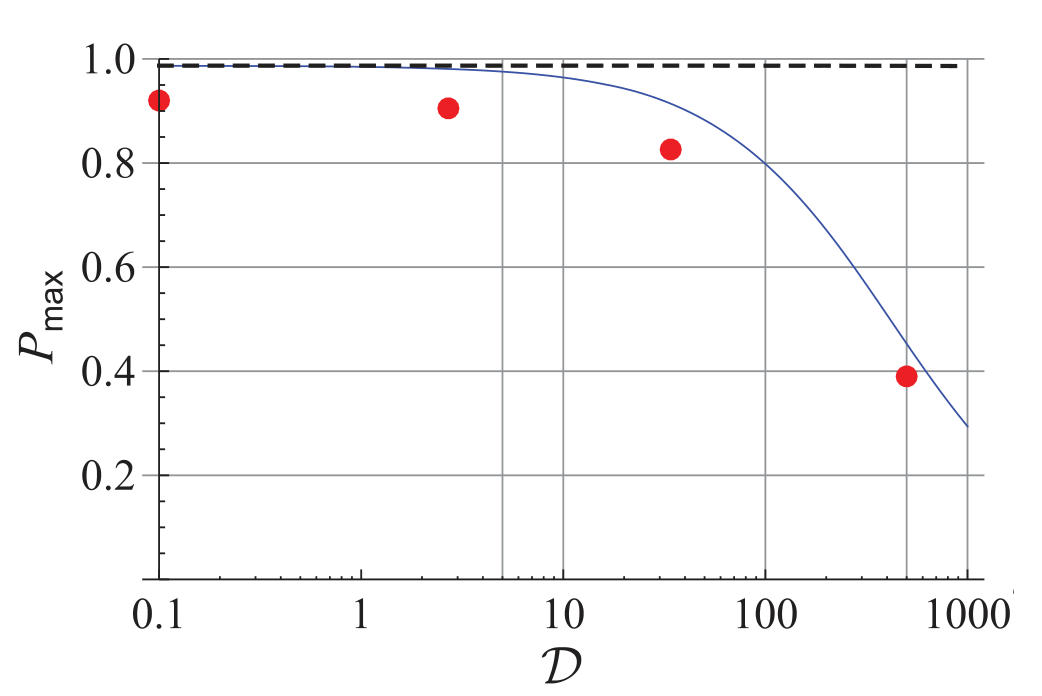
\includegraphics[width=\textwidth]{figures/chapter3-figs/Pmax_vs_D.png}
    \caption[Alkali polarization as a function of alkali ratio.]{Alkali polarization as a function of alkali mixture. Figure is taken from \cite{Gentile2017} with the original data in \cite{Lancor2010, Lancor2011}.}
    \label{fig:hybrideff}
\end{figure}
\clearpage}

The reduction in loss from collisions in hybrid SEOP allows for an increased alkali density and thus, an increased polarization rate and furthermore, a large volume of $^3$He to be polarized. $\mathcal{D}$ ratio between 2 and 7 is found to yield the best spin exchange efficiency \cite{Chen2007, Chen2011, Chen2014}. For neutron based $^3$He cells, $\mathcal{D}$ usually determined with relative peak intensities in white light absorption spectroscopy as well as monitoring optical pumping rate as a function of temperature \cite{Chen2007, Chen2011, Chen2014}.

\subsection{$^{3}$He Relaxation Mechanisms}

This section describes the mechanisms responsible for `relaxing', i.e. depolarizing the polarized $^3$He. The primary mechanisms are the dipole-dipole relaxation, wall effects and field gradients.

\cite{Newbury1993} found that $T_1$ longitudinal polarization relaxation time, characterizes relaxation of $^3$He polarized along the direction of holding magnetic field is limited by the dipole-dipole interactions within $^3$He to $\frac{1}{T_1} = \frac{P}{807} $ hours$^{-1}$, where P is pressure of the cell in bars. This relaxation, which occurs as $\exp(-t/T_1)$, has been verified for $^3$He cells with pressures of 2 to 12 bars \cite{Smith1998}. For neutron spin filters made of GE180 glass, with pressures of $\sim$1bar and polarized via Rb or K-Rb SEOP, $T_1$ of several hundred hours has been observed \cite{Rich2002, Parnell2009, Chen2011}, and most likely attributed to formation of thin films of alkali coating the inner walls of the glass; suppressing wall relaxation \cite{Wu2021}.

A major limiting factor for a high achievable $T_1$ in a SEOP cell is the relaxation of polarized $^3$He with the glass cell walls. Yet, this effect is not fully understood despite being recognized since the very first SEOP $^3$He polarization experiment, where aluminosilicate glass yielded long relaxation times as compared to borosilicate glass \cite{Fitzsimmons1969}. Further studies have shown that $^3$He permeates the borosilicate glass whereas it adsorbs on the aluminosilicate glass \cite{Jacob2003, Gentile2017}. For aluminosilicate glass cells, longer $T_1$ time has been observed for cells kept at higher temperatures due to reduced adsorption on top of already negligible permeation \cite{Jacob2003}. This fact has led aluminosilicate glass based cells to become the standard for SEOP \footnote{Aluminosilicate glass is also resistant to alkali corrosion.}. For neutron beam based applications of $^3$He glass cells, this is incredibly useful because this avoids any attenuation of the neutron beam from possible boron content in the glass. It has also been found that tempered cells made from glass blowing, have been found to decrease $^3$He relaxation \cite{Rich2002, Parnell2009, Chen2011}.

Strong holding magnetic fields and physical orientation of the cell relative to the holding magnetic fields have also been found to have an effect on $^3$He relaxation. \cite{Chen2011} observed an order of magnitude decrease in $T_1$ with a holding field of 400 G. Interestingly, a ``hysteresis" was observed, where once 10 G to 30 G holding fields were applied, the high $T_1$ time was recovered. They also observed that $T_1$ can change, preferring to increase for a certain cell orientation i.e. $^3$He cells prefers to polarize only in certain physical orientations. 

The main culprit responsible for relaxation of polarized $^3$He in SEOP cells is presence of magnetic field gradients transverse to the holding field $B_0$, which causes the $^3$He polarization spins to precess non-adiabatically away from $B_0$ \cite{Gamblin1965, Schearer1965, Cates1988a, Cates1988b, McGregor1990, Bohler1994}. At room temperature and pressure, P in bars, a useful relation for the relaxation rate caused by a field gradient, in units of hours$^{-1}$, is given by \cite{McIver2009}:
\begin{equation}
    \frac{1}{T_1} = \frac{6700}{P} \left ( \frac{\left \lvert \Vec{\nabla} B_{\perp} \right \rvert ^2}{B_0^2} \right )
\label{eq:gradT1}
\end{equation}
where $ \frac{ \left \lvert \Vec{\nabla} B_{\perp} \right \rvert}{B_0}$ is the transverse gradient in the longitudinal magnetic field, in units of cm$^{-1}$, assuming longitudinal polarization is along the z-axis \cite{Cates1988b}. For a 1 bar cell in a uniform gradient of
\begin{equation}
     \frac{ \left \lvert \Vec{\nabla} B_{\perp} \right \rvert}{B_0} \approx 3 \times 10^{-4}  ~\text{cm$^{-1}$}
\label{eq:gradstandard}
\end{equation}
the $^3$He polarization relaxation time, from the \cref{eq:gradT1}, comes out to be about 800 hours \footnote{This relation is only valid for when the $ \omega_{Larmor}^{He} \ll \frac{1}{\tau_{collisions}}$.} \cite{Chen2020}. This relaxation time is usually adequate for SEOP cells used in neutron based experiments and so the gradients listed in \cref{eq:gradstandard} are usually the standards for developing magnetostatic cavities for providing the uniform holding magnetic fields for the polarized $^3$He cell. In conjunction with the need for low field gradients, space constraints, stray fields, and neutron spin transport magnetic field matching have also motivated the development of novel magnetostatic cavities for polarized $^3$He gas. Magnetically shielded solenoids and coils are typically employed to achieve this. Magnetic shielding and uniformity is provided via high magnetic permeability materials like mu-metal. $\cos \theta$ coils, double $\cos \theta$ coils and Merrit coils \cite{Merritt1983, Babcock2019, Chen2020}, enveloped by mu-metal shielding, have been used recently to achieve gradients between $6 \times 10^{-4} $ cm$^{-1}$ and $2 \times 10^{-4} $ cm$^{-1}$, corresponding to $^3$He polarization relaxation times between nearly 600 hours and 4000 hours, respectively \cite{Chen2014}.

\subsection{Limitations to $^{3}$He Polarization}

The previous sections describe how polarizing alkali via optical pumping, making glass cells with long wall-relaxation times, making making holding magnetic fields with low gradients, and utilizing hybrid alkali optical pumping for efficient spin exchange, should lead to very high $^3$He polarizations. In this section, the known systematic effects, which limit the maximum attainable $^3$He polarization are described.  

There is an anisotropic spin exchange alkali-$^3$He interaction, caused by the long-range $^3$He nuclear magnetization,
\begin{equation}
    V \propto  \Vec{S} \cdot \Vec{I_{He}}
\end{equation}
which polarizes the $^3$He nuclei as $ P_{He} \propto - P_A $, and therefore, limits the maximum attainable $^3$He polarization as
\begin{equation}
    P_{He, \infty} \le 1 - \frac{3 k_{S\cdot I}}{ 2 k_{hf}}
\end{equation}
Here $k_{hf}$ is the rate coefficient due to the hyperfine interaction from \cref{eq:SEpot} and $k_{S\cdot I}$ is the rate coefficient due to the anisotropic interaction \cite{Walter1998}. A calculation of this interaction limits the maximum attainable $^3$He polarization to $P_{He, \infty} \approx 0.95$ for SEOP \cite{Walter1998, Tscherbul2011}. So far, there have been no definitive measurements of anisotropic spin exchange contribution towards $^3$He polarization.

\afterpage{
\begin{figure}
    \centering
    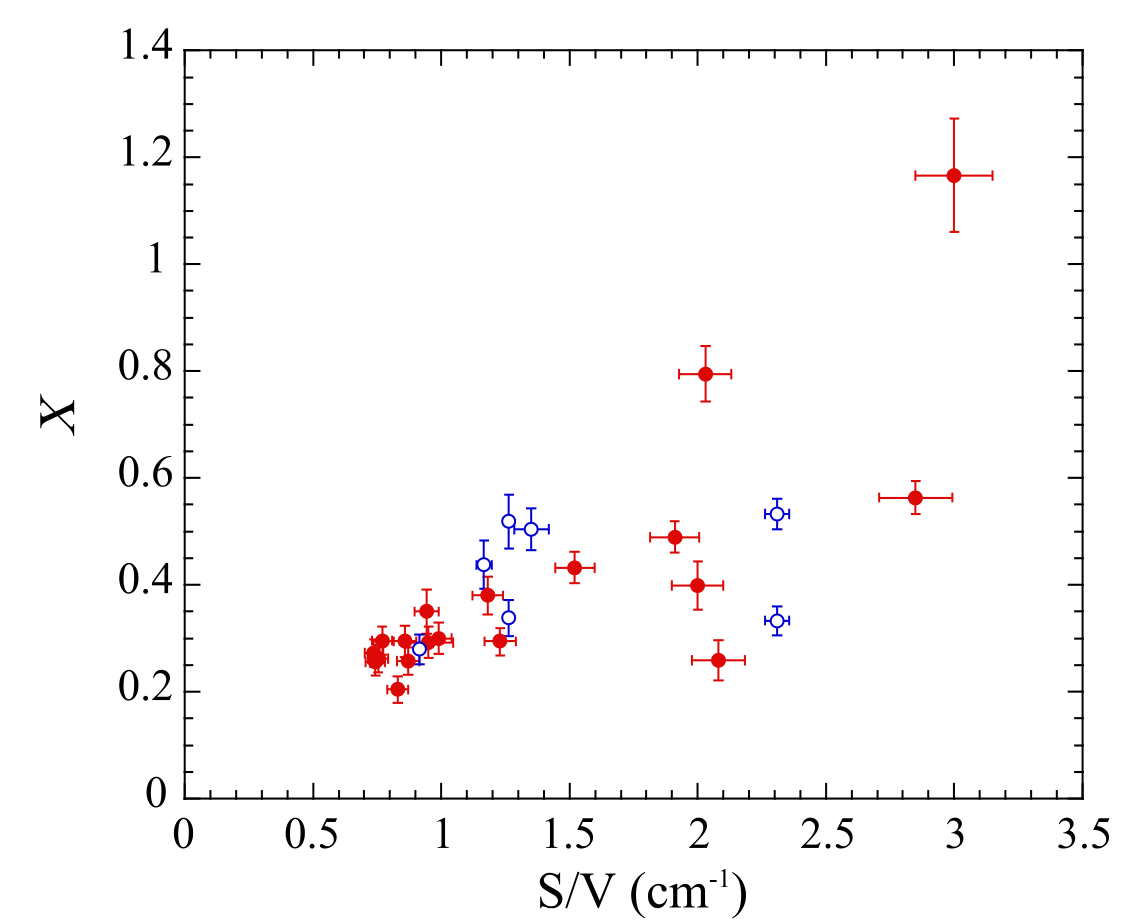
\includegraphics[width=\textwidth]{figures/chapter3-figs/Xfactor.png}
    \caption[Characterization of the X factor for spherical glass cells (red) and cylindrical glass cells (blue) as a function of the cell surface area to volume ratio.]{Characterization of the X factor for spherical glass cells (solid, red) and cylindrical glass cells (open, blue) as a function of the cell surface area to volume ratio. Figure is taken from \cite{Gentile2017} and the measurements were performed at NIST \cite{Babcock2006}.}
    \label{fig:Xfactor}
\end{figure}
\clearpage}

The second systematic effect, which limits the $^3$He polarization, is called the ``X-factor". Phenomenological studies of the spin exchange characteristic time, \cref{eq:SEtime}, use the relation:
\begin{equation}
    \frac{1}{\tau} = k_{SE} (1 + X) [A] + \Gamma_{wall}
\end{equation}
where $\Gamma_{wall}$ is the room temperature relaxation rate \cite{Chann2002a, Chann2003, Babcock2006, Chen2007, Walker2011, Chen2014, Singh2015}. This relation arises from the fact that the polarized $^3$He wall-relaxation rate has an excess term which increases exponentially as a function of temperature \cite{ Chann2003, Babcock2006, Walker2011, Chen2014, Singh2015}. This term limits the $^3$He polarization to
\begin{equation}
    P_{He, \infty} \le \frac{1}{1+X}
\end{equation}
assuming full alkali polarization and neglecting $\Gamma_{wall}$. This ``X factor", has been verified experimentally for both pure and hybrid cells with large variations across many different cells \cite{Chann2002a, Chann2003, Babcock2006, Chen2007, Walker2011, Chen2014, Singh2015}. This variation is what hints towards a possible temperature dependence, however the true cause of this effect is still unknown \cite{Chann2002a, Chann2003, Babcock2006, Chen2007, Walker2011, Chen2014, Singh2015}. Direct measurements of the ``X factor" have been performed by measuring the $^3$He relaxation in heated cells by parameterizing the ``X factor" as a function of the ratio of the surface area of cell to cell volume \cite{Babcock2006}. They are shown in \cref{fig:Xfactor}. These measurements were consistent with the highest possible $^3$He polarization observed so far of 75\% to 80\% \cite{Parnell2009, Ye2010, Singh2015}.

The third effect which can limit the $^3$He polarization is the fact that the $^3$He polarization is restricted by the spatial distribution of polarized alkali, especially when spin relaxation rates are negligibly small compared to spin exchange rates \cite{Gentile2017, Anderson2020}. Due to the high pressures used in SEOP, the diffusion of polarized alkali in the cell volume can be small, which means all regions of the cell must be illuminated by the laser for a useful SEOP. It is also important to characterize the spectrum of the residual transmitted light from the cell, verifying the depletion of D1 line laser light \cite{Lancor2011}.

\section{In situ Polarized $^{3}$He Cell}

As mentioned earlier in this chapter, polarized $^3$He cells can be thought of as a neutron spin filter (NSF) with the purpose of either producing beams of spin-polarized low-energy neutrons, or analyzing the spin-polarized state of a neutron beam. \cite{Ioffe2011}. The NSF’s ability to do this with near very good spin contrast comes from the spin dependence of the $^3$He neutron absorption cross section \cite{Coulter1990, Passell1966}. Other devices such as supermirrors \cite{Mezei1976} and Heusler crystals can also be used to provide near perfect neutron polarization and spin analysis \cite{Williams1988}. However, the operation of these devices is highly dependent upon the angular divergence and wavelength of the neutron beam. In contrast, NSFs are advantageous because they allow for the spin polarization to be decoupled from these beam effects. 

%Recently, there has been an increase in deploying in situ SEOP based NSF systems at the neutron beamline. These systems have a built-in oven for heating, an embedded laser system along with the optics, internal NMR system for polarized $^3$He control, and a magnetostatic cavity to provide the holding magnetic field.

$^3$He cells or NSFs are usually polarized by SEOP or MEOP in dedicated optical pumping stations in external laboratories \cite{Jiang2023}. After the $^3$He cell is polarization, the cell is relocated to the neutron experiment in a portable magnetostatic cavity \footnote{Neutron beam polarimetry for former experiments at the SNS beamline 13 was performed using $^3$He cells polarized off site.}. This ex situ deployment of polarized $^3$He has a problem: The $^3$He polarization undergoes exponential decay as soon as SEOP is turned off \cite{Jiang2023}. This decaying $^3$He polarization will inhibit the $^3$He cell's efficacy as a NSF, making it useful only for a limited time \cite{Jiang2017, Jiang2023}. Afterwards, the cell must return to the external optical pumping station for repolarization \cite{Jiang2017, Jiang2023}. Since the neutron polarization and transmission are changing with the decaying $^3$He polarization, the data analysis also becomes complicated. An in situ SEOP $^3$He polarization system would keep the saturated $^3$He cell polarization stable since the polarized $^3$He would undergo SEOP continuously, and not decay. Recently, SEOP-based compact in situ polarized $^3$He neutron spin filters have been developed to be utilized for neutron beam experiments at the Oak Ridge National Laboratory (ORNL) \cite{Tong2012, Jiang2014, Jiang2017, Jiang2023}. These systems can be deployed directly at the neutron beamline. In this section, the setup, assembly and performance testing of an in situ $^3$He polarizer for the beamline 13A is described.

The design model for the in situ $^3$He SEOP polarizer is shown in \cref{fig:insitu_side}. It is designed so that the neutron beam will traverse through the sapphire beam portals without any interference with the SEOP components as indicated in the \cref{fig:insitu_topdown}. \Cref{fig:insitupic} shows the in situ system undergoing assembly and performance at the SNS laser laboratory. The main components of the in situ system are (i) the laser head and interlocked laser enclosure, (ii) the cell heating system (iii) the light optics and (iv) the magnetic field coil and shielding.

\afterpage{
\begin{figure}
    \centering
    \begin{subfigure}[b]{0.8\textwidth}
        \centering
         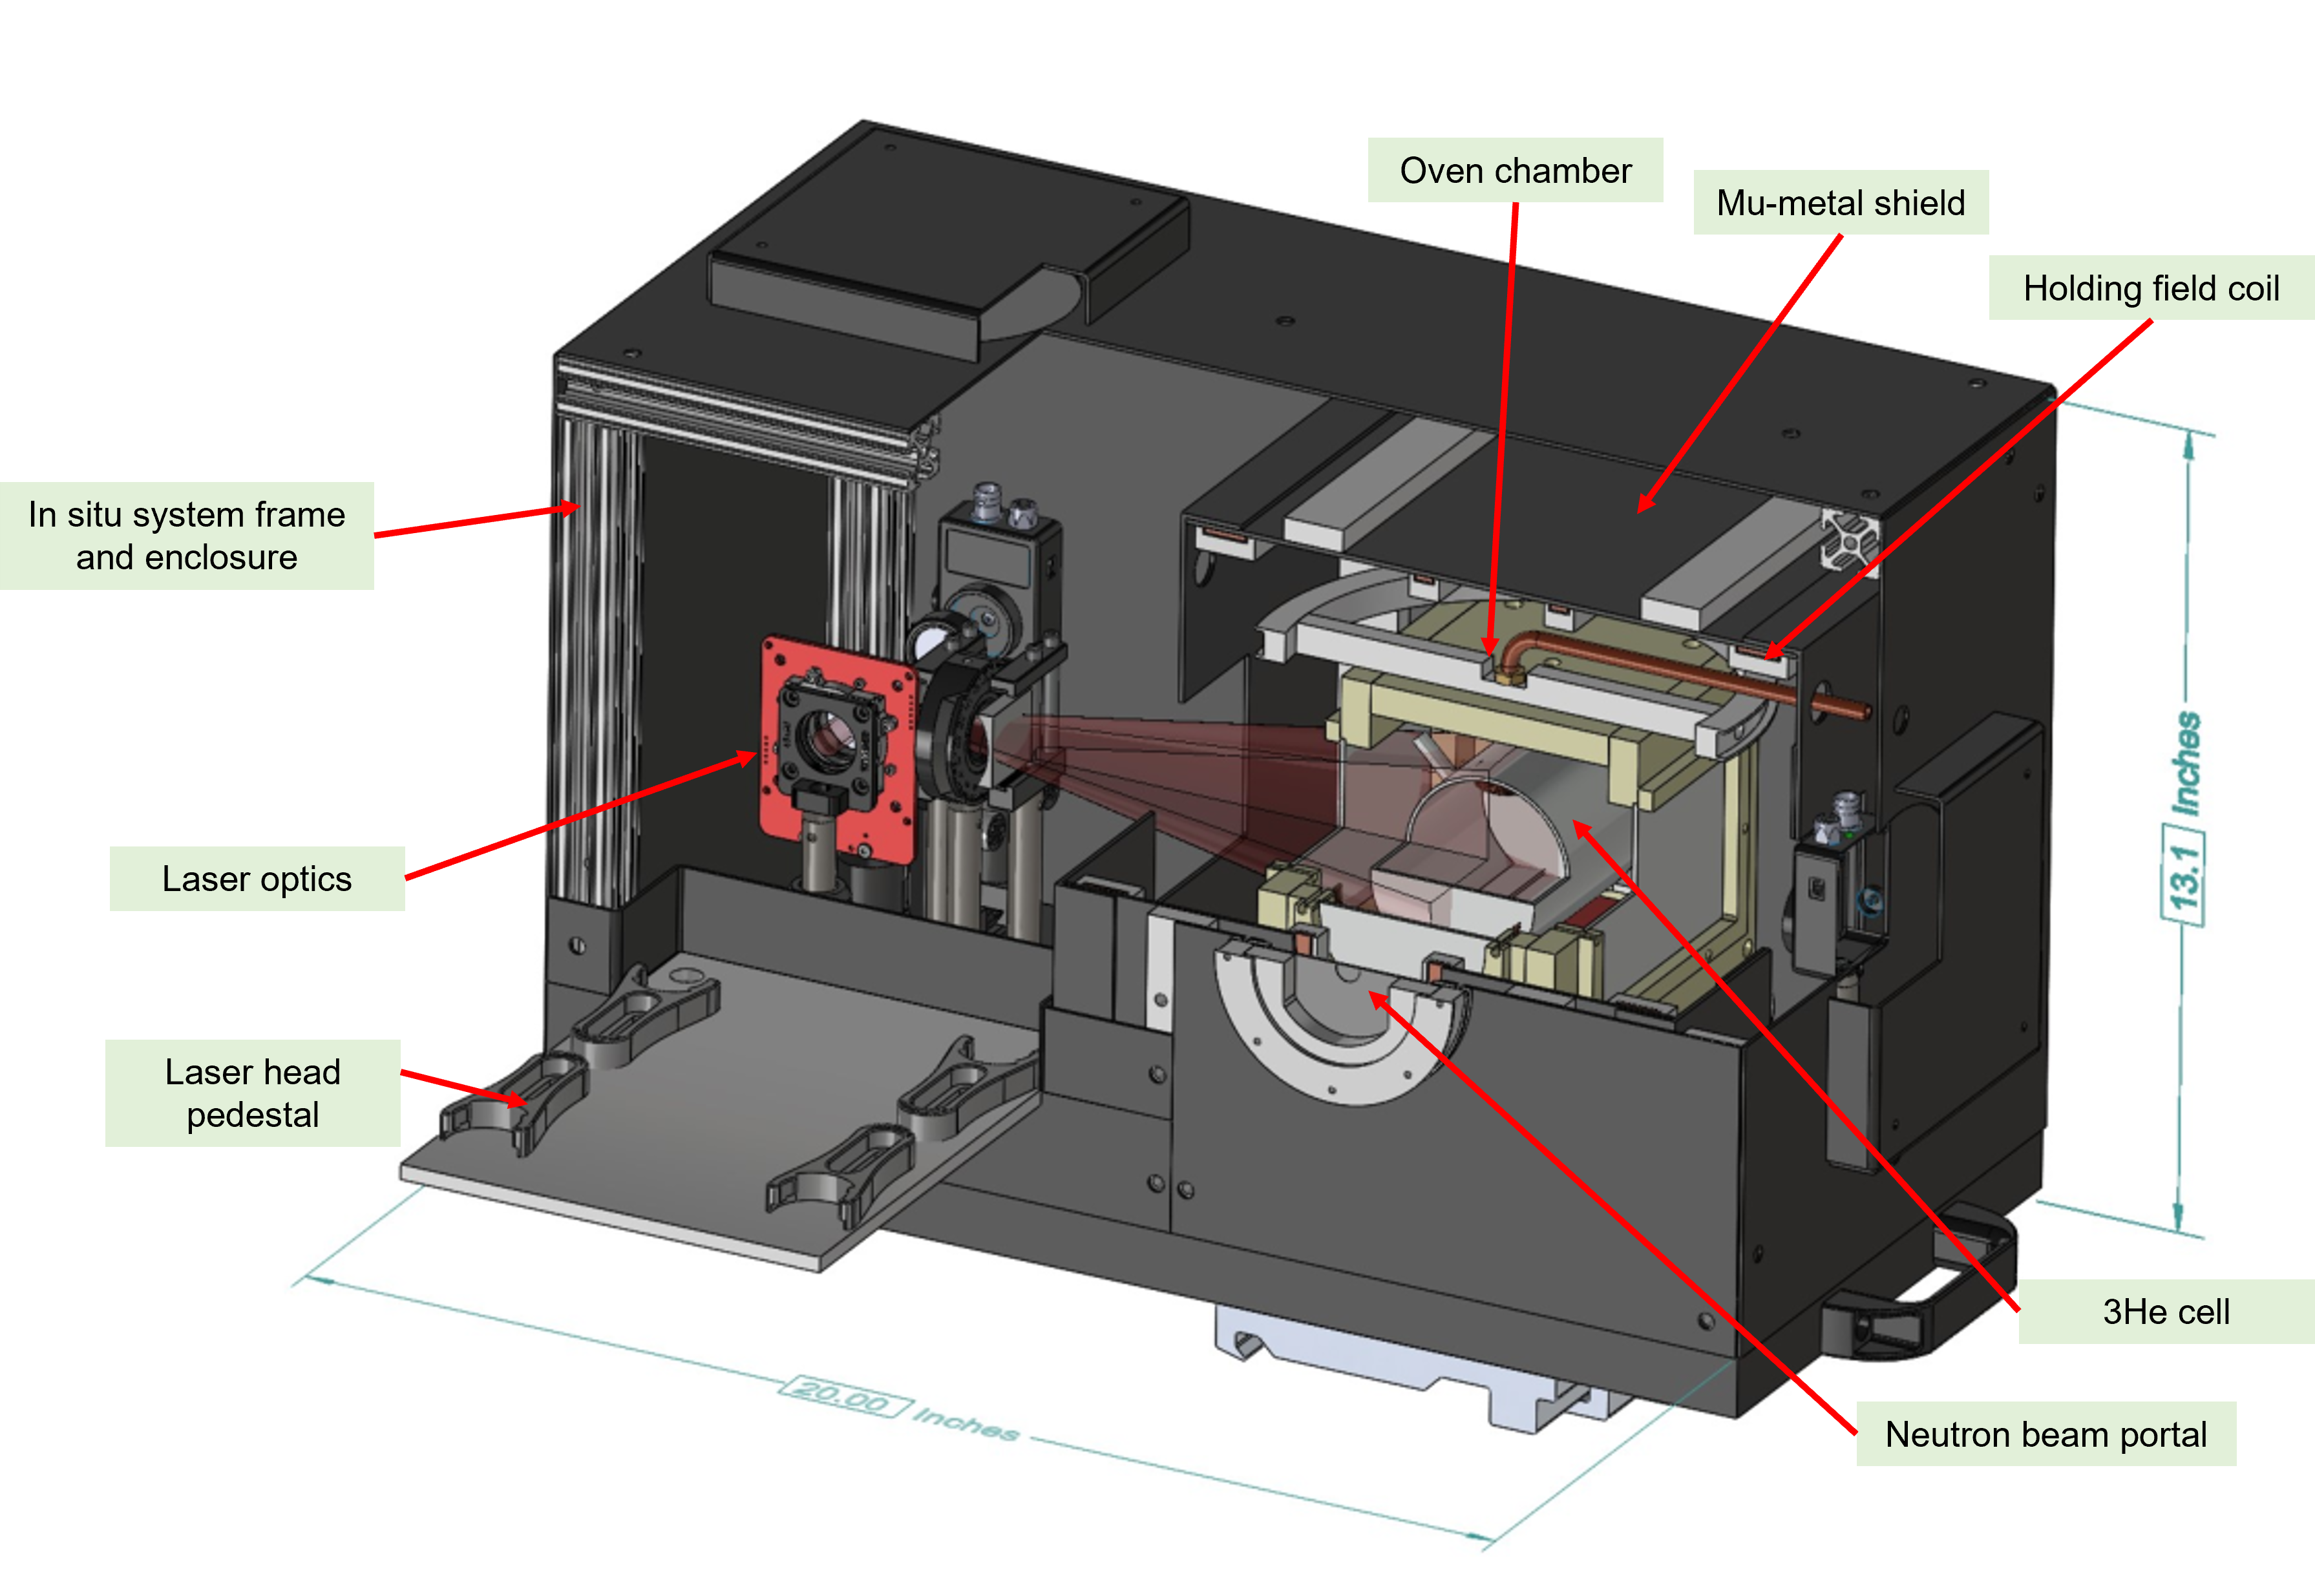
\includegraphics[width=\textwidth]{figures/chapter3-figs/insitumodel.png}
         \caption{Side view.}
         \label{fig:insitu_side}
     \end{subfigure}
     \hfill
     \begin{subfigure}[b]{0.8\textwidth}
        \centering
         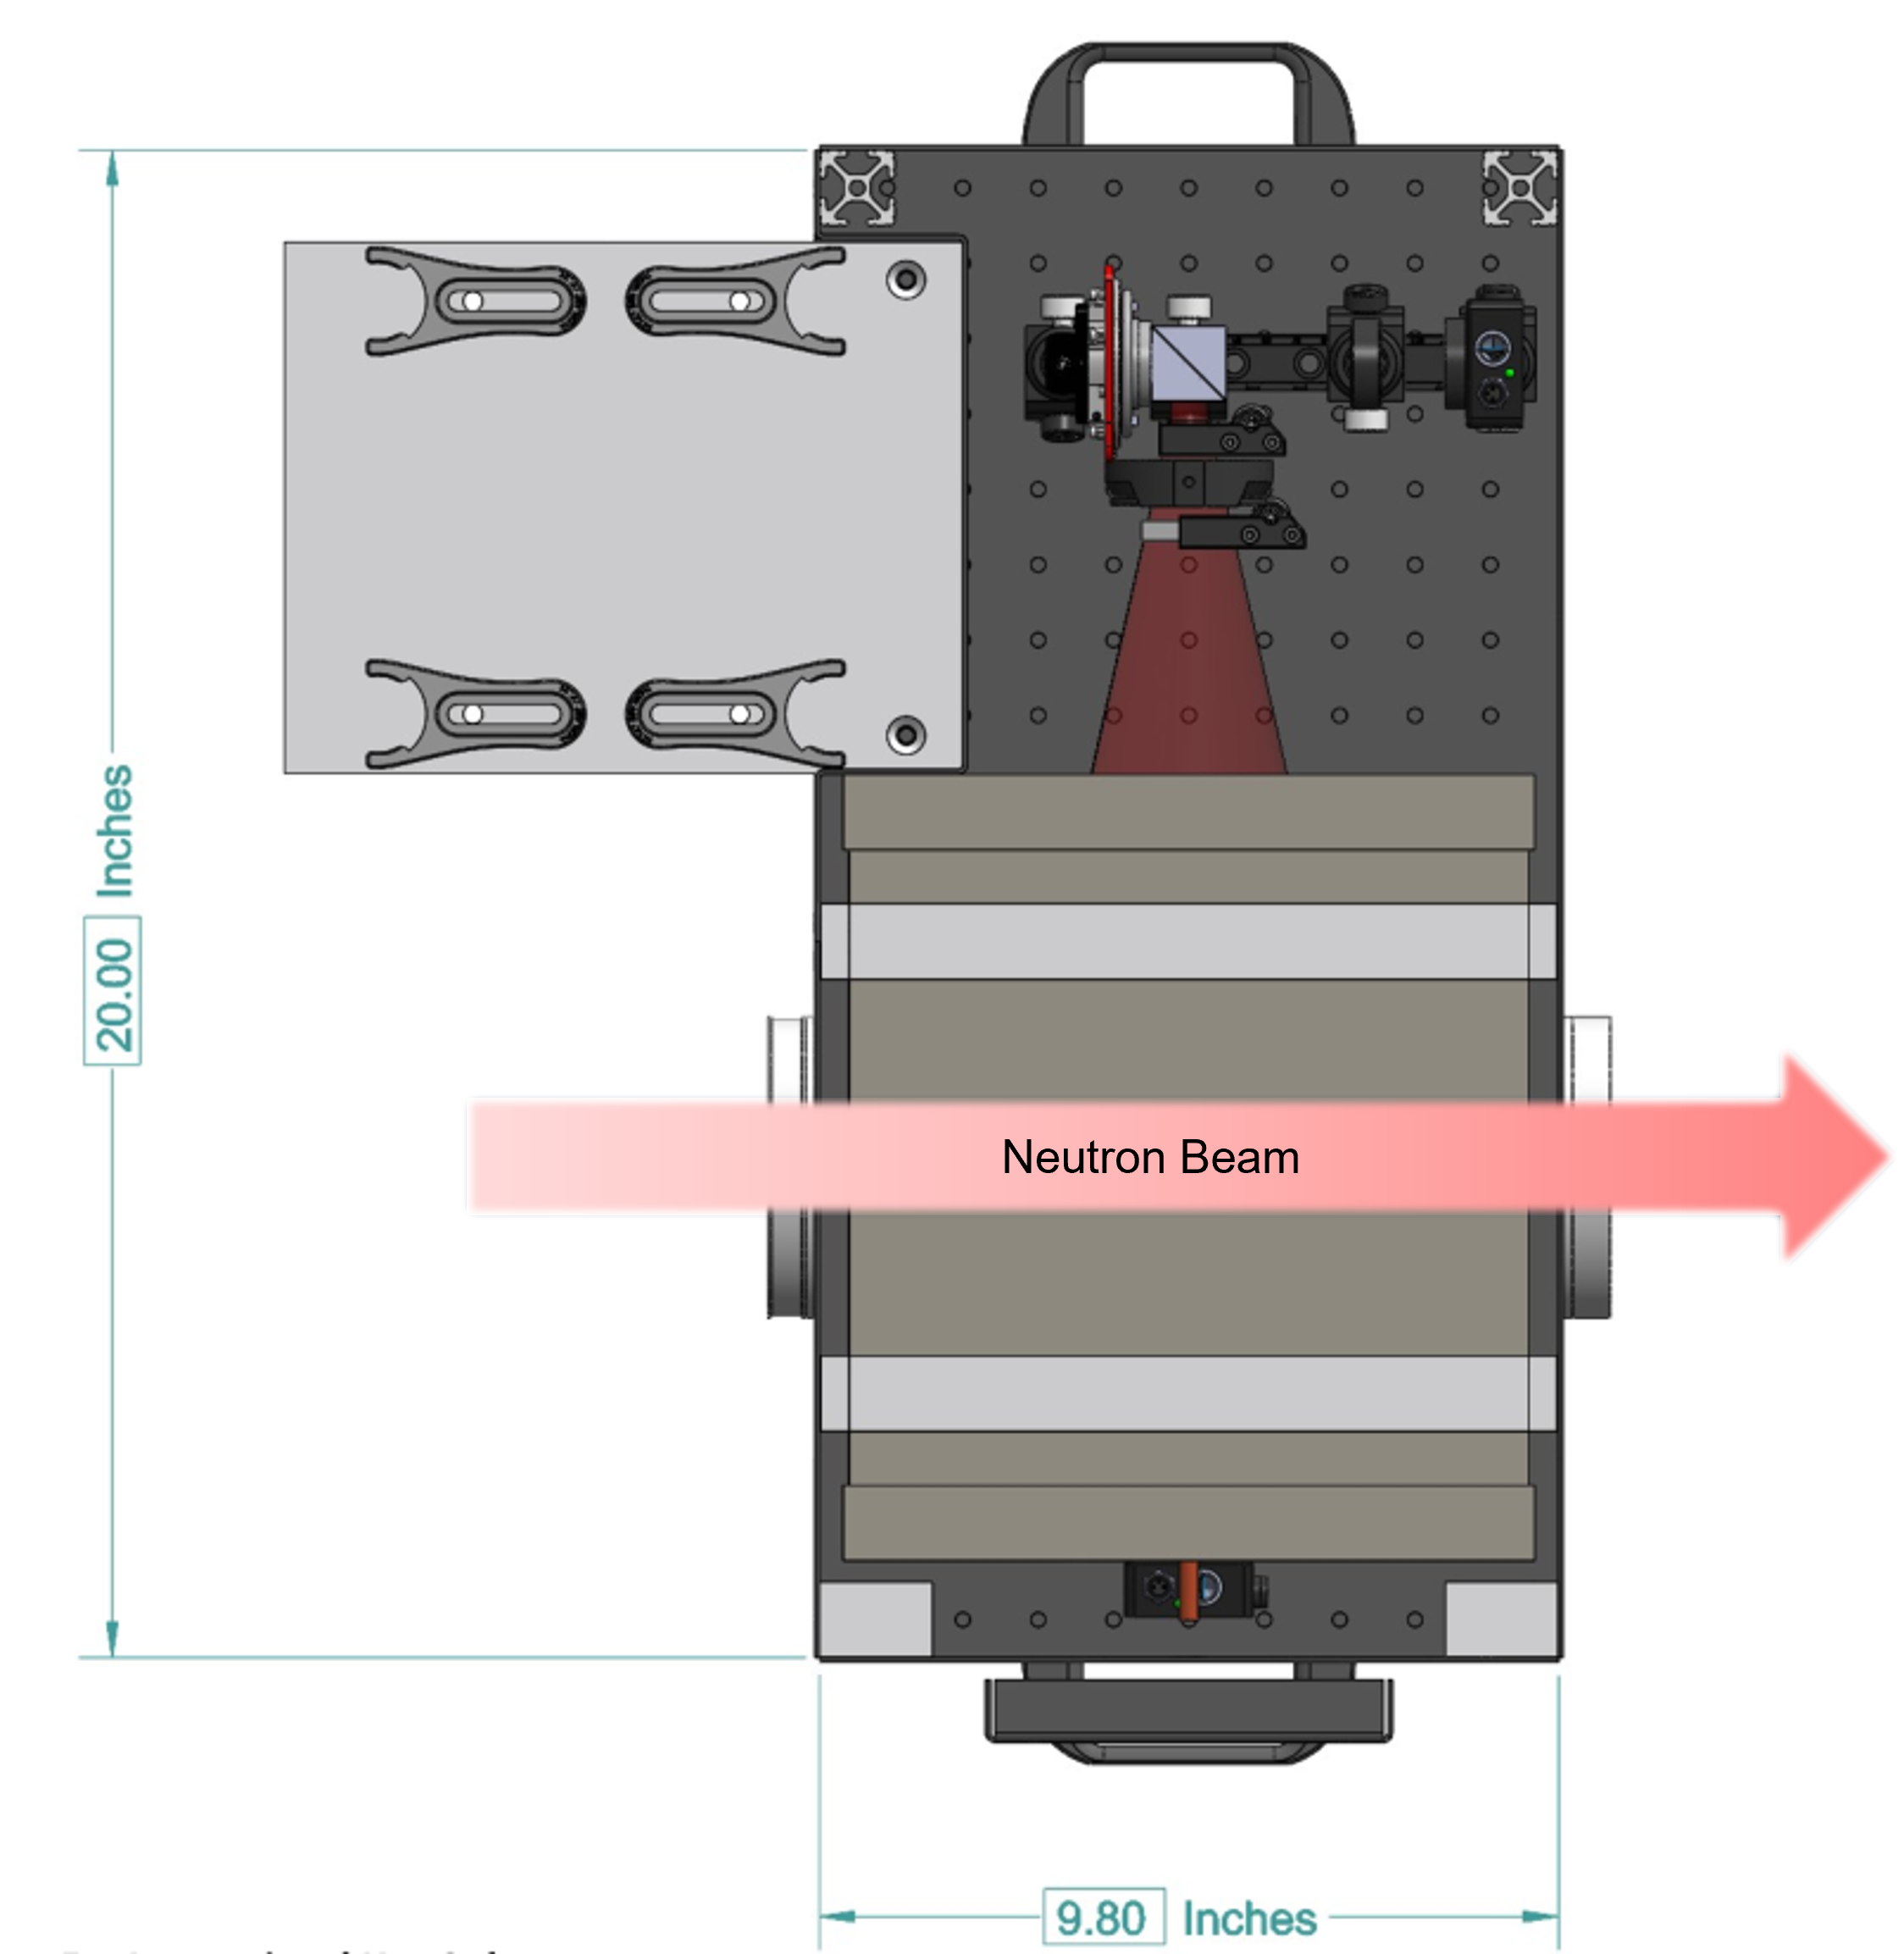
\includegraphics[width=0.8\textwidth, height=0.45\textheight]{figures/chapter3-figs/insitumodel_topdown.png}
         \caption{Top down view.}
         \label{fig:insitu_topdown}
     \end{subfigure}

    \caption{A CAD model of the in situ SEOP system with the major components highlighted.}
    \label{fig:insitumodel}
\end{figure}
\clearpage}

\afterpage{
\begin{figure}
    \centering
    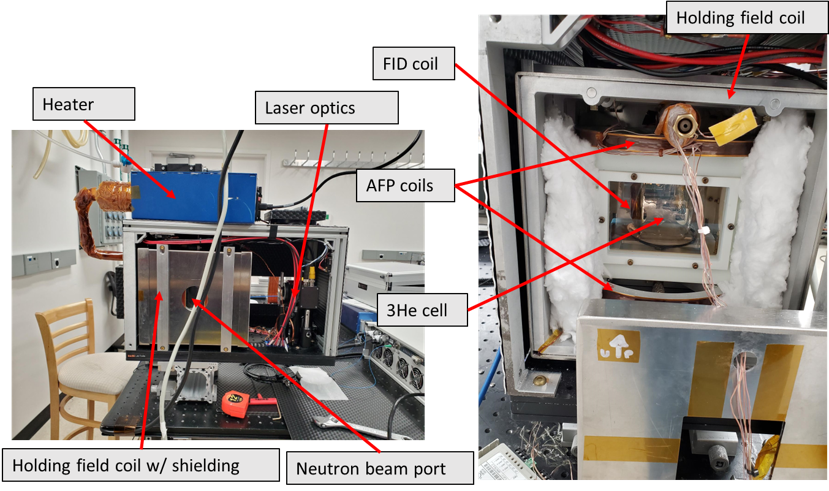
\includegraphics[width=\textwidth]{figures/chapter3-figs/insitupic.png}
    \caption{The in situ $^3$He polarization SEOP system built for the neutron polarimetry experiment conducted in this thesis.}
    \label{fig:insitupic}
\end{figure}
\clearpage}

\subsection{Cell Production}

The $^3$He cell used for this experiment is named “Soccer”. Soccer is made of aluminosilicate glass, GE180, as per the benefits mentioned earlier in this chapter. Soccer has an outer diameter of 7.58 cm and an outer length of 6.62cm. Soccer is placed inside the oven of the in situ SEOP system such that the neutron beam goes along the length of the cell, as illustrated in \cref{fig:insitumodel} and \cref{fig:insitupic}. Soccer was made by the ORNL's glass blowing workshop from GE180 stock. The cell was then installed on the SNS $^3$He filling station \cite{Jiang2013}. It was filled with 0.8bar of $^3$He and 0.08 bar of N$_2$ at room temperature, making it ideal for long wavelength neutron beam polarization measurements. Soccer was built as a hybrid cell with a mixture of Rb and K.

\afterpage{
\begin{figure}
    \centering
    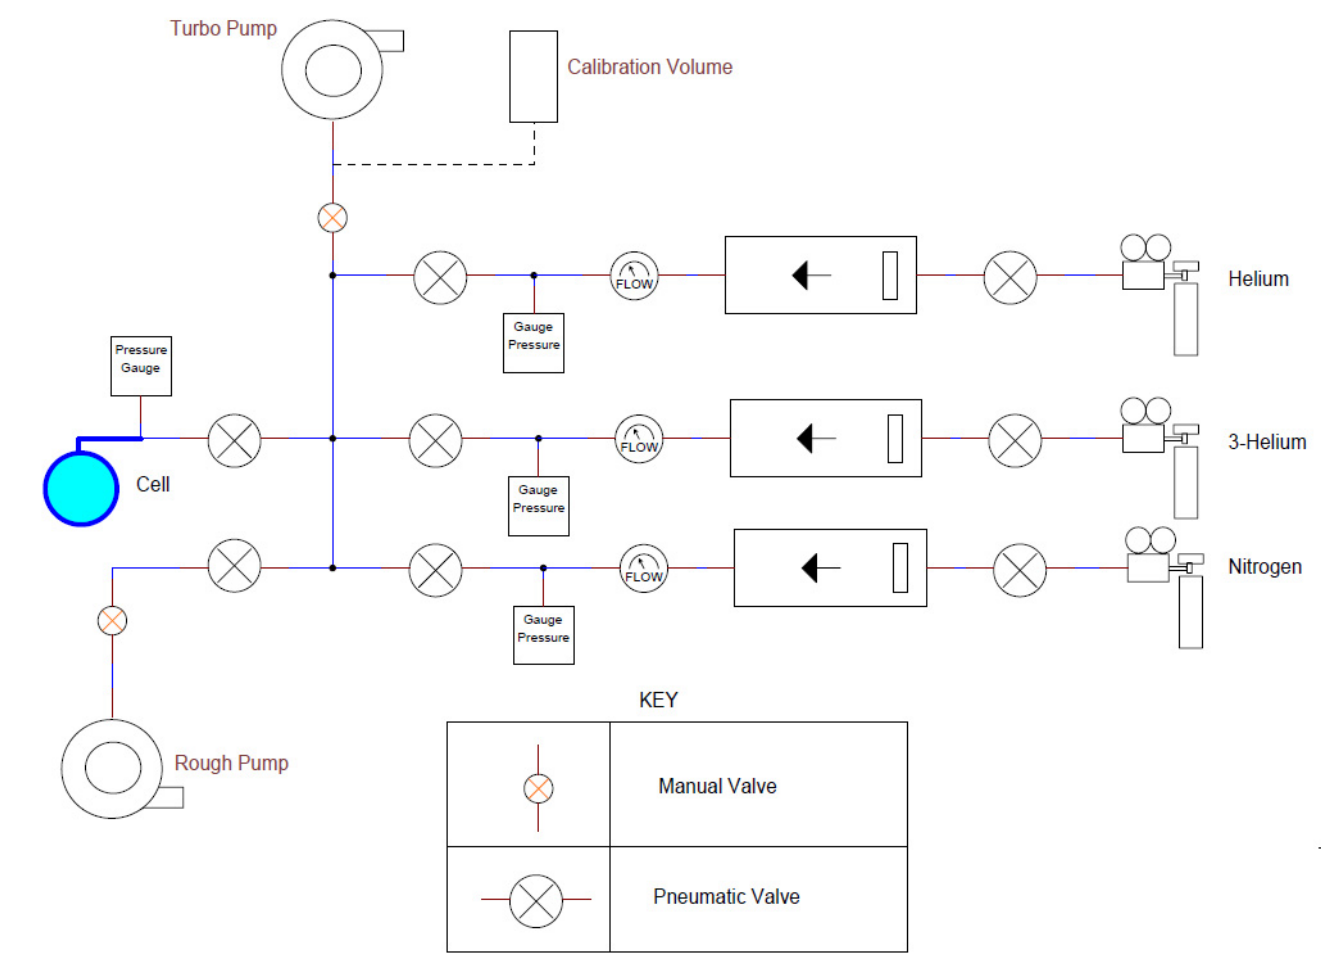
\includegraphics[width=\textwidth]{figures/chapter3-figs/3Hefillingstation.png}
    \caption[Schematic of the SNS $^3$He cell filling station.]{Schematic of the SNS $^3$He cell filling station. Figure taken from \cite{Jiang2013}}
    \label{fig:fillingstation}
\end{figure}
\clearpage}

The glass cell filling is based on the recipe developed by the $^3$He polarization group at National Institute of Standards and Technology (NIST) \cite{Chen2011}. For the first key step, a new cell is thoroughly cleaned prior to filling in order to remove impurities, which can cause a breakdown of SEOP \cite{Chen2011, Jiang2013}. The glass cell stringer assembly is attached to the filling station, as shown in  \cref{fig:fillingstation}, and alkali capsules are dropped into the end tubes, which are then sealed off. The cell is baked at 400 \degree C for two days. A turbo pump is used to pump on the baking cell until high vacuum ($ \sim 10^{-9}$ Torr) is reached. The mass spectrum from Residual Gas Analyzer is also monitored. The key during bake off is to remove any residual water content. After baking, the alkali metals in the capsules are boiled using a flame torch and slowly driven into the cell volume. The alkali mixture ratio is very important for hybrid SEOP as explained earlier in this chapter. A white light halogen lamp and a spectrometer are used to measure the relative intensity of the alkali D1 and D2 absorption lines to characterize the alkali mixture desired ratio. NIST has found the ratio of 1/7 to 1/20 for [Rb]/[K] to be ideal for high $^3$He density hybrid SEOP cells \cite{Chen2011}. Soccer was filled with a 1 part Rb to 3 part K ratio because of its low $^3$He density.

After the alkali filling, the cell gets filled with $^3$He and N$_2$. The gas filling takes place with the filling station shown in \cref{fig:fillingstation}. It consists of a N$_2$ line, a ultra high purity (99.999\%) $^3$He line. The cells are filled with N$_2$ first and then $^3$He. After filling, the cell is closed off from the filling station and separated using a flame torch around the stem of the cell to the stringer assembly. Care is taken to ensure no air leaks in during separation. The pressure in the stringer is recorded using the pressure gauges prior to tip off. Using a calibrated volume, the volume of the new cell is obtained. Thus, the final $^3$He pressure in the cell at room temperature is determined using the ideal gas law. The true cell pressure is determined later from neutron attenuation measurements.

\subsection{Magnetostatic Cavity}

\afterpage{
\begin{figure}
    \centering
    \begin{subfigure}[c]{0.75\textwidth}
        \centering
         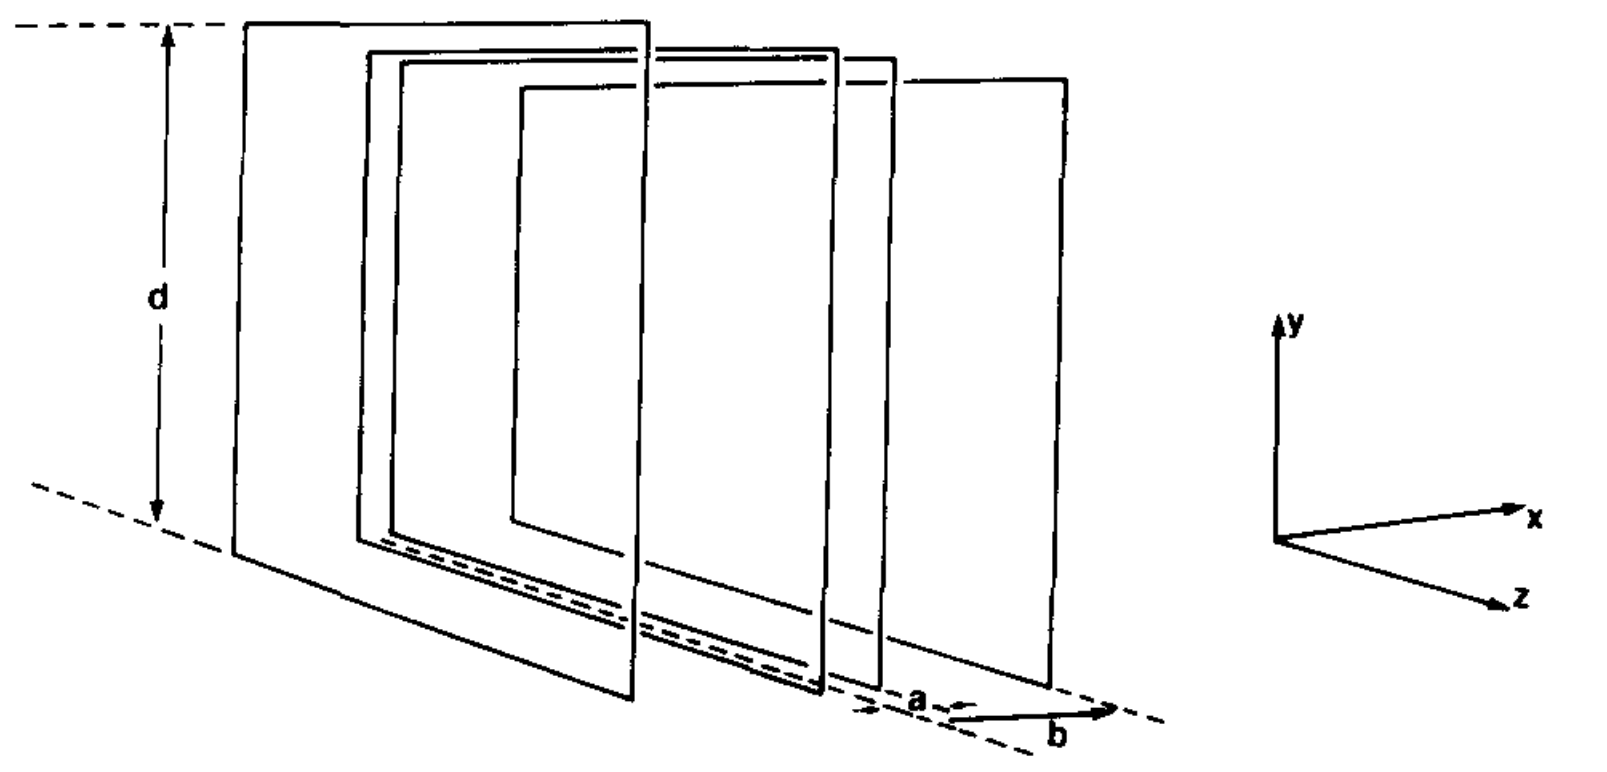
\includegraphics[width=\textwidth]{figures/chapter3-figs/MerrittCoilSchematic.png}
         \caption{A schematic of the four-coil system.}
         \label{fig:Merrittscheme}
     \end{subfigure}
     \hfill
     \begin{subfigure}[c]{0.5\textwidth}
        \centering
         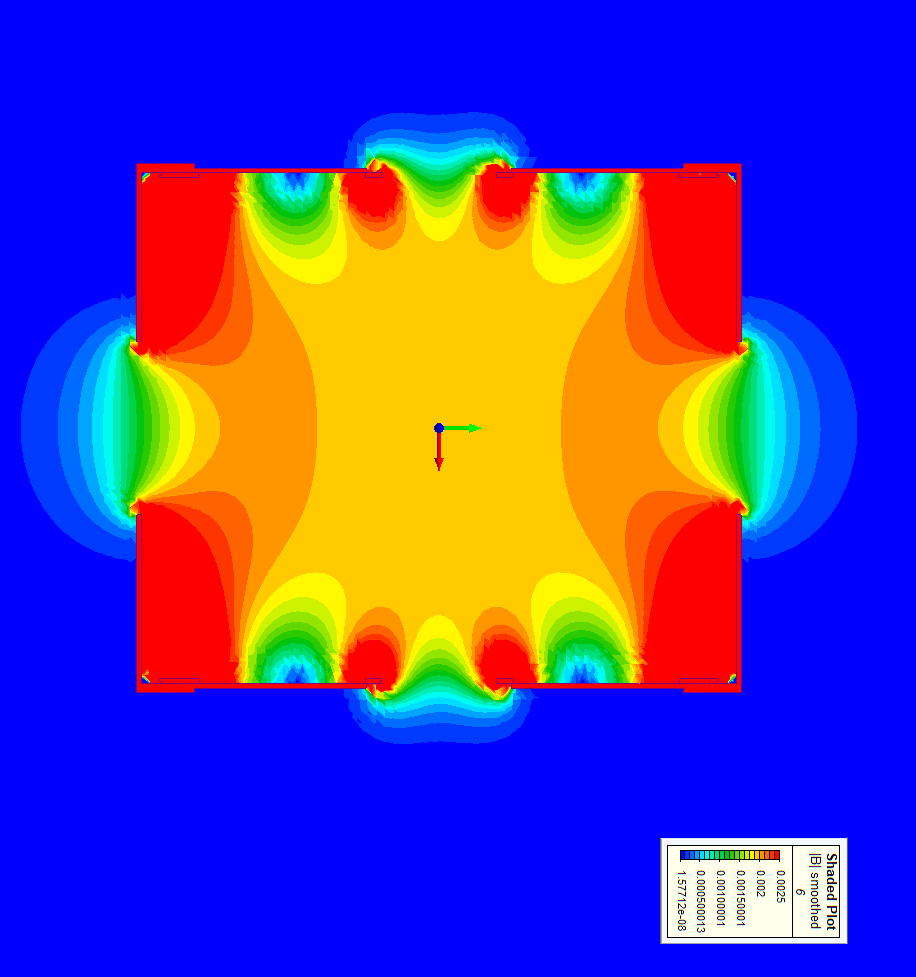
\includegraphics[width=\textwidth]{figures/chapter3-figs/insitumerrittcoil_gradient.png}
         \caption{Simulated magnetic field profile of the four-coil system.}
         \label{fig:Merrittfield}
     \end{subfigure}

    \caption[Merritt's four-coil geometry]{Merritt's four-coil geometry proposed in \cite{Merritt1983}. (b) shows the finite element simulations of the magnetic field profile produced by the 4-coil geometry of the in situ system.}
    \label{fig:Merritt}
\end{figure}
\clearpage}

As described earlier, the $^3$He cell needs to operate in a magnetic holding field in order to define a reference for the polarization. This holding magnetic field also must satisfy the low magnetic fields gradient requirements to prevent $^3$He relaxation. In the in situ system, the holding magnetic field is provided by the four-square coil configuration proposed in \cite{Merritt1983}, a schematic of which is shown in \cref{fig:Merrittscheme}. This four square coil geometry creates a uniform magnetic field for the cell by satisfying:
\begin{itemize}
    \item ratio of the distance, $a$, from the center of the four coils to the inner pair of coils and, $d$, the side length of the coils as $\frac{a}{d} = 0.128$ \cite{Merritt1983}.
    \item ratio of the distance, $b$, from the center to the outer pair of coils and, $d$, as $\frac{b}{d} = 0.505$ \cite{Merritt1983}.
    \item ratio of the current in the inner coil pair, $I_{in}$, to that in the outer coil pair, $I_{out}$, is $\frac{I_{in}}{I_{out}} = 0.423$ \cite{Merritt1983}.
\end{itemize}  
Finite element simulations, as shown in \cref{fig:Merrittfield}, were performed to determine the best winding and current configuration to achieve low gradient magnetic field. For further uniformity and shielding from external fields, which can cause polarized $^3$He relaxation, a rectangular mu-metal magnetic shielding box is used to envelope the four-coil system. \Cref{fig:insitumodel} shows the a model of the four coils and the mu-metal shield inside the in situ enclosure. For the in situ system, the coil was wound with 18AWG wire, with 33 loops in each of the outer coils and 14 loops in each of the inner coils. The outer coils were connected in series with each other and powered to 2.4 Amps. The inner coils were also connected in series with each other and powered at 4.5 Amps. When fully powered, the magnitude of holding magnetic field produced by the full four-coil system along its longitudinal axis is 12.7 Gauss.

\subsection{Oven and Heating System}

The $^3$He cell must be heated in order to vaporize the alkali mixture inside the cell to initiate the SEOP process. \Cref{fig:insitumodel} shows the oven of the in situ system to accommodate the cell. The oven is made of Silicon based fiberglass, capable of 220 \degree C. All sides (except the top and bottom) of the oven have a fused silica windows, which are transparent to neutrons as well as the laser light. The cell is heated by compressed air coming from a heater, flowing in to the oven chamber via an inlet. The cell sits on a pedestal in the center of the oven.

The heater is operated via a PID controller which allows for monitoring and controlling of the heater’s steady state operation. The heater uses incoming compressed air from the facility at 50 psi and heats it with a 1000 W resistive cable, coupled with a flow feedback switch to ensure air flow. Oven temperature is monitored via two thermocouple sensors, one mounted directly on the oven wall. 

\subsection{Laser and Optics}

The laser selected for in situ $^3$He SEOP system is a 50 W 770 nm narrowband laser with a spectral linewidth of 0.2 nm for the D1 transition pumping of K. The laser operates at 47.5 Amp current and the internal laser diode and variable bragg grating are kept cool using a coolant based chiller. Laser head mounts directly to the in situ system as as shown in \Cref{fig:insitumodel}. In order to optically pump the cell, the high-powered infrared light needs to be circularly polarized to match the D1 line of the alkali. This is done by the laser light going through a series of light polarizing optical components. These are shown in \cref{fig:lasersetup}. 

As shown in \cref{fig:lasersetup}, a rotatable half-wave plate (HWP) and polarizing beam splitter (PBS) are used to linearly polarize and reflect the laser beam. The laser beam emerging from the laser head typically has an 80\% linear polarization. By optimizing the half-wave plate rotation, the maximum intensity of the linearly polarized (s-polarized) light is reflected towards the $^3$He cell by the PBS, while the low intensity (p-polarized) transmitted light is dumped into a light diffuser. The half wave plate optimization at low laser power is shown in \cref{fig:HWP}. This optimization was performed by placing a power meter in place of the diffuser and measuring the incident power as a function of half wave plate rotation. The figure shows that the maximum laser was reflected at 70$\degree$ rotation. This half-wave plate setting ensures that the maximum intensity of polarized laser light is incident on the $^3$He cell as well as the liquid crystal retarder. 

The Liquid Crystal Retarder (LCR), acting like a quarter-wave plate, circularly polarizes the incoming linearly polarized laser beam. The LCR works by applying a voltage through the liquid crystal to alter the birefringence and hence inducing a polarization phase shift to circularly polarize the light. The LCR voltage was tuned to induce both the left-handed ($\sigma_-$) and right-handed ($\sigma_+$) circularly polarized light by measuring the laser polarization using an optical polarimeter. The best possible degree of circular polarization, 80.3\% ($\sigma_-$) and 82.6\% ($\sigma_+$), observed at LCR voltage settings, 3.13 V for ($\sigma_-$) and 2.17 V ($\sigma_+$), respectively, is shown in \cref{tab:docp}. These LCR settings were used during the SEOP operation, 3.13V for polarizing $^3$He parallel to the holding magnetic field and 2.17V for polarizing $^3$He antiparallel to the holding magnetic field. Both the half wave plate and the LCR can be tuned remotely.

\afterpage{
\begin{figure}
    \centering
    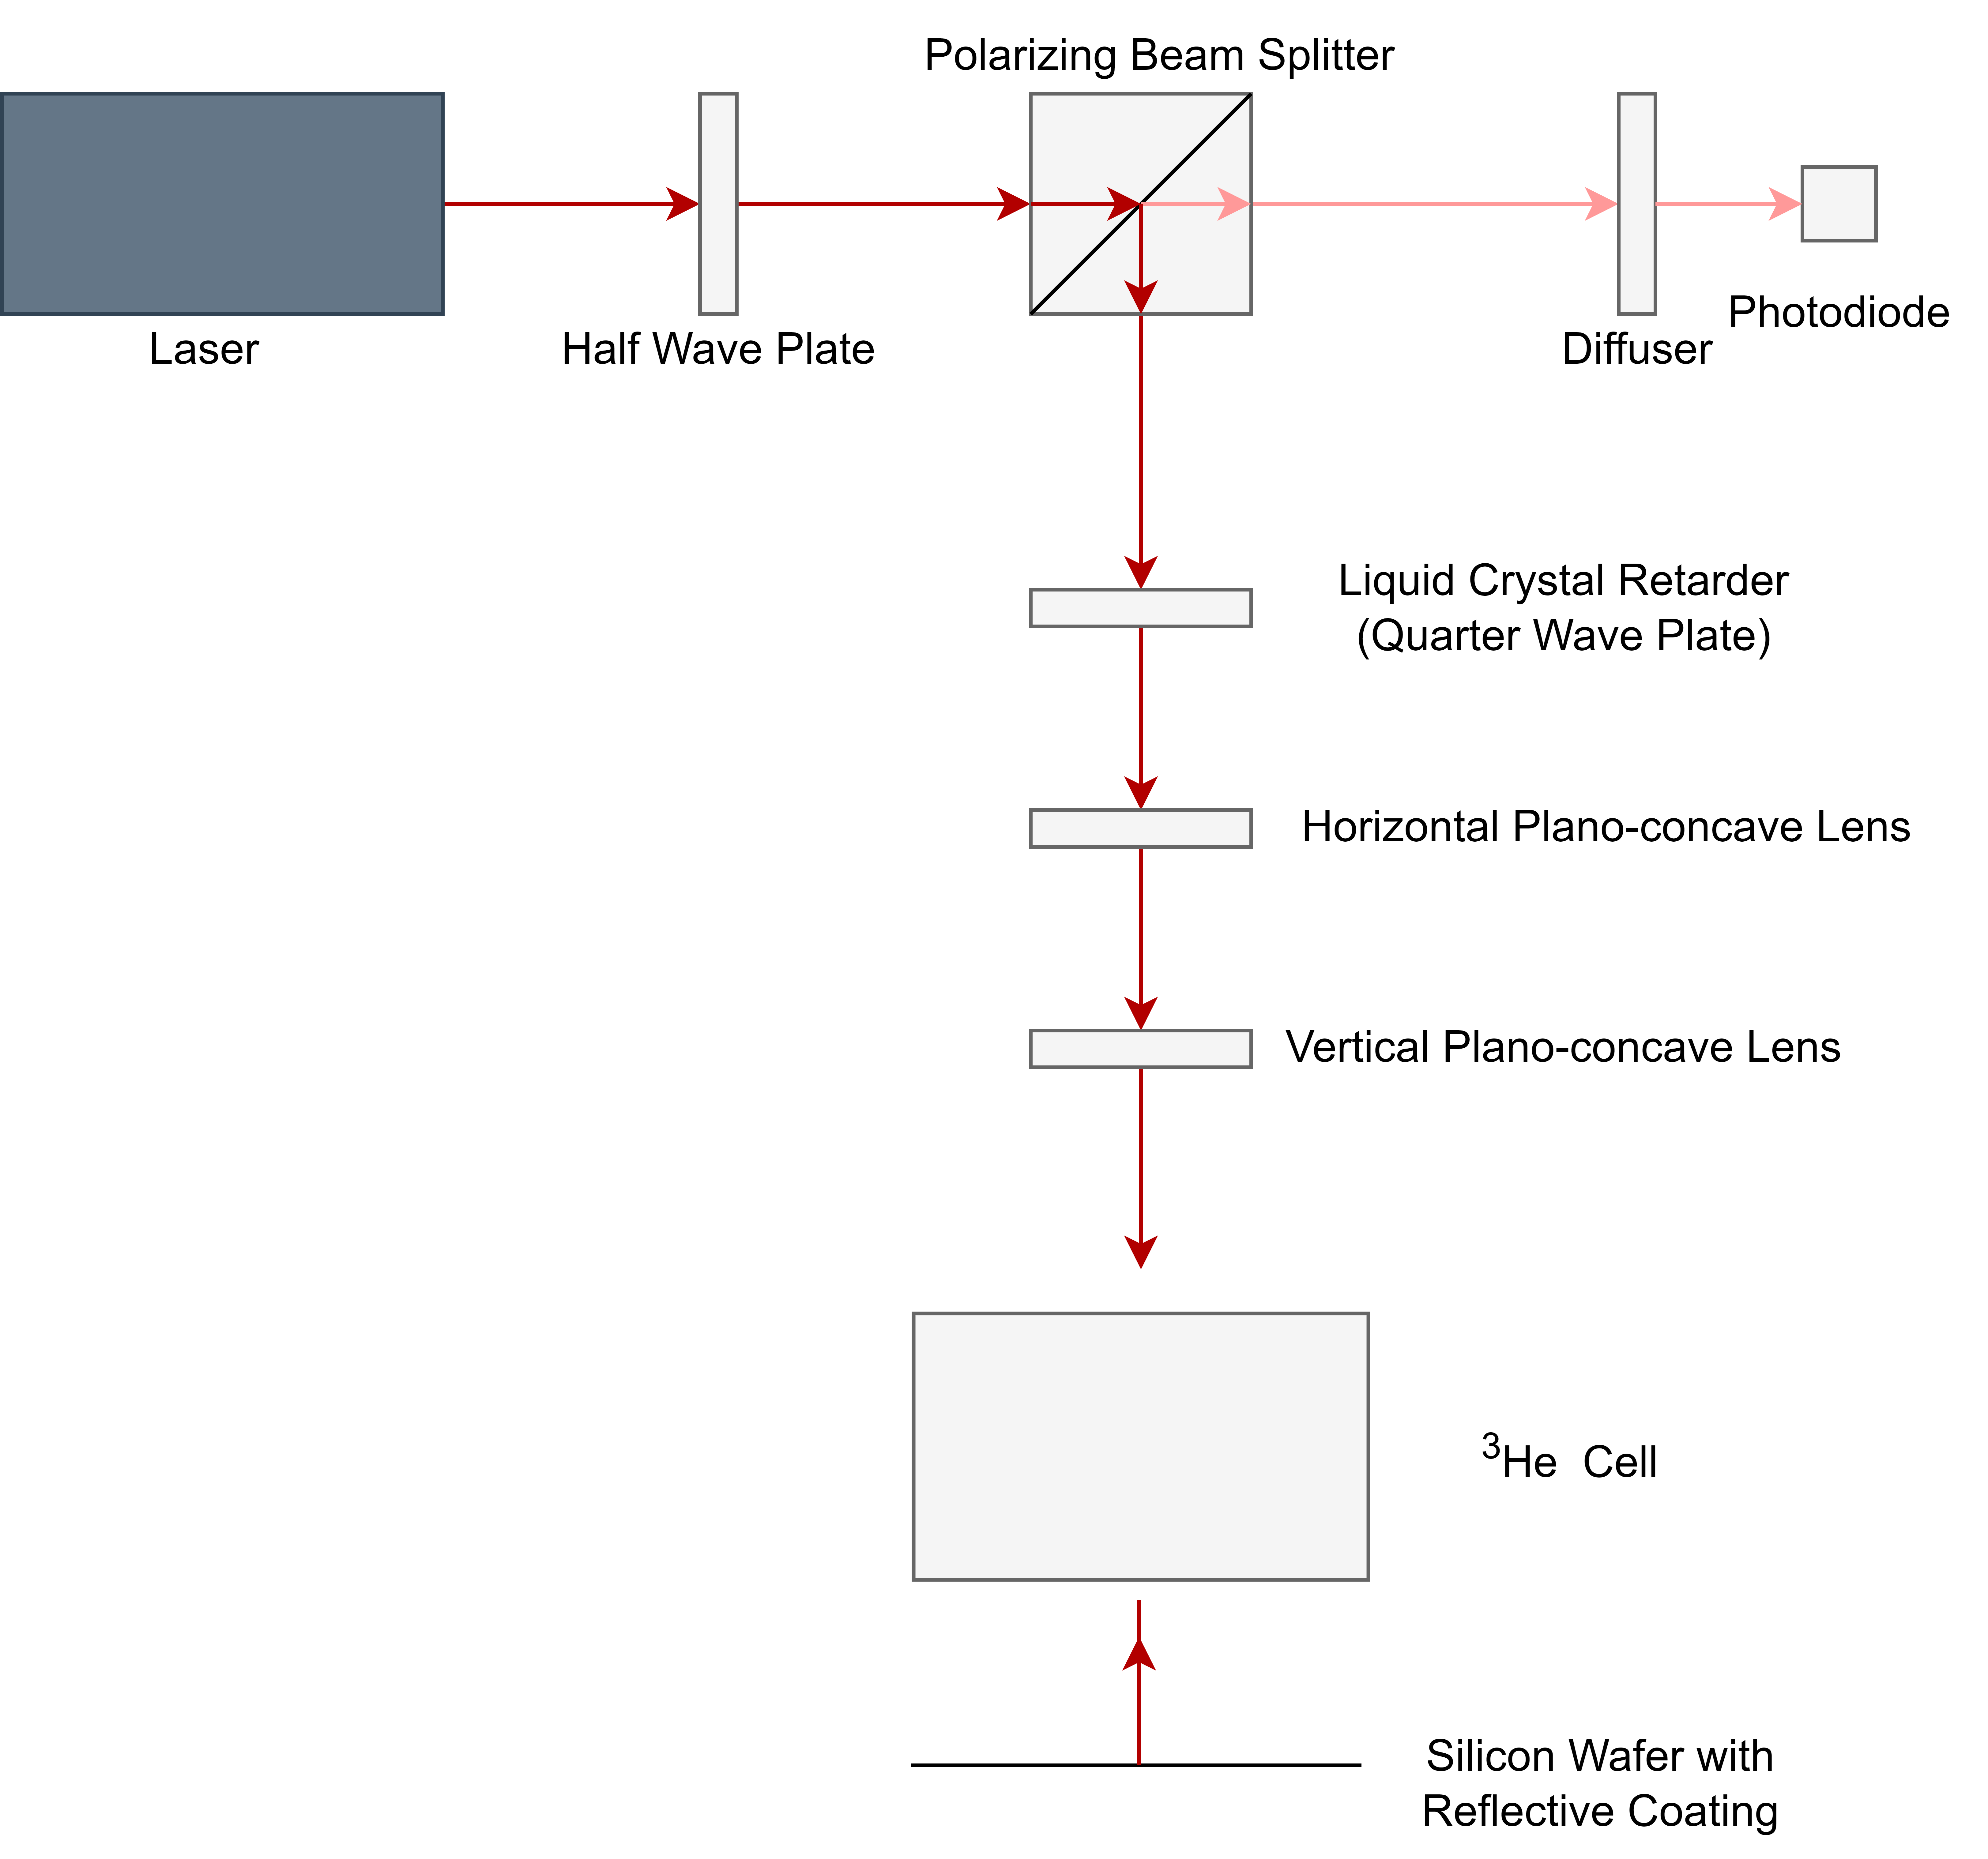
\includegraphics[width=\textwidth]{figures/chapter3-figs/In-situSEOPlaser.png}
    \caption{Setup of the laser optics used in the in situ SEOP system.}
    \label{fig:lasersetup}
\end{figure}
\clearpage}

\afterpage{
\begin{figure}
    \centering
    \includegraphics[width=\textwidth]{figures/chapter3-figs/HWPoptimization.png}
    \caption{Optimization of the half wave plate at 5 A laser power. The trend shows the change in transmitted power as a function of the rotation of the HWP i.e. it's birefringence.}
    \label{fig:HWP}
\end{figure}
\clearpage}

\afterpage{ 

\begin{table}
\centering
\centering
\begin{threeparttable}
\caption{Measured degree of circular polarization of the laser from the liquid crystal retarder acting as a quarter wave plate.}
\label{tab:docp}
\begin{tabular}{@{}cccc@{}}
\toprule
LCR Voltage [V] & Circularly Polarized Light Orientation & DOCP\tnote{*} & DOLP\tnote{**} \\
\midrule
2.17 & Left & 80.47\% & 3.58\% \\
3.13 & Right & 82.17\% & 4.28\% \\
\bottomrule
\end{tabular}

    \begin{tablenotes}
      \item[*] Degree of Circular Polarization
      \item[**] Degree of Linear Polarization
    \end{tablenotes}

  \end{threeparttable}
\end{table}

\clearpage}

The circularly polarized light goes through a series of vertical and horizontal plano-concave lenses to expand the beam spot size so that the entire $^3$He cell is illuminated. An Infrared light sensitive laser phosphor card was used to ensure the full coverage of the cell by the laser light. Even though the laser beam is being applied from oneside to keep the system as compact as possible, a silicon wafer with a reflective coating was placed behind the cell to get double sided laser illumination on the cell.

%\afterpage{
%\begin{figure}
%     \centering
%     \begin{subfigure}{\textwidth}
%         \centering
%         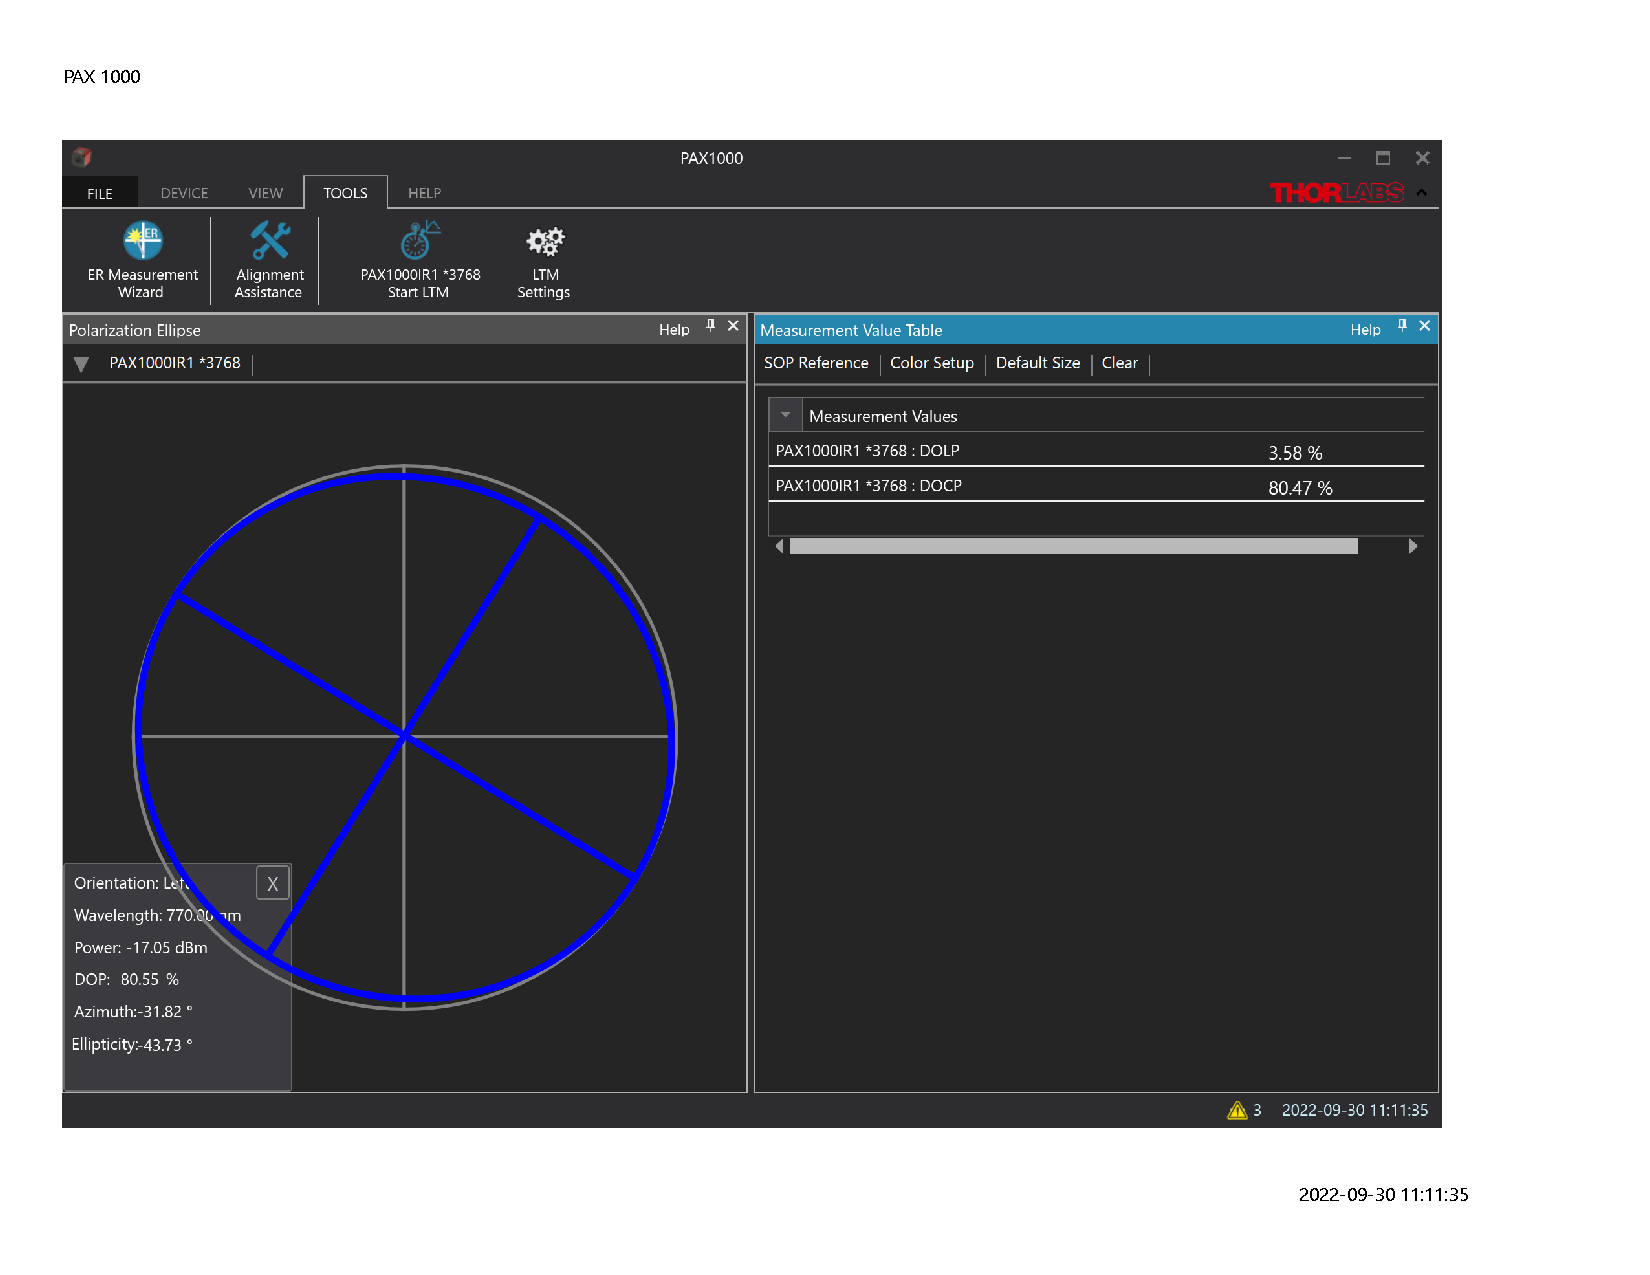
\includegraphics[width=0.7\textwidth]{figures/chapter3-figs/Opt_pol_left.pdf}
%         \caption{Left handed ($\sigma_{-}$) light degree of polarization}
%         \label{fig:leftdop}
%     \end{subfigure}
%     \hfill
%     \begin{subfigure}{\textwidth}
%         \centering
%         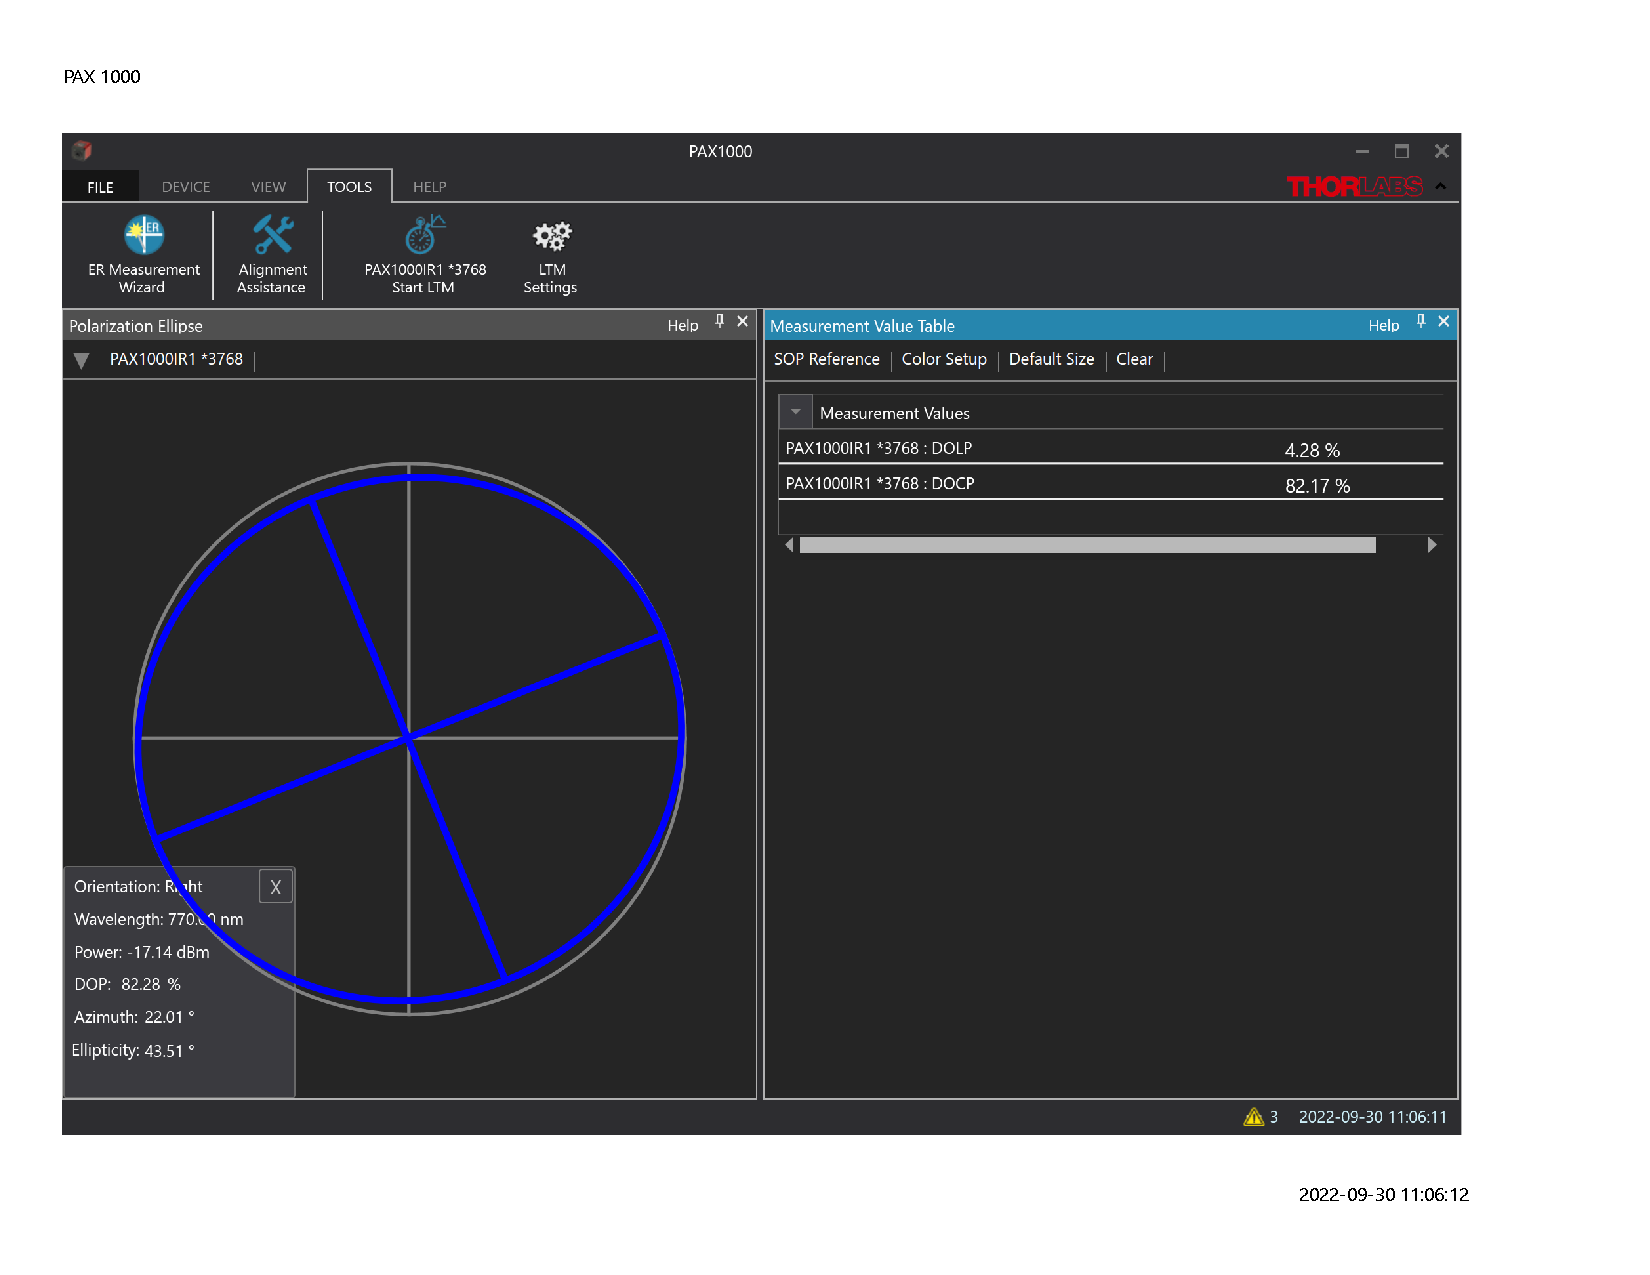
\includegraphics[width=0.7\textwidth]{figures/chapter3-figs/Opt_pol_right.pdf}
%         \caption{Right handed ($\sigma_{+}$) light degree of polarization}
%         \label{fig:rightdop}
%     \end{subfigure}
%        
%        \caption{Measured degree of circular polarization of the laser from the liquid crystal retarder acting as a quarter wave plate.}
%        \label{fig:docp}
%
%\end{figure}
%\clearpage}

Since the in situ system was to be operated at a beamline and not a designated laser laboratory, the laser must operate as a Class 4 embedded Class 1 configuration to comply with the safety guidelines of the SNS. The in situ system laser was interlocked with the side enclosure panels using limit switches. Tampering of the enclosure during laser operations would trigger the limit switches and the laser would be de-energized instantly. This feature ensures the safety of the personnel working in close proximity to the in situ system under a fault scenario. This feature also simplified the experimental setup, by eliminating the need for light tight barriers/curtains and laser safety PPE.


\section{Characterization and Control of $^{3}$He Polarization}

There are three widely used methods to monitor and manipulate the $^3$He polarization of $^3$He cells: Nuclear Magnetic Resonance (NMR) Spectroscopy \cite{Lorenzon1993, Romalis1998}, Electron Paramagnetic Resonance (EPR) Spectroscopy \cite{Romalis1998, Babcock2005} and neutron transmission \cite{Jones2000, Chupp2007}. For the in situ system, an NMR system capable of both Free Induction Decay (FID) and Adiabatic Fast Passage (AFP) techniques as well as an EPR system was built. This section will describe them and their use in performance testing of the in situ system.

\subsection{Nuclear Magnetic Resonance Spectroscopy}

Technically, EPR and neutron transmission provide an absolute measurement of the $^3$He polarization. However, NMR can still be used as diagnostic tool for monitoring/manipulating the $^3$He polarization, spin up time and $T_1$ time as well as to measure the relative magnetic field gradients, albeit only to optimize the magnetic field environment rather than as an absolute magnetometer. This section describes the FID and AFP NMR setup used in the in situ system.

\subsubsection{Free Induction Decay}

The relative $^3$He polarization is typically monitored by FID NMR \cite{Bloch1946, Abragam1961}. In FID NMR, a small pickup coil mounted on the $^3$He cell is used to apply a RF pulse to slightly tip the $^3$He spins off the Larmor precession. Then, the transverse component of the $^3$He precession relaxing back from the tip towards the longitudinal Larmor precession induces a signal in the pick up for detection. This signal shows the relaxing transverse precession as an decaying oscillation envelope characterized by, $T_2^*$, the transverse polarization relaxation time, given as
\begin{equation}
    \frac{1}{T_2^*} = \gamma_3 \Delta B_0
\end{equation}
where $\gamma_3$ is the $^3$He's gyromagnetic ratio and $\Delta B_0$ is presence of gradients over the portion of $^3$He polarization volume sampled by the coil. $T_2^*$ is representative of fluctuations in spin precession from magnetic-field inhomogeneities.

This magnetization measurement approach is mostly nondestructive since small tip angles are used from a pickup coil of size smaller than the cell \cite{Lorenzon1993, Parnell2008, Chen2011}. $T_2^*$ is typically on the order of milliseconds, where longer $T_2^*$ means smaller magnetic field gradients, $\Delta B_0$ \cite{Lorenzon1993,  Parnell2008, Chen2011}.

For the in situ system, the FID coil is a circular coil, about 1 inch in diameter, with 150 loops of 0.0093 inch diameter copper wire, taped to the cell. The total coil resistance is 2.6 $\Omega$. The coil applies a RF pulse of 1.5 ms duration and 10 V amplitude orthogonal to the holding field, $B_0$. The short pulse duration time is necessary for the diabatic field tipping process at the Larmor frequency of 41.16 kHz (12.7 Gauss). Otherwise, the $^3$He spins can get adiabatically locked to the tipping field plus holding magnetic field $B_0+B_{RF}$ and lose their polarization. The tipping magnetic field leads to a transverse component in the polarization, which induces a voltage (FID signal) in the pickup coil at the rising and falling edge of the $B_{RF}$ pulse. The FID signal consists of the falling edge since there is a low chance of inducing a field gradient some time after $B_{RF}$ was applied, resulting in longer $T_2^*$. 

The FID setup is based on the technique by \cite{Parnell2008} and shown in \cref{fig:NMRsetup}. The signal from the pickup coil is fed into a low pass filter with a transmission/reciever switch, with a high quality factor. Pick up coil is only active when the control software requests an FID signal to prevent a self oscillating circuit, which would degrade $^3$He polarization. The signal after the preamplifier gets fed into digital I/O card [National Instruments USB-6259] with a built-in phase lock-in amplifier. NI USB-6251 DAC board also generates reference frequency signal close to the $^3$He Larmor frequency via an internal phase locked loop. This reference frequency is used to determine the phase of the outgoing waveform signal. The reference frequency was set so the beat frequency of the outgoing signal and the reference signal was in the 100-300 Hz range. The frequency bin width is set at 1 $\mu$Hz to prevent aliasing. 

\afterpage{
\begin{figure}
    \centering
    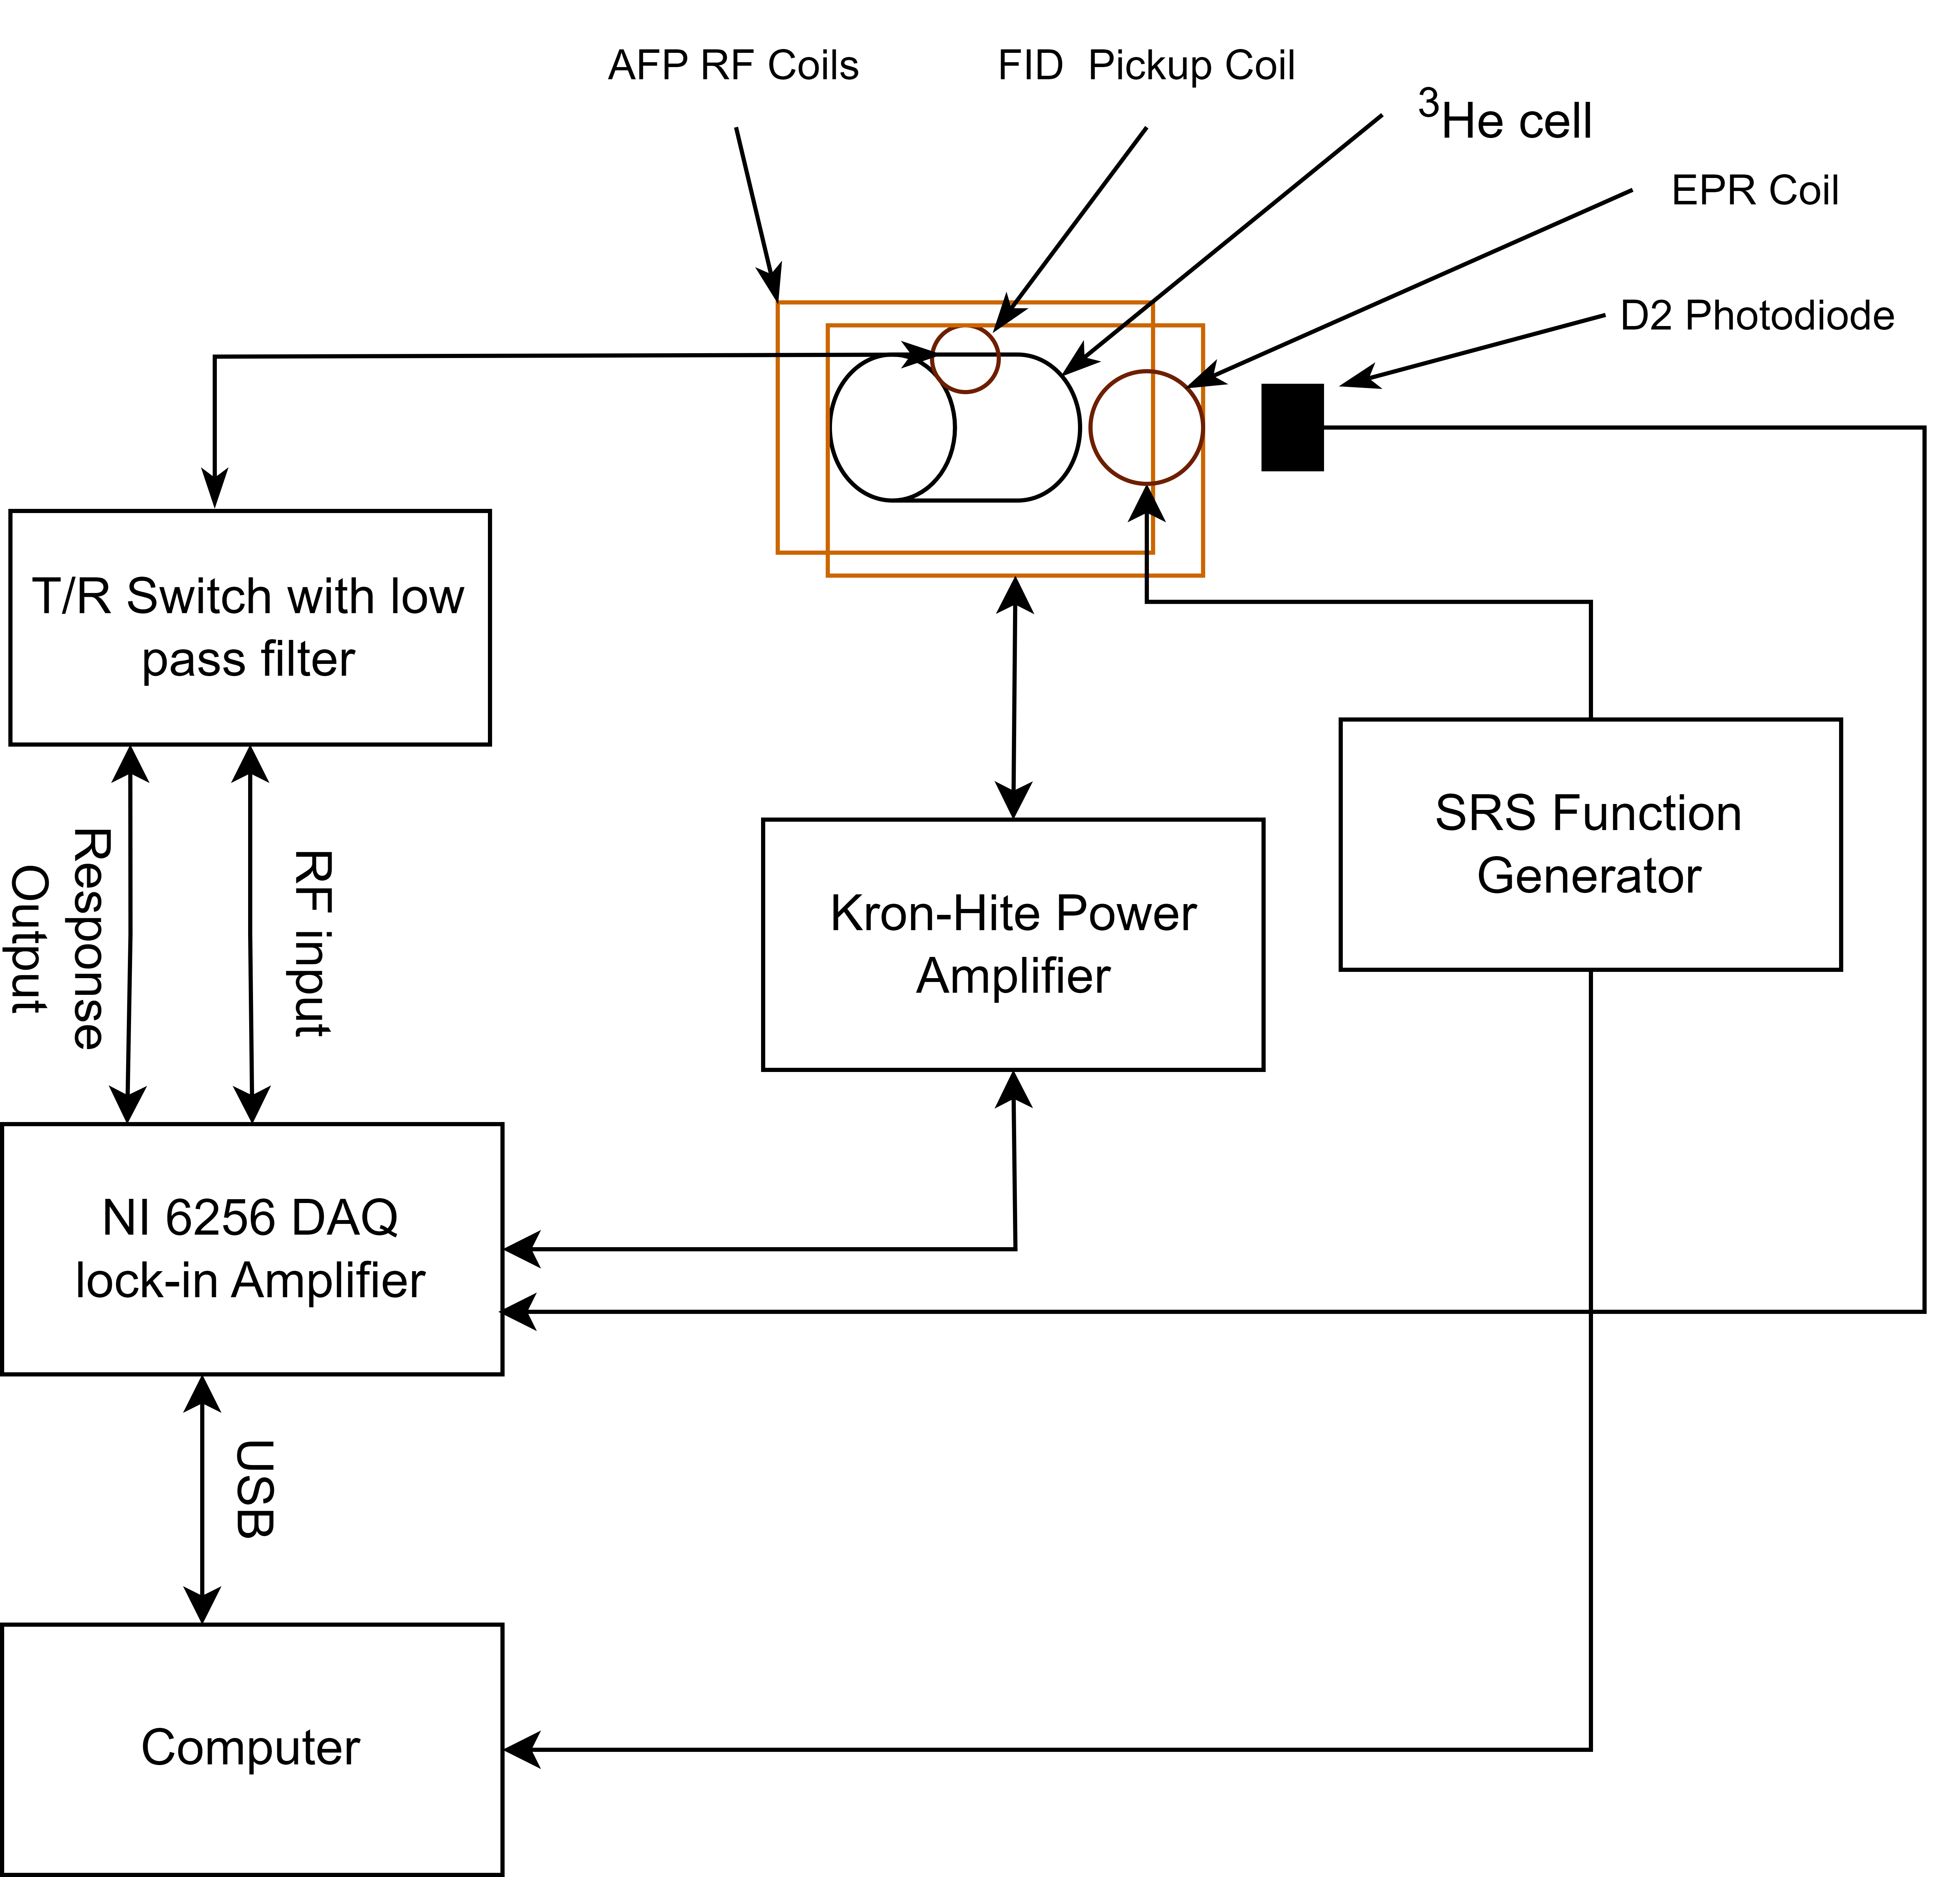
\includegraphics[width=\textwidth]{figures/chapter3-figs/NMRSetup.png}
    \caption[Schematic of the NMR setup used in the in situ SEOP system based on the digitization technique]{Schematic of the NMR setup used in the in-situ SEOP system based on the digitization technique described in \cite{Parnell2008}.}
    \label{fig:NMRsetup}
\end{figure}
\clearpage}

\Cref{tab:FID_params} shows the parameters used to optimize the FID NMR system. \Cref{fig:FIDsignals} shows the raw FID response signal based the parameters in \cref{tab:FID_params}. \Cref{fig:FFTxcomp} and \cref{fig:FIDycomp} shows the decomposed FID signal along with the fit based on: 
\begin{equation}
    f(t) = \frac{1}{2} V_{pp} sin(\omega_L t + \phi) \exp\left( \frac{-t}{T_2^*}    \right)
    \label{eq:FID}
\end{equation}
where $V_{pp}$ is the peak to peak voltage caused by the spin precession tipping from the FID pulse and $\omega_L$ is the Larmor frequency and $\phi$ is the phase of the sinusoidal wave.

\afterpage{
\begin{table}
\centering
\caption{List of parameters used for FID NMR on polarized $^3$He.}
\label{tab:FID_params}
\begin{tabular}{@{}lc@{}}
\toprule
FID Parameters                 & FID Parameter Values \\ 
\midrule
Larmor Frequency {[}Hz{]}      & 41160                \\
Pulse Length {[}sec{]}         & 0.0015               \\ 
RF Amplitude {[}V{]}           & 5-10               \\ 
B-field {[}V{]}                & 2.07               \\ 
Readout Time {[}sec{]}         & 0.08               \\
Additional Mute Time {[}sec{]} & 0.0025               \\
Low pass filter {[}Hz{]}       & 1000               \\
Signal Range {[}V{]}           & 0.1               \\
\bottomrule
\end{tabular}
\end{table}
\clearpage}

\afterpage{
\begin{figure}
    \centering
    \begin{subfigure}[b]{0.5\textwidth}
        \centering
        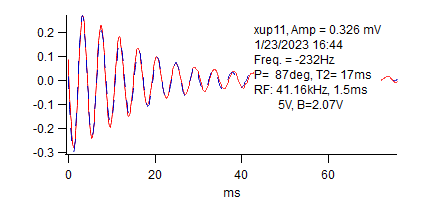
\includegraphics[width=\textwidth]{figures/chapter3-figs/xup_graph.png}
        \caption{x-component of decomposed FID coil response. The units on y-axis are mV.}    
        \label{fig:FFTxcomp}
    \end{subfigure}
    \hfill
    \begin{subfigure}[b]{0.5\textwidth}  
        \centering 
        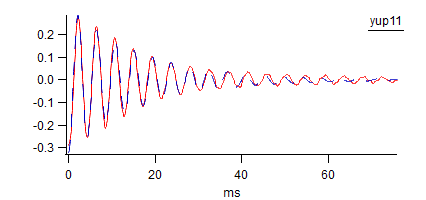
\includegraphics[width=\textwidth]{figures/chapter3-figs/yup_graph.png}
        \caption{y-component of decomposed FID coil response. Notice the 90$\degree$ phase shift with respect to the x-component. The units on y-axis are mV.}    
        \label{fig:FIDycomp}
    \end{subfigure}
    \vskip\baselineskip
    \begin{subfigure}[b]{0.5\textwidth}   
        \centering 
        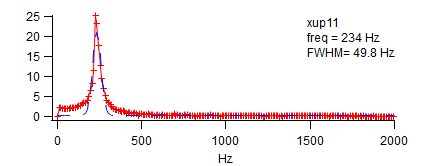
\includegraphics[width=\textwidth]{figures/chapter3-figs/FFT_graph.png}
        \caption{Fast Fourier Transform of the FID coil response.}    
        \label{fig:FIDFFT}
    \end{subfigure}
    \hfill
    \begin{subfigure}[b]{0.5\textwidth}   
        \centering 
        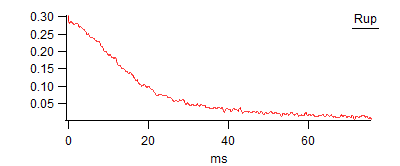
\includegraphics[width=\textwidth]{figures/chapter3-figs/rup_graph.png}
        \caption{A plot of R of FID response. The units on y-axis are mV.}    
        \label{fig:FIDr}
    \end{subfigure}
    \caption{FID response of the polarized $^3$He cell, Soccer. Red curve is the measured response and the blue curve is the fit.}
    \label{fig:FIDsignals}
\end{figure}
\clearpage}

The key indicators from this fit are (i) $T_2^*$ time, which can be used monitor any variations in magnetic field inhomogeneities over time, (ii) the signal amplitude in [mV], which is used to monitor the relative change in $^3$He polarization over time, and (iii) the phase, which can be used to check for polarization inversion by for e.g. as AFP flip or any dephasing due to magnetic field gradients. \cref{fig:FIDFFT} shows the FFT spectrum of the FID response signal. The spectrum peak represents the beat frequency of the larmor precession of the $^3$He polarization and with respect to the reference frequency set by the lock-in amplifier. FFT spectrum can be used to check for sudden or unwanted changes the holding magnetic field, $B_0$. The integral of the FFT spectrum is also proportional to the $^3$He cell polarization, so if the absolute $^3$He polarization is well known, then the integral of the FFT can be used to monitor any changes in absolute $^3$He polarization. In NMR, response signal can be affected by what is known as radiation damping, where different precessions can generate a RF induced current in the coil causing the FID response to be damped \cite{Augustine2002}. It can also happen if the induced FID signal becomes in resonance with the coil. \Cref{fig:FIDr} shows that $R=\sqrt{(x^2 + y^2)}$, where x is the x-comp of FID and y is the y-comp of FID. R in addition to the FFT spectrum can be used to monitor any damping of the FID signal from noise.

\Cref{fig:NMRLoss} shows that the application of a FID pulse sequence results in a relative $^3$He polarization loss of 1-cos($\theta$) = 0.33\% per 5 pulses, corresponding to a tipping angle of $\theta \approx 4\degree$. Due to minimal losses in $^3$He polarization from FID, this NMR monitoring can be utilized in parallel with neutron beam transmission data taking. Even though only a comparative $^3$He polarization is extracted by the FID method, nevertheless, it is useful for monitoring the polarization buildup saturation time as well as the polarization decay ($T_1$ time) i.e lifetime of the $^3$He cell. In \Cref{fig:spinup}, the characteristic time of the fit exponential is called the "spin up time" i.e. the time it takes for $\frac{1}{e}$ population of $^3$He to polarize. The curve plateaus off as time indicating $^3$He cell polarization saturation. For an in situ system, because the $^3$He cell is undergoing continuous optical pumping, this curve should saturate as function of time. In \Cref{fig:spindown}, the characteristic time of this exponential is called the "spin down time" or the $T_1$ time i.e. the time it takes for $\frac{1}{e}$ population of $^3$He to depolarize. Although this time is irrelevant for in situ SEOP systems, courtesy of continuous in situ SEOP polarization, nevertheless, it showcases the longevity of a $^3$He cell polarization in a holding magnetic field.

\afterpage{
\begin{figure}
    \centering
    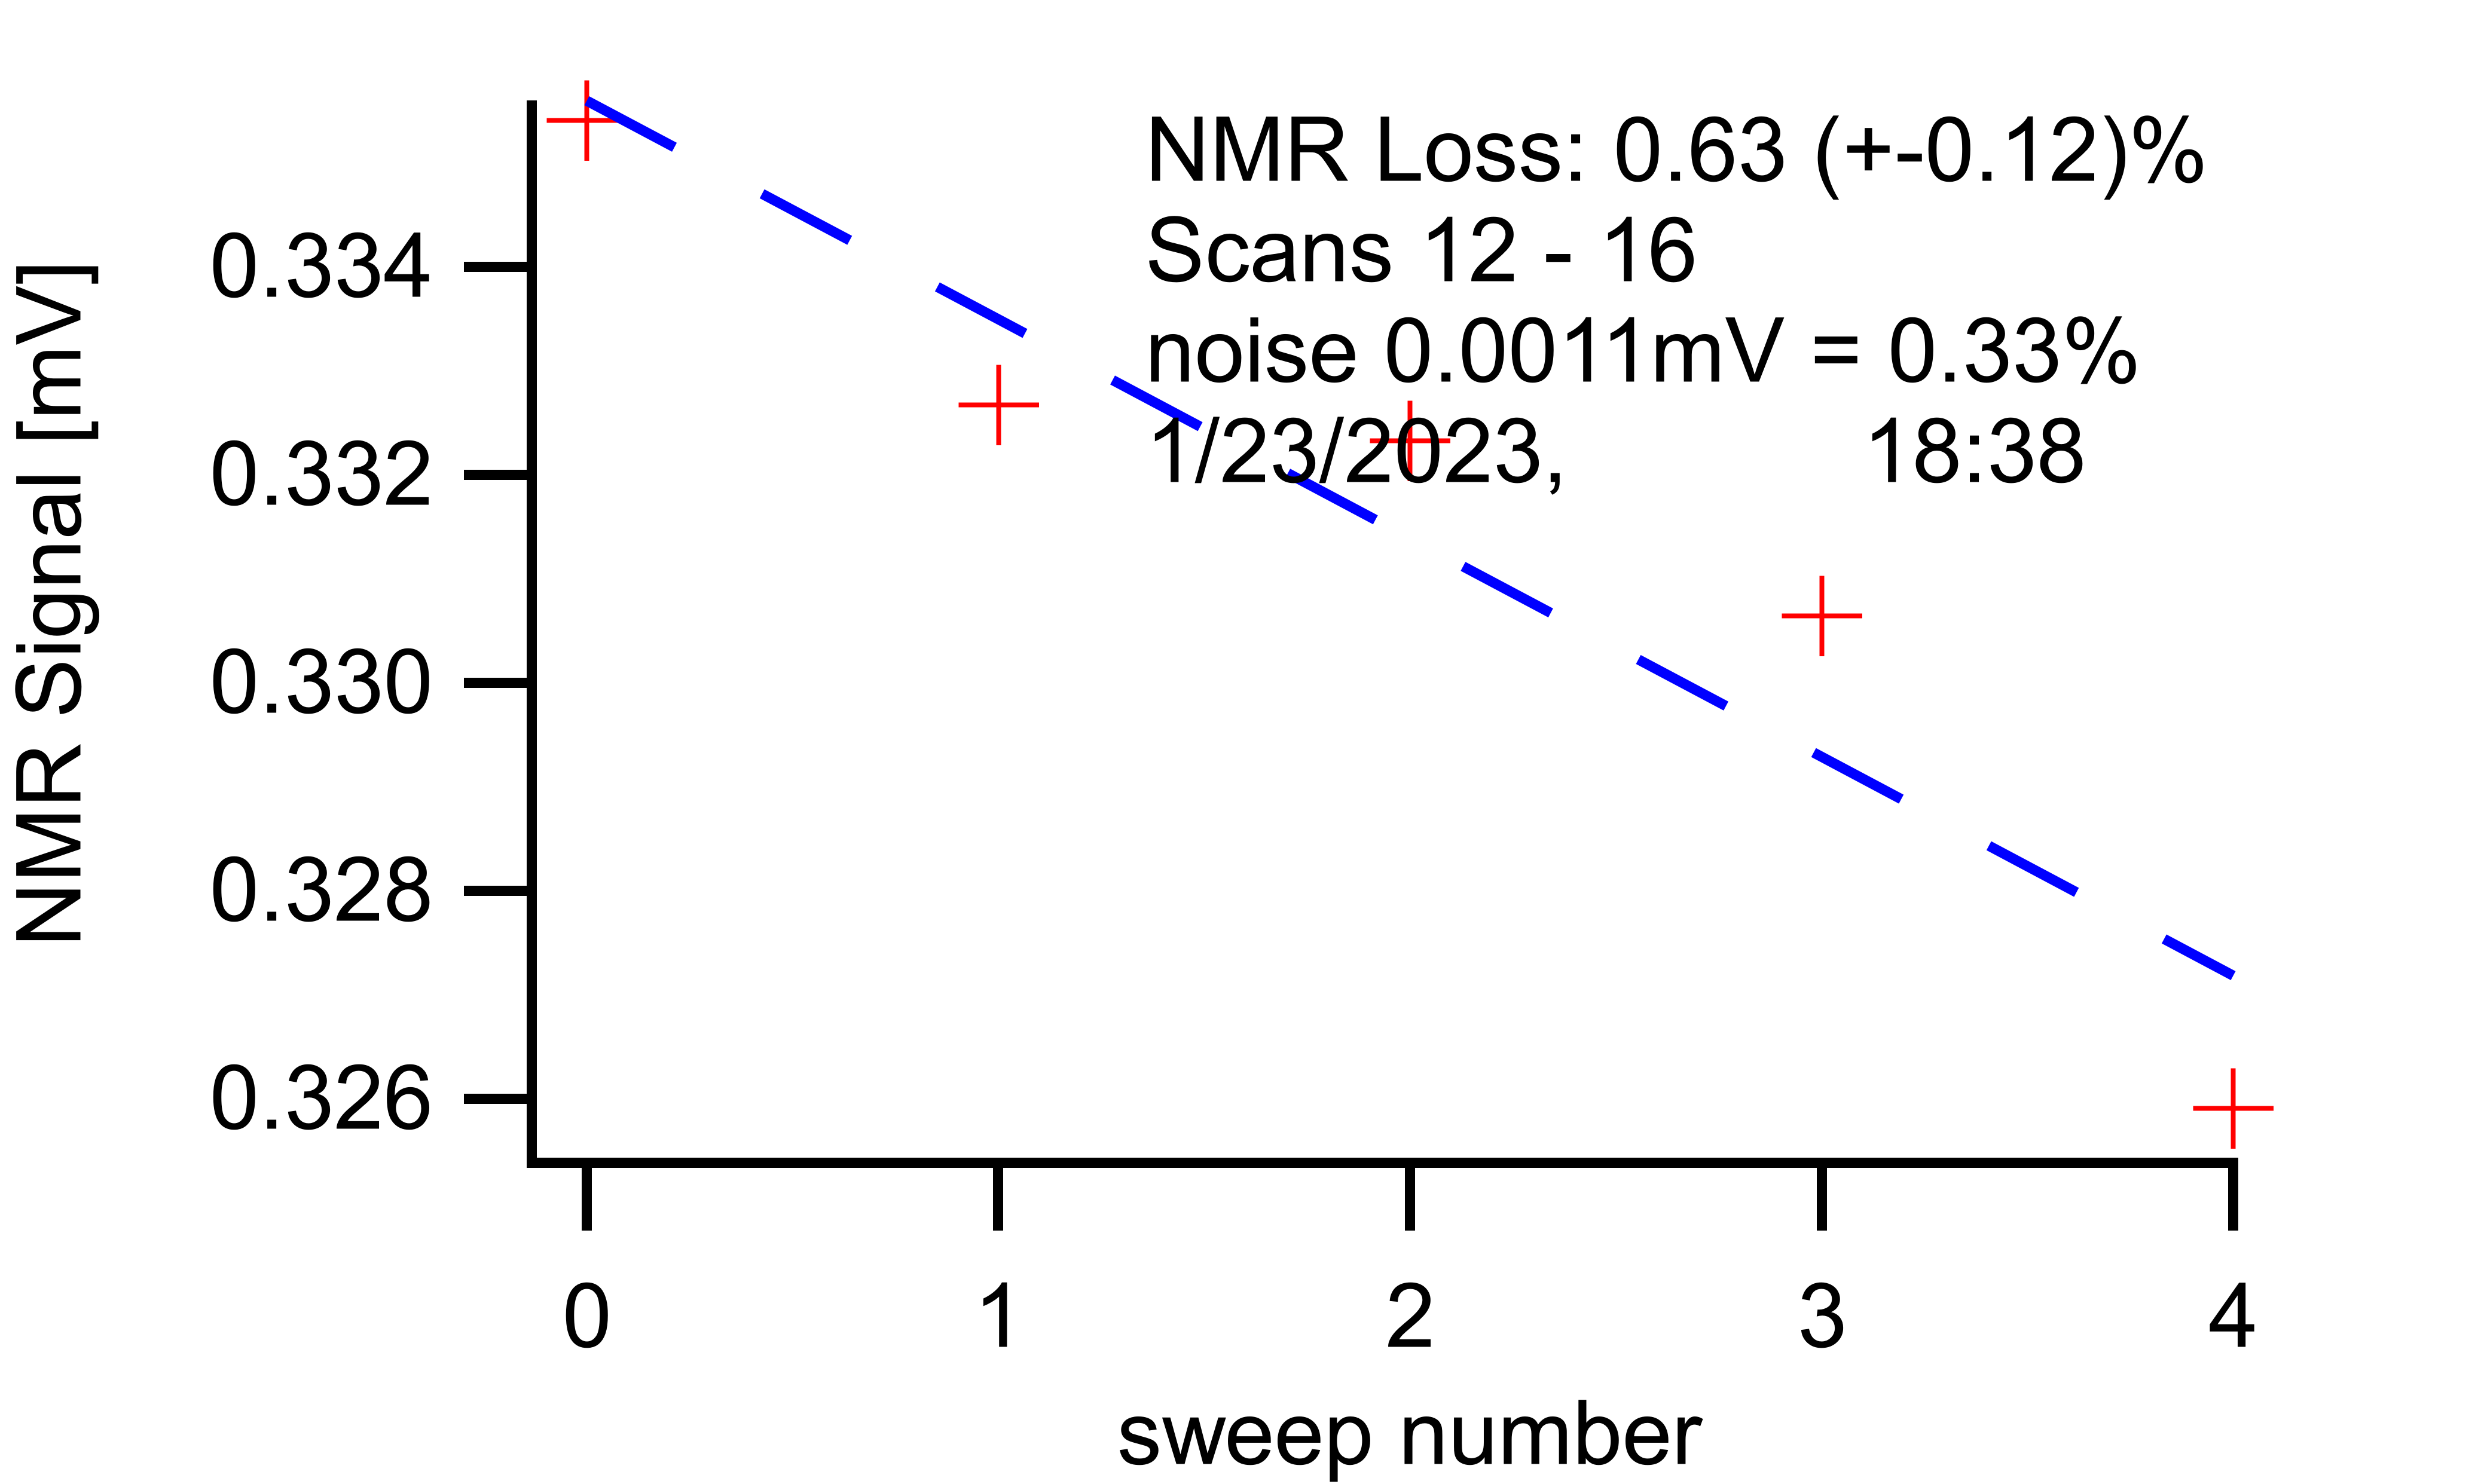
\includegraphics[width=\textwidth]{figures/chapter3-figs/NMRLoss_graph.png}
    \caption{Measured loss in FID response signal after 5 consecutive FID measurements. FID response is in red and the fit is the blue curve. }
    \label{fig:NMRLoss}
\end{figure}
\clearpage}

\afterpage{
\begin{figure}
    \centering
    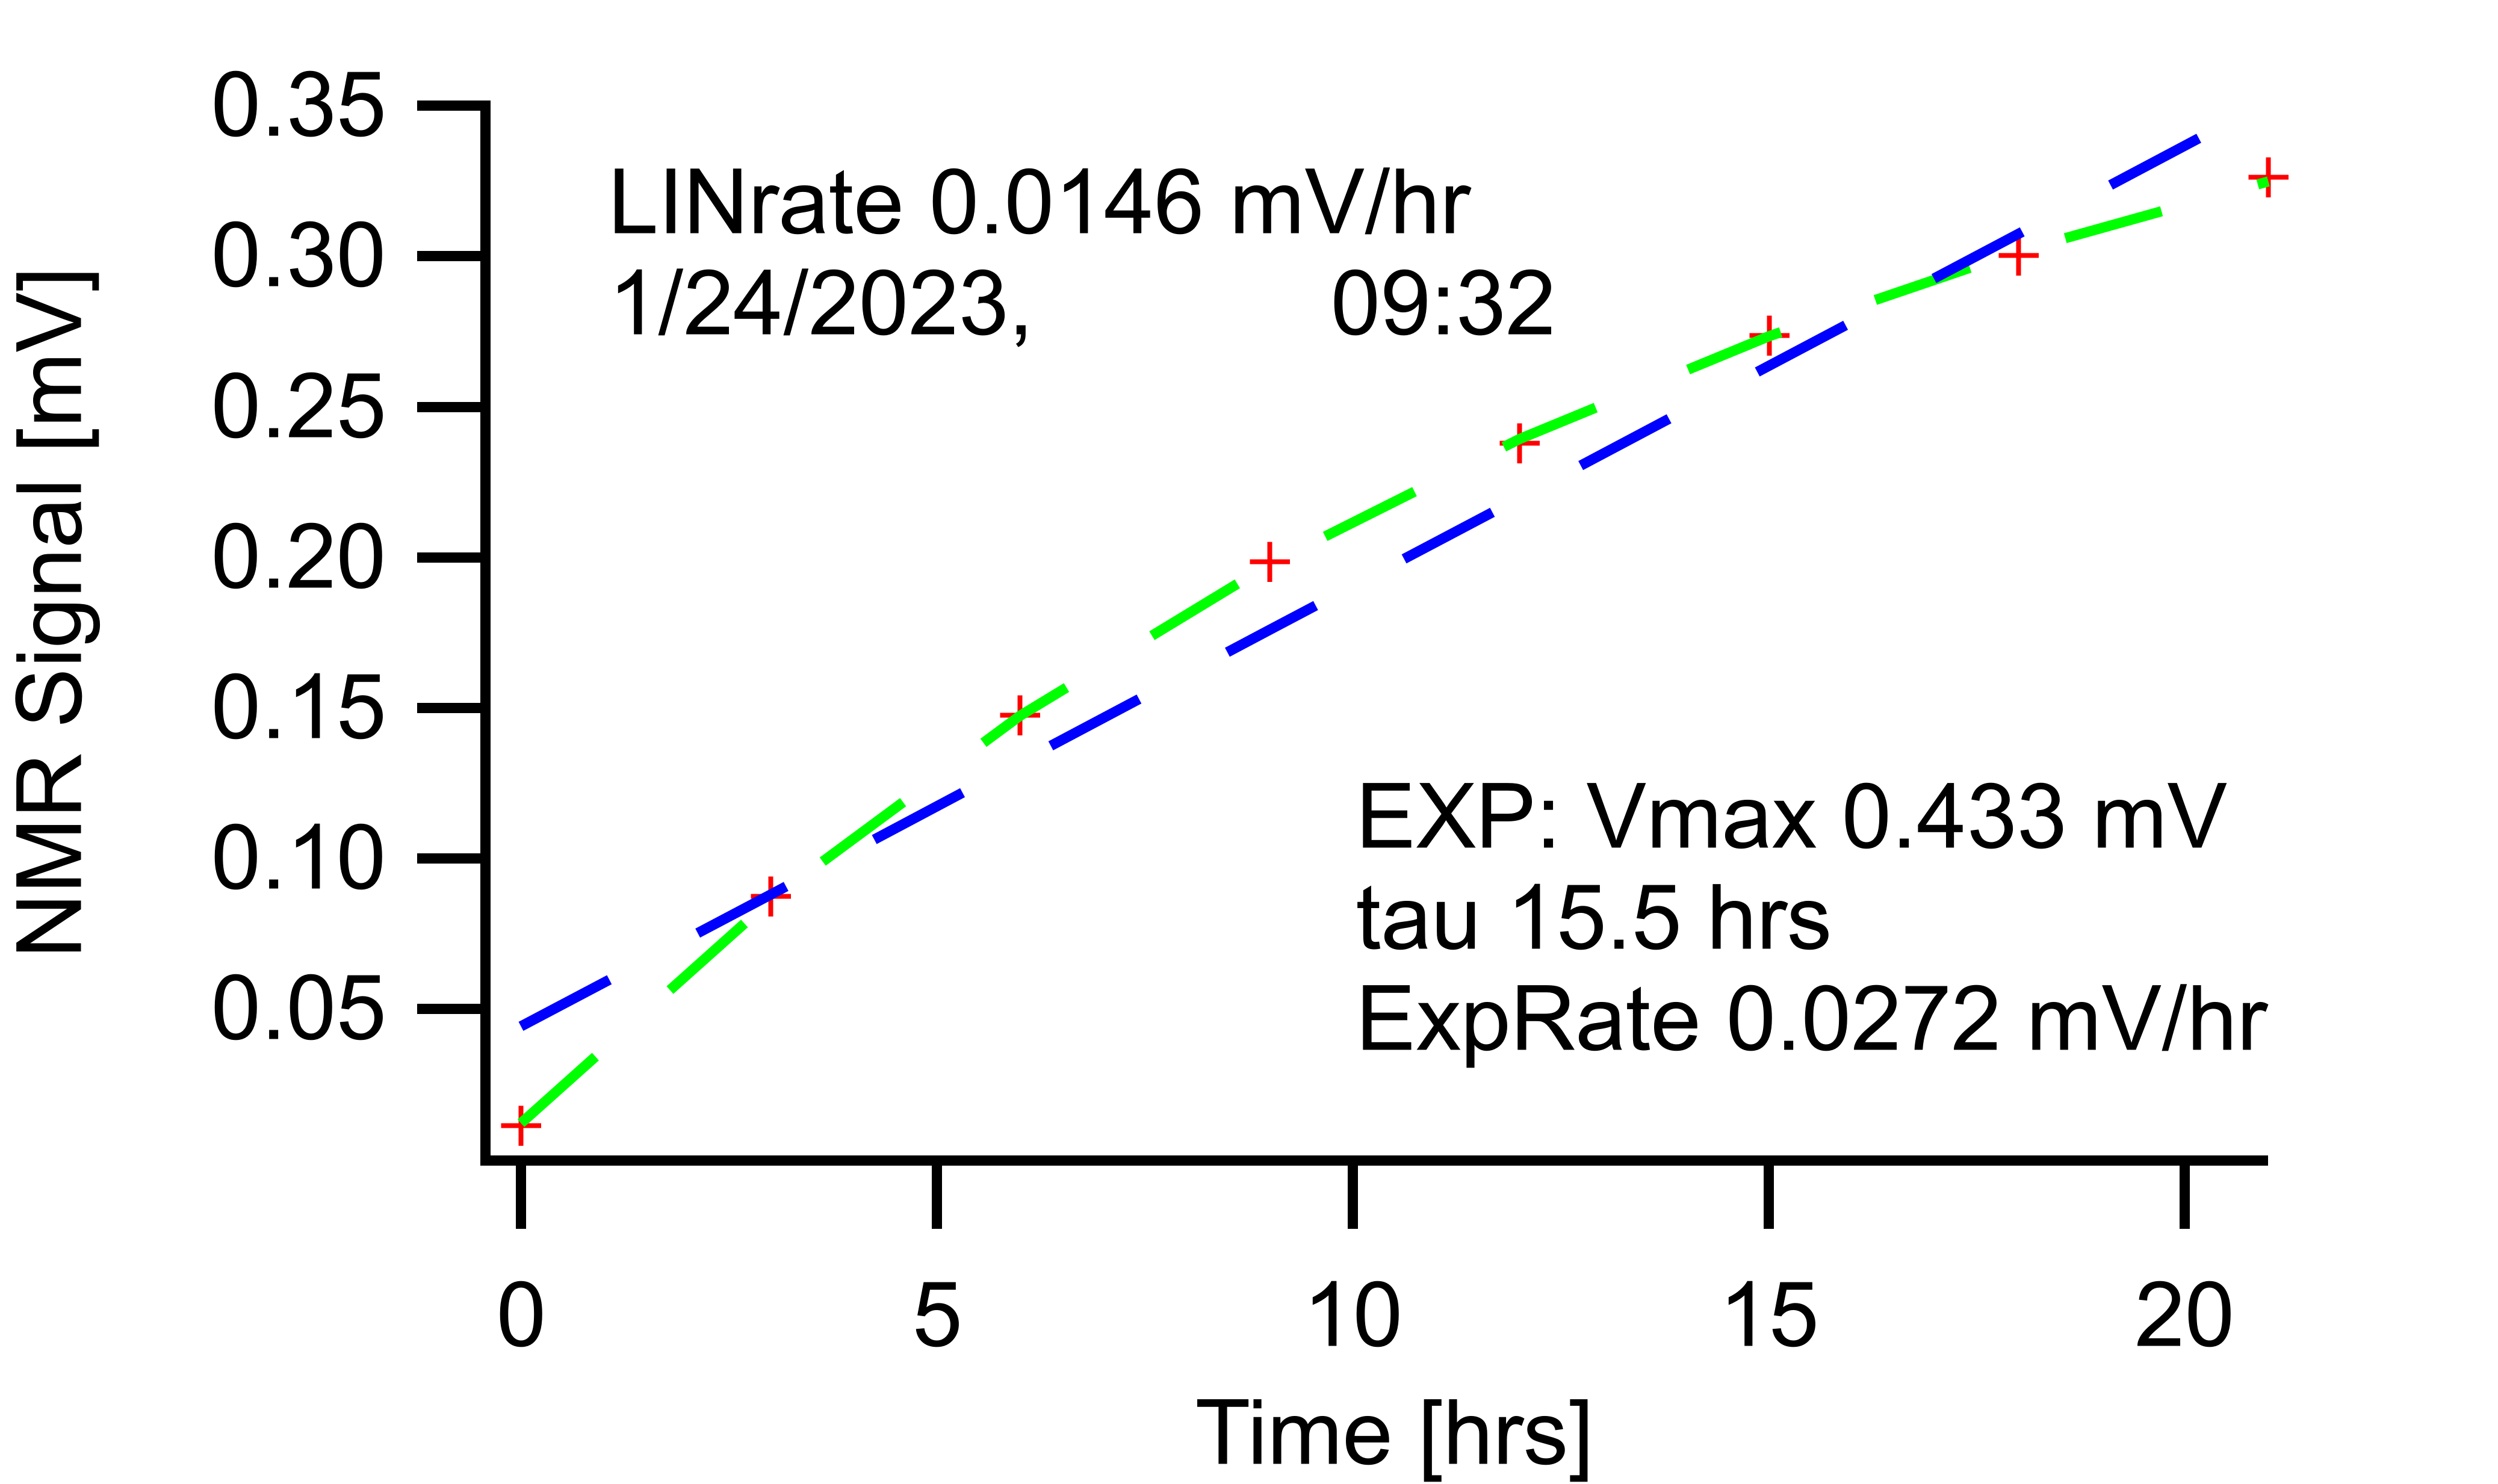
\includegraphics[width=\textwidth]{figures/chapter3-figs/Rate_graph.png}
    \caption{Response of the FID from the $^3$He over a course of time during the SEOP operation. The red points are the measured value and the green curve is the exponential growth fit.}
    \label{fig:spinup}
\end{figure}
\clearpage}

\afterpage{
\begin{figure}
    \centering
    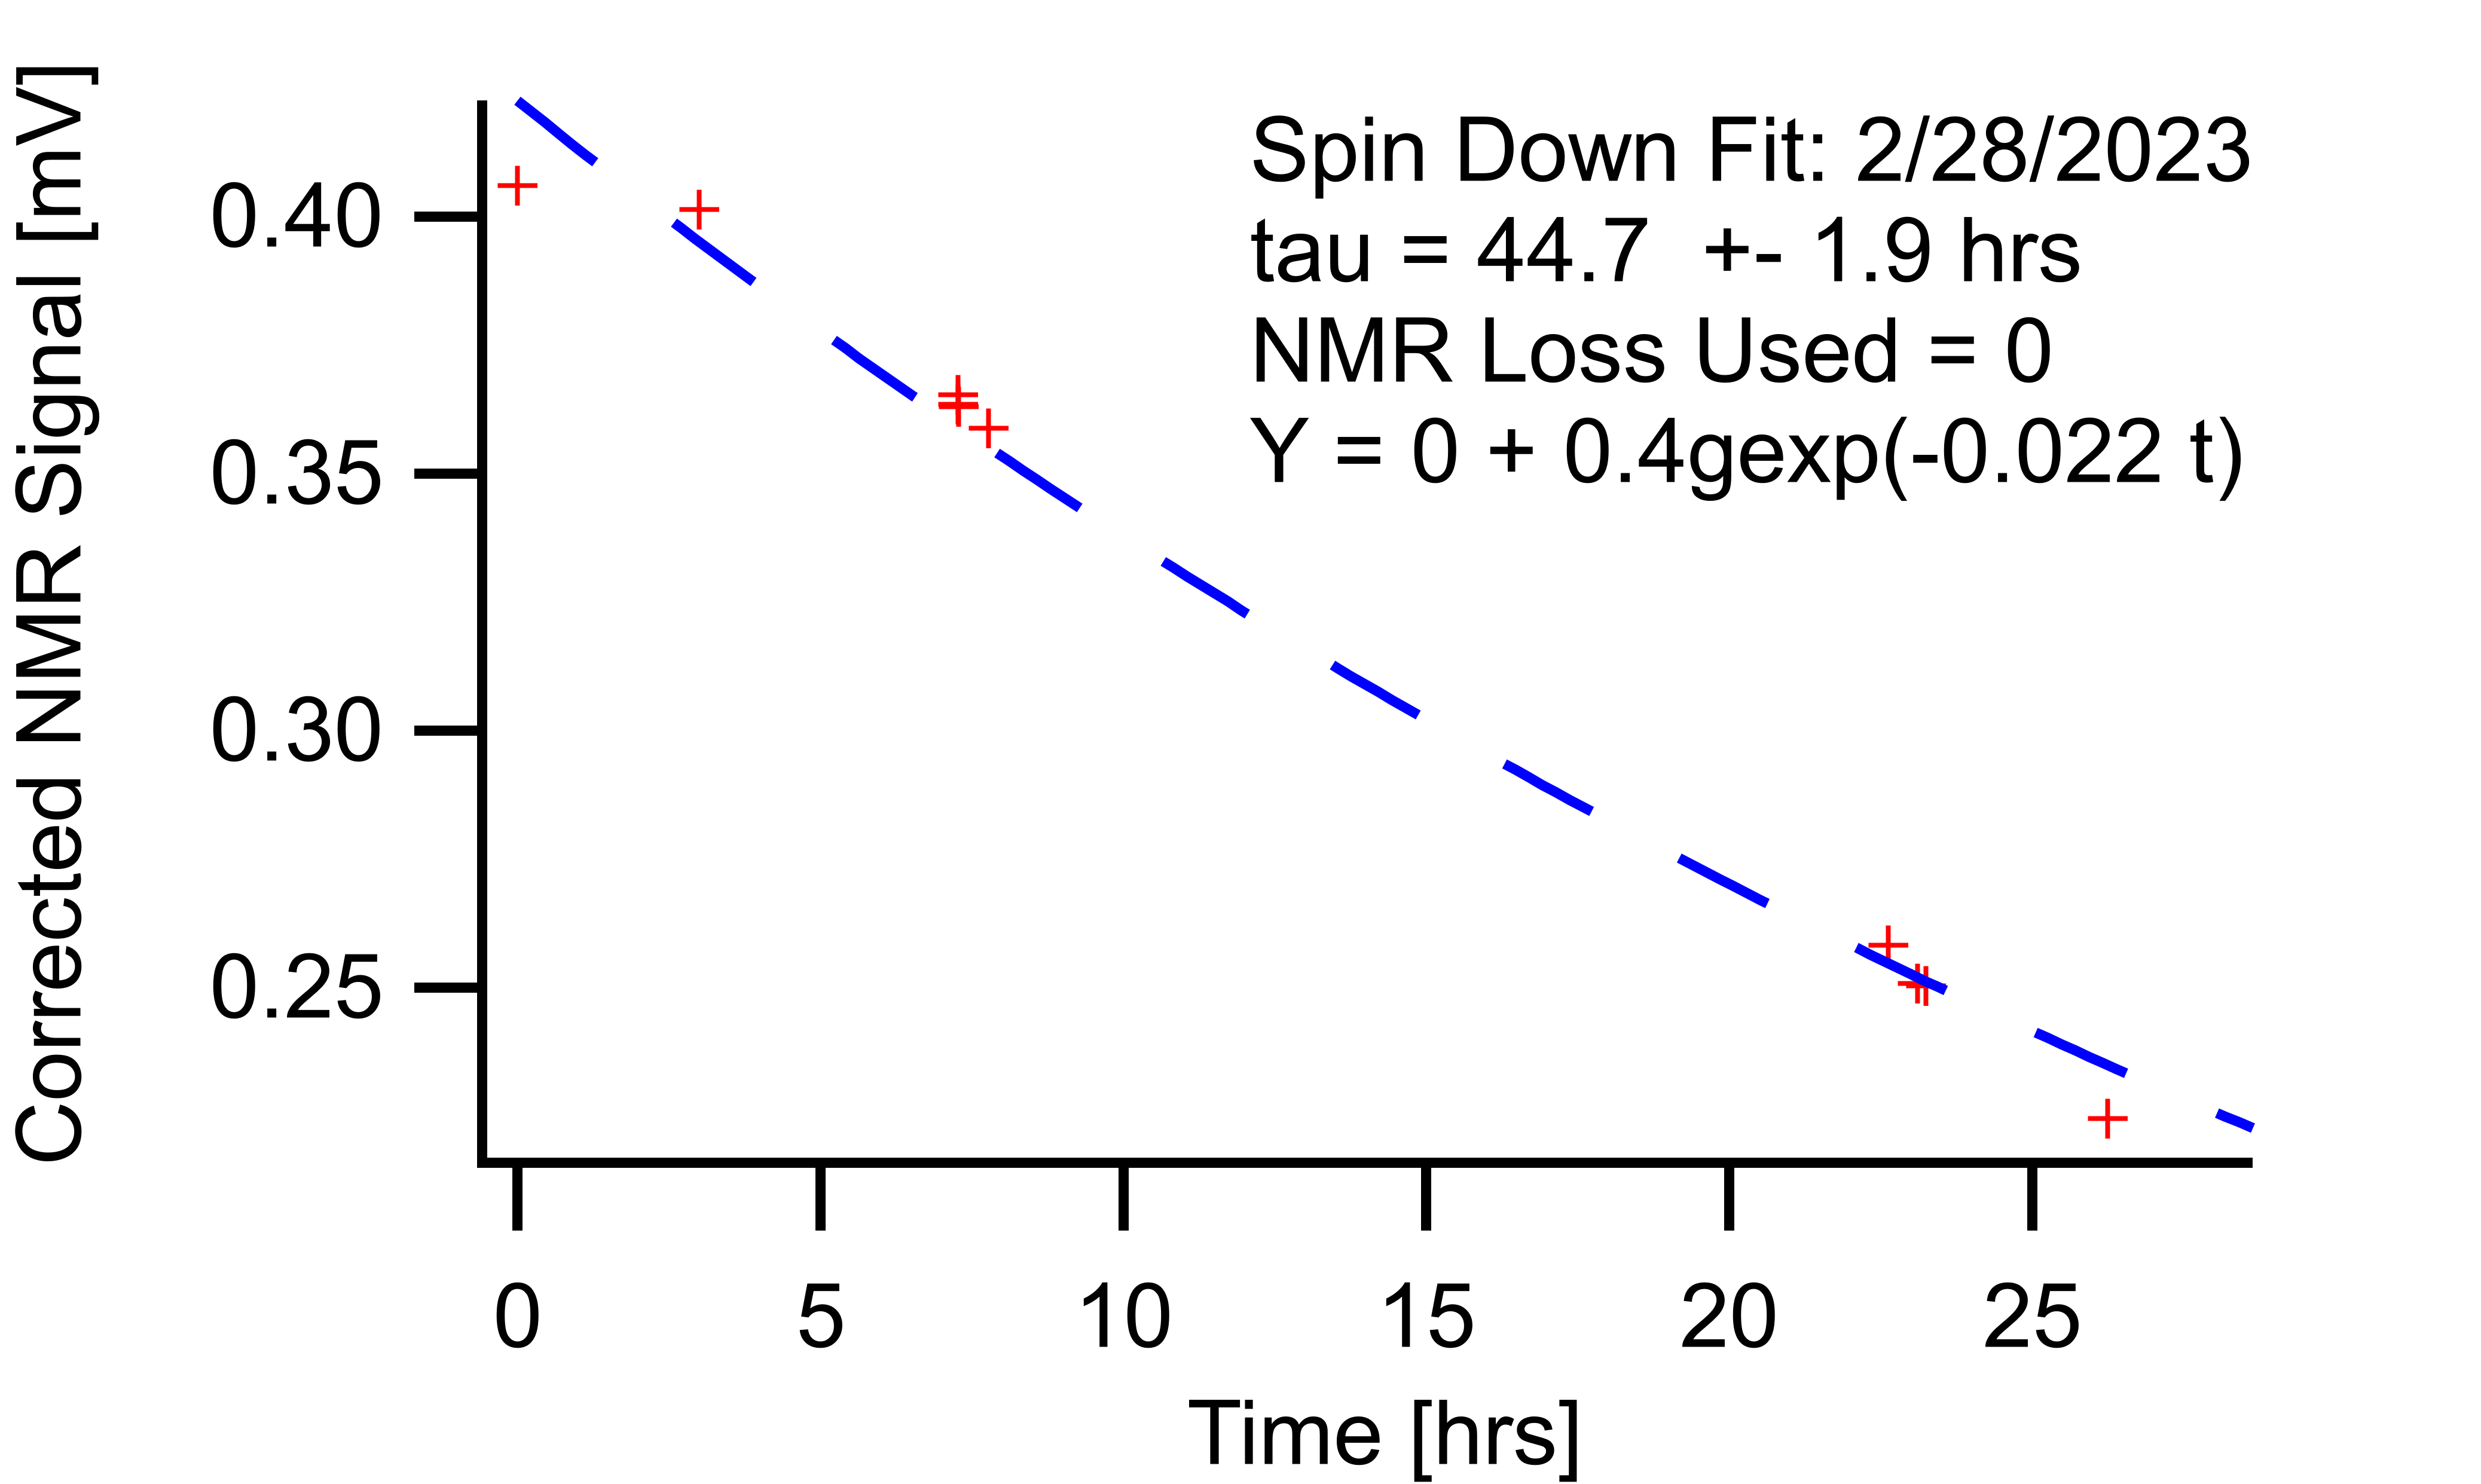
\includegraphics[width=\textwidth]{figures/chapter3-figs/spindown_phase2_2023feb30.png}
    \caption{Response of the FID from the $^3$He over a course of time after the SEOP operation is turned off. The red points are the measured value and the blue curve is the exponential decay fit.}
    \label{fig:spindown}
\end{figure}
\clearpage}

\subsubsection{Adiabatic Fast Passage}

In AFP NMR, an RF magnetic field, applied transverse to the static holding magnetic field of the $^3$He cell, is swept such that it passes through the Larmor frequency of the precessing $^3$He spins in the static magnetic field. Once the RF field sweeps beyond the resonance, the $^3$He polarization is inverted \cite{Abragam1961, Slichter1996}. The RF frequency's frequency sweep and amplitude are optimized to ensure a robust polarization inversion. 

%If a pickup coil transverse to both the static and rf magnetic fields is employed, a signal proportional to the magnetization is obtained. In order to minimize the large background from inadvertent pickup of the applied rf field, the pickup coil must be carefully adjusted to be orthogonal to the driving rf magnetic field. An absolute $^3$He polarization measurement can be obtained if the response of the pickup coil and associated electronics is calibrated using a thermally polarized water cell with exactly the same size and geometry as the $^3$He cell. Despite the extremely small thermal polarization of the order of 10-8 in typical holding fields of a few mT, these calibrations can be performed with uncertainties of a few percent. [In principle the magnitude of the AFP signal could be determined absolutely for a given apparatus, but in a study of this approach discrepancies of between 20\% and 50\% were observed with cell to cell variations (Chen et al., 2011).] Further descriptions of this technique and its application to electron-scattering targets (Chupp et al., 1987; Romalis et al., 1998), polarimetry of low-pressure MEOP cells (Lorenzon et al., 1993), and polarized gas MRI11 have been reported. 

%Whereas losses of a few tenths of a percent are typically encountered for AFP, techniques have been developed to substantially reduce these losses. The primary motivation has been for neutron spin-filter cells that are not actively optically pumped on the beam line, but in which the $^3$He polarization may be frequently inverted during use so as to invert the neutron polarization. Besides the usual optimization of rf magnetic-field strength and sweep rate, the rf field is modulated by a Gaussian envelope during the sweep (Petoukhov et al., 2006; McKetterick et al., 2011). Using this approach,losses of 10-5 per flip have been obtained. In a compact rf solenoid with shielding to confine the rf field, loss as low as 0.03\% was reported (Ye et al., 2013).

The primary usage of the AFP technique has been to invert the polarization of $^3$He cells, to analyze polarized neutron beams or characterize the efficiencies of guide field or spin flipper components in neutron beam experiments. RF frequency techniques have been developed to to perform AFP with high efficiencies. This section describes the AFP setup of the in situ system and the performance results on the polarized $^3$He cell, Soccer. The digitally generated voltage waveform used to provide the frequency sweep as well as a coil pair used to create the RF magnetic field are described. 

A sinusoidal waveform was used to create the required RF magnetic field. The linear frequency spread, $\omega(t)$, was set to sweep through the $^3$He resonance frequency from a range of $\omega_1$ and $\omega_2$, lasting a duration of $t_p$ in secs.
\begin{equation}
    \omega(t) = \frac{\left \lvert \omega_2 - \omega_1  \right \rvert}{2t_p} t + \omega_1 
\end{equation}
In order to ensure an adiabatic transition during the sweep, the amplitude of the sinusoidal wave is modulated with a Gaussian envelope for a rising and falling edge.
\begin{equation}
    B_{RF}(t) \propto \exp\left(   -\frac{[\omega(t) - \omega_L]^2}{\sigma^2}    \right) sin(\omega(t) \cdot t)
    \label{eq:AFPrf}
\end{equation} 
where $\omega_L$ is the $^3$He Larmor frequency and $\sigma$ parametrizes the frequency sweep width of the envelope \cite{Parnell2011}. \Cref{eq:AFPrf} is associated with any generic AFP frequency sweep and was tuned and optimized to work for the AFP requirements of this experiment. 

Previous AFP studies of $^3$He cells in \cite{Petoukhov2006, McKetterick2011} have shown that the maximum amplitude of the envelope should be no more than 10\% of the magnitude of the holding magnetic field, $B_0$. \cite{Petoukhov2006, McKetterick2011} have also shown that for a coil pair that produced a RF field over the required frequency range, $\Delta \omega = \omega_2 - \omega_1$, a Gaussian sweep with a FWHM of 10\% of $\Delta \omega$ created the most efficient spin flips. This amplitude modulated frequency sweep will invert the $^3$He polarization, regardless of the RF field's homogeneity, since it eliminates any high frequency noise in the the AFP pulse \cite{Garwood2001}.

$\Delta \omega$ of the sweep depends on the variation in the the holding magnetic field magnitude. This means that the frequency sweep has to encompass a broad range of the $^3$He resonant frequencies arising from any longitudinal variation in $B_0$ across the $^3$He cell. $\Delta \omega$ can be widened to ensure that the AFP sweep has a small amplitude at the start and at finish of the sweep for the off resonance $^3$He frequencies and at the same time, a large amplitude for the $^3$He resonant frequencies to perform a robust spin flip. Testing in \cite{McKetterick2011} have shown that a frequency range, $\Delta \omega$ of $\frac{\omega_L}{2}$ to $\frac{3\omega_L}{2}$, delivered the most efficient spin flips.

The in situ system has a built in rectangular coil pair used to provide the AFP RF field. The coils made of 18AWG (diameter = 0.0428 inches) copper wire and consist of 15 turns/coil. The total resistance of the coil pair is 0.5$\Omega$ and an inductance of 0.317 mH. The Q-factor as $\frac{\omega_L L}{R}$, where $L$ is the inductance and $R$ is the resistance, comes out to be 68, indicating the the RF coil pair is operating in the inductive regime with minimal power loss to impedance. This setup is shown in \cref{fig:NMRsetup}. The $^3$He has a reuced gyromagnetic ratio of 3.24 kHz/G, therefore, the resonant frequency for the 12.7 G holding magnetic field created by the Merritt coil is 41.16 kHz. These frequencies were created  with the same digital I/O card as used in the FID NMR. Using the IgorPRO programming package, a digital waveform generator, was used to to generate the AFP sweep waveform based on the parameters of desired AFP sweep. A frequency binning of 1 microhertz was used to avoid aliasing. This fine binning was possible because of the sampling rate of the digital I/O card used. The I/O card converts the digital AFP waveform to an analog waveform, which is sent to the AFP coil pair via a power amplifier set to a 50$\times$ gain. This setup is illustrated in \cref{fig:NMRsetup}. The parameters shown in \cref{tab:AFP_params} were used to generate an AFP pulse, shown in \cref{fig:AFPtime}, from the DAQ board as:
\begin{equation}
 \begin{aligned}
    F_{AFP}(t_i)  = V_{RF} & \times \exp\left( -\frac{ \left[\left(f_{min}-R_{sweep} \times t_i \right)- f_{cent} \right]^2 }{f_{FWHM}^2}    \right) \\
    & \times sin \left(2 \pi \left(f_{min} + \frac{1}{2} R_{sweep} \times t_i \right) \times t_i \right)
\end{aligned}   
\end{equation}
where
\begin{equation}
    t_i = \cfrac{f_{max}-f_{min}}{\cfrac{R_{sweep}}{t_{step}}}
\end{equation}
and the total time of the AFP pulse duration comes out to be:
\begin{equation}
    t_{total} = \frac{f_{max}-f_{min}}{R_{sweep}}
\end{equation}

\afterpage{
\begin{table}
\centering
\caption{List of parameters used for AFP NMR to invert the polarized $^3$He.}
\label{tab:AFP_params}
\begin{tabular}{@{}lc@{}}
\toprule
AFP Parameters               & AFP Parameter Values \\ \midrule
Center Frequency {[}Hz{]}    & 41160                \\
Frequency Sweep Rate {[}kHz/sec{]}           & 50-200               \\ 
Freq. FWHM {[}Hz{]}          & 7000               \\
Minimum Frequency {[}Hz{]}           & 0.6 $\times$ 41160                     \\
Maximum Frequency {[}Hz{]}          & 1.5 $\times$ 41160                  \\
Amplitude {[}V{]}            & 2.0               \\
A0 timestep {[}sec{]}           & $1\times10^{-6}$       \\ 
\bottomrule
\end{tabular}
\end{table}
\clearpage}

\afterpage{
\begin{figure}
    \centering
    \includegraphics[width=\textwidth]{figures/chapter3-figs/AFP_waveintime.png}
    \caption{Modulated RF pulse used for AFP based on the parameters in \cref{tab:AFP_params}.}
    \label{fig:AFPtime}
\end{figure}
\clearpage}

There are two indicators that determine the performance of an AFP flip. The first is to determine whether the AFP has reversed the polarization of the $^3$He nuclei and the second is to measure the relative loss in $^3$He polarization after an AFP spin flip sequence \cite{McKetterick2011, Parnell2008}. The FID NMR described in the previous section was used to characterize the performance of the AFP flip sequence. The change of phase of the FID signal determines the relative polarization state of the $^3$He analyzer cell. The polarized $^3$He FID signal and spin inverted $^3$He FID signal should show a difference in phase angle of $180 \degree $ indicating that a change in $^3$He polarization has taken place \cite{Parnell2008, Parnell2011}. The FID response measured from Soccer, before and after AFP pulse was deployed, is shown \cref{fig:AFPflip}. The before and after FID responses show a $180 \degree $ change in phase, indicating a successful inversion of $^3$He polarization from an AFP pulse.

%The initial amplitude of the FID is found by fitting the data to the equation :
%%    f(t) = \frac{1}{2} V_{pp} sin(\omega_L t + \phi) \exp\left( \frac{-t}{T_2^*}    \right)
%    \label{eq:FID}
%\end{equation}
%where $V_{pp}$ is the peak to peak voltage caused by the spin precession tipping from the FID pulse and $\omega_L$ is the Larmor frequency and $\phi$ is the phase of the sinusoidal wave. The exponential decay envelope of the FID response has a transverse relaxation time constant, $T_2^*$, which is dependent upon the inhomogeneities in the holding field, $B_0$. The decay in FID amplitude was plotted against time and fitted to the \cref{eq:FID}, to extract the max amplitude, frequency, phase and $T_2^*$. 

%\Cref{fig:AFPflip} shows that although the two $^3$He polarization states should be experiencing the same magnetic field and the same gradients, the observed FID signals for the unflipped and flipped states have slightly different $T_2^*$ time. This can be attributed to radiation damping effects \cite{Augustine2002} and the onset of masing in the high energy state \cite{Chupp1994}. There may also be contributions to the local magnetic field due to the reversal of the bulk $^3$He polarization. 

The relative loss in $^3$He polarization arising from performing AFP NMR was measured by recording FID signals before and after performing 10 consecutive AFP sweeps. The initial tests showed losses of 0.053\% loss in $^3$He polarization per flip. This loss is minimal and adequate for the in situ system.

When AFP is performed, the $^3$He polarization becomes flipped with respect to the holding magnetic field. This means that the D1 transition is now from $m_s=-1/2$ and the circularly polarized light, $\sigma_+$ is no longer useful. As a matter of fact it will depolarize the alkali and hence, the $^3$He. Therefore, the LCR was adjusted to provide $\sigma_-$ D1 circular polarized light every time $^3$He polarization was flipped with respect to $^3$He and vice versa.

\afterpage{
\begin{figure}
     \centering

     \begin{subfigure}{0.9\textwidth}
         \centering
         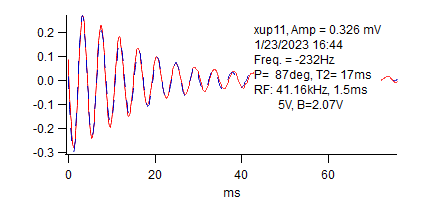
\includegraphics[width=0.9\textwidth]{figures/chapter3-figs/xup_graph.png}
         \caption{FID response prior to an AFP pulse.}
         \label{fig:FIDpriorAFP}
     \end{subfigure}
     \hfill
     \begin{subfigure}{0.9\textwidth}
         \centering
         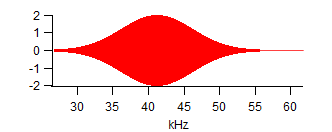
\includegraphics[width=0.75\textwidth]{figures/chapter3-figs//AFPF_RF.png}
         \caption{AFP Pulse used to invert $^3$He polarization.}
         \label{fig:AFPpulsefreq}
     \end{subfigure}
     \hfill
     \begin{subfigure}{0.9\textwidth}
         \centering
         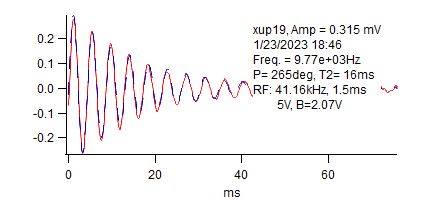
\includegraphics[width=0.9\textwidth]{figures/chapter3-figs/xup_graph_postafp.png}
         \caption{FID response post an AFP pulse.}
         \label{fig:FIDpostAFP}
     \end{subfigure}
        
        \caption{Inversion of $^3$He polarization in Soccer. Notice the 180$\degree$ phase change from (a) to (c) after the AFP pulse (b) is applied. Red curve is the measured response and the blue curve is the fit.}
        \label{fig:AFPflip}

\end{figure}
\clearpage}

\subsection{Electron Paramagnetic Resonance Spectroscopy}

Electron Paramagnetic Resonance Spectroscopy is used as an additional diagnostic to characterize the $^3$He polarization. EPR spectra is obtained by detecting the fluorescence from a polarized $^3$He cell under the application of transverse RF magnetic field, which slightly changes the alkali polarization by sweeping through the alkali Zeeman resonances \cite{Romalis1998, Chann2002a, Kramer2007}. The polarized alkali serve as insitu comagnetometers of the classical dipole magnetization produced by the polarized $^3$He. The field experienced by the polarized alkali from the polarized $^3$He is \cite{Romalis1998, Schaefer1989, Barton1994}:
\begin{equation}
    B_{He} = \mu_{He} \kappa_{eff} [He] P_{He}
\end{equation}
where $\mu_{He}$is the $^3$He magnetic moment, and $\kappa_{eff}$ is defined as:
\begin{equation}
    \kappa_{eff} = \kappa_0 + \frac{3}{8\pi}C-1
\end{equation}
where $\kappa_0$ is a dimensionless proportionality factor \cite{Romalis1998} and $C$ is the constant for a cylindrical $^3$He cell \cite{Chann2002} with radius, $r$, and length, $l$, like Soccer as:
\begin{equation}
    C = \frac{8\pi}{3} \left( \frac{3}{2} \left( \sqrt{1 + \frac{r}{l}^2} - \frac{r}{l} \right)  \right)  
\end{equation}

The field $B_{He}$ produces an EPR frequency shift \cite{Romalis1998}:
\begin{equation}
\label{eq:EPRshift}
    \Delta \nu_{EPR} = \gamma_A B_{He} = \frac{\gamma_e}{2 I_A + 1} B_{He}
\end{equation}
where $\gamma_e =$28 GHz/T is the electron's gyromagnetic ratio. This means that $^3$He can be extracted via the EPR frequency shift. $\kappa_0$ has been measured for alkali atoms and is shown in \cref{tab:spinexrate} \cite{Gentile2017}. 

Since the alkali are also highly polarized and undergoing spin exchange with $^3$He, the EPR spectrum becomes proportional to the square of the RF magnetic field \cite{Romalis1998}. For small holding magnetic fields, this leads to a splitting between EPR levels arising from the second-order Zeeman effect in B \cite{Gentile2017} as: 
\begin{align}
    x \frac{\gamma_e^2}{\Delta E_{hf}} B^2
\end{align}
where $\Delta E_{hf}$ is the hyperfine splitting and 
\begin{align}
x = \frac{4(2m-1)}{(2I_A+1)^2} =
    \begin{cases}
        \frac{2}{9} & \text{for $^{85}$Rb with I$_A$ = 5/2}\\
        \frac{1}{2} & \text{for $^{87}$Rb and K with I$_A$ = 3/2} 
    \end{cases}
\end{align}

In SEOP, the the hyperfine levels at play during EPR are m=$F_{max}$ $\rightarrow$ $F_{max}-1$ and $F_{max}-1$ $\rightarrow$ $F_{max}-2$, where $F_{max} = I_A+1/2$ is the maximum angular momentum state of the alkali under D1 transition of alkali \cite{Romalis1998, Gentile2017}. The F$_{max}$ line is unperturbed, while the $F_{max}-1$ line is broadened from the spin exchange \cite{Appelt1999}. As mentioned earlier, even though the alkali excited to the P state are mostly quenched by N$_2$, a small fraction of them still decay by fluorescence. Thus, if the RF magnetic field tuned at the alkali resonance frequency induces a transition from F$_{max}$, m=$F_{max}$ to F$_{max}$, m = $F_{max}-1$, then the number of the alkali atoms in m = $F_{max}-1$, which can absorb light will be increased and hence, the fluorescence will increase \cite{Romalis1998, Gentile2017}. In practice, the D1 light of the laser dominates the D1 fluorescence emission of the $^3$He cell. Therefore, alkali's D2 transition emission is used to measure the EPR frequency shift as a function of RF frequency sweep. Since the EPR shift depends on the $^3$He magnetization, AFP flip on $^3$He polarization with respect to the magnetic field is performed to isolate the EPR frequency shift from other effects \cite{Romalis1998}. This gives double the EPR frequency shift due to the AFP flip.

%There are two ways to measure the EPR frequency shift: the Amplitude Modulation (AM) measurement and the Frequency Modulation (FM) measurement. The AM method measures the intensity of the D2 emission with respect to the RF frequency while the FM method measures the derivative of the intensity with respect to the frequency.

The setup used for the EPR for the in situ $^3$He system is shown in \cref{fig:NMRsetup}. A function generator programmed digitally was used to create the modulated RF field. The RF field was applied to the $^3$He cell by a circular coil, about the size of the $^3$He cell, mounted on one side of the $^3$He cell. The fluorescence from the $^3$He cell was measured using a photodiode with a D2 filter placed along the exposed face of the $^3$He cell. The signal from the photodiode was sent to the lock-in amplifier, as mentioned in the previous section, and referenced to the modulation frequency of the function generator. By scanning the RF frequency, the change in the measured photodiode intensity as a function of frequency was recorded. When the RF frequency sweeps through the EPR resonance frequency, the measured signal should reach the maximum and therefore, the EPR frequency can be extracted.

Unfortunately, after performing many sweeps and trying several parameters, a photodiode signal was not observed. Possible causes for this could be the presence of gradeints in the holding magnetic field, which can change the $^3$He magnetization, change in cell temperature as the $\kappa_0$ has slight temperature dependence and can change $ \Delta \nu_{EPR}$ by 0.14\%/$\degree$C, or the the $^3$He density of the cell Soccer is too low to extract an EPR response. Further diagnosis of this problem need to be performed.


\subsection{Neutron Transmission}

There is a large neutron absorption cross section for $^3$He, which arises from a broad($\Gamma$=400 keV) , unbound, resonance ($J^{\pi}=0^{+}$) located 650 keV below the neutron binding energy of the $^4$He$^{*}$ intermediate state, that yields a proton and a triton \cite{Csoto1997}. The reaction can be shown as:
\begin{equation}
    n+ {^3He} \rightarrow {^4He^*} \rightarrow t + p
\end{equation}
Furthermore, the ground state of $^3$He wavefunction is dominated by the singlet state, in which the spins of the two protons negate due to the exclusion principle, and the $^3$He nuclear spin is effectively given by the unpaired neutron \cite{Bissey2002, Friar1990}. This leads to a strong spin dependence in the absorption cross section; 5333 barns for 25 meV neutron capture on $^3$He with antiparallel spins and nearly zero for parallel spins \cite{Passell1966}. The ratio of absorption cross section to the total reaction cross sections for this reaction has been found to be near unity with an error of less than a percent, indicating that absorption mechanism dominates the reaction \cite{Huber2014} and non-resonant scattering cross section is small, measured to be 6 barns \cite{Mughabghab1981} \footnote{The neutron and $^{3}He$ capture can also undergo another reaction branch, $n+ {^3He} \rightarrow {^4He} + \gamma$, but the cross section for this branch is in microbarns \cite{Zurmuhle1963}.}. 

Hence for an ideal 100\% polarized $^3$He cell, neutrons with spins antiparallel to $^3$He polarization will get captured, while neutrons with spins parallel to $^3$He polarization will transmit through the NSF. The resulting transmitted neutrons from the NSF will be 50\% of the initial intensity and 100\% polarized, with respect to the guide magnetic field. Subsequently, imperfect $^3$He polarization will be inefficient in discriminating the neutron polarization as well as decrease the neutron transmission. The efficacy of the NSF can be changed by picking the cell thickness, i.e. the neutron opacity, based on the needs of the experiment. In addition to being spin dependent, the n-$^3$He absorption cross section, is inversely proportional to the neutron wavelength as $\sigma_0/\lambda_0$ in units of 10$^{-24}$ cm$^2$, hence longer wavelength (lower kinetic energy) neutrons require lesser opacities. For NSFs, opacity is adjusted by varying the pressure, $P$, in bars of $^3$He (i.e. the $^3$He number density, $n_{He}$, in units of cm$^{-3}$) and the length, $l$, in cm of the cell for a given neutron wavelength, $\lambda$, in \AA. The opacity, $\zeta$, can be written as:
\begin{equation}
    \zeta = -n_{He}l\frac{\sigma_0}{\lambda_0}\lambda(t) = 0.073 ~\text{bar$^{-1}$  cm$^{-1}$  \AA$^{-1}$} \cdot P \cdot l \cdot \lambda
    \label{eq:opacity}
\end{equation}
Hence, the transmission of an unpolarized monochromatic neutron beam through an unpolarized $^3$He cell can be determined from:
\begin{equation}
    T_{unpol} = T_e e^{-\zeta}
    \label{eq:Tunpol}
\end{equation}
where $T_e$ is the transmission through an empty glass cell, which for GE180 glass has been measured to be 88\% $\pm$ 2\% \cite{Chupp2007}.

The $^3$He polarization can be defined \footnote{Assuming no coherence between the two spin states.} as:
\begin{equation}
P_{He} = \frac{n_{He}^{\uparrow} - n_{He}^{\downarrow}}{n_{He}^{\uparrow} + n_{He}^{\downarrow}} =   \frac{n_{He}^{\uparrow} - n_{He}^{\downarrow}}{n_{He}}
\end{equation}
where $n_{He}^{\uparrow}$ is the number density of spin up particles and $n_{He}^{\downarrow}$ is the number density of spin down particles. The polarized $^3$He densities can be expressed in terms of $^3$He polarization as $n_{He}^{\uparrow} = \frac{n_{He}}{2}(1+P_{He})$ and  $n_{He}^{\downarrow}  = \frac{n_{He}}{2}(1-P_{He})$. If we now assume that $^3$He cell is polarized, then for an incident unpolarized neutrons, $N_0 = N_\uparrow + N_\downarrow$, the neutron intensity from the transmission for the two neutron spin states through the polarized $^3$He cell is given by:
\begin{equation}
    N_\uparrow = \frac{N_0 T_e}{2} e^{-\zeta} e^{\zeta P_{He}}
\end{equation}
and
\begin{equation}
   N_\downarrow = \frac{N_0 T_e}{2} e^{-\zeta} e^{-\zeta P_{He}}
\end{equation}
Now, with the neutron polarization defined \footnote{Again, assuming no coherence between the two spin states.} as:
\begin{equation}
    P_n = \frac{N_\uparrow - N_\downarrow}{N_\uparrow + N_\downarrow}
\end{equation}
the analyzing/polarizing, $P_n^{He}$, power of the $^3$He cell becomes
\begin{equation}
    P_n^{He} = \tanh{\left(\zeta P_{He}\right)}
    \label{eq:anal_power}
\end{equation}
and the transmission of the unpolarized beam through a polarized $^3$He cell becomes:
\begin{equation}
       T_{pol} = T_{unpol} \cosh{\left(\zeta P_{He}\right)}
       \label{eq:Tpol}
\end{equation}
Using the hyperbolic trigonometric identity, $1+\tanh^2{x} = \sech^2{x}$, $P_n^{He}$ can be expressed as:
\begin{equation}
    P_n^{He} = \sqrt{1 - \left(\frac{T_{unpol}}{T_{pol}} \right)^2}
    \label{eq:anal_power2}
\end{equation}
This implies that, $P_n^{^3He}$, can be accurately determined with only a relative neutron transmission measurements through a polarized $^3$He cell \cite{Greene1995, Coulter1990, Jones2000}. Because of the wavelength dependence, neutron transmission measurements can be performed with either monochromatic beams or with the time-of-flight (TOF) analysis for pulsed neutron beams.

For an incident neutron beam of 8.9~\AA\ and the Soccer cell parameters, the expected transmission and analyzing power analyzing of the cell soccer as a function of $^3$He polarization can be determined. This is shown in \cref{fig:soccer_exp}. The figure illustrates two important features of polarized $^3$He based neutron polarimetry. First, the higher the $^3$He polarization, the higher transmission of unpolarized neutrons from a polarized $^3$He cell is expected. Secondly, the higher the $^3$He polarization, the higher the analyzing power of the $^3$He cell (i.e. the $^3$He cell can discriminate between two neutron spin states more efficiently and provide a better spin contrast.)

\afterpage{ 
\begin{figure}
    \centering
    \includegraphics[width=\textwidth]{figures/chapter3-figs/SoccerLonestarcomparson.png}
    \caption{The analyzing power, $P_n^{^3He}$, and transmission, $\frac{T_{pol}}{T_{unpol}}$, as a function of $^3$He polarization for the cell Soccer with 0.8 bar pressure, 6.62 cm in length and an 8.9~\AA\ incident neutron beam.}
    \label{fig:soccer_exp}
\end{figure}
\clearpage}

\afterpage{
\begin{figure}
    \centering
    \begin{subfigure}[b]{0.75\linewidth}
        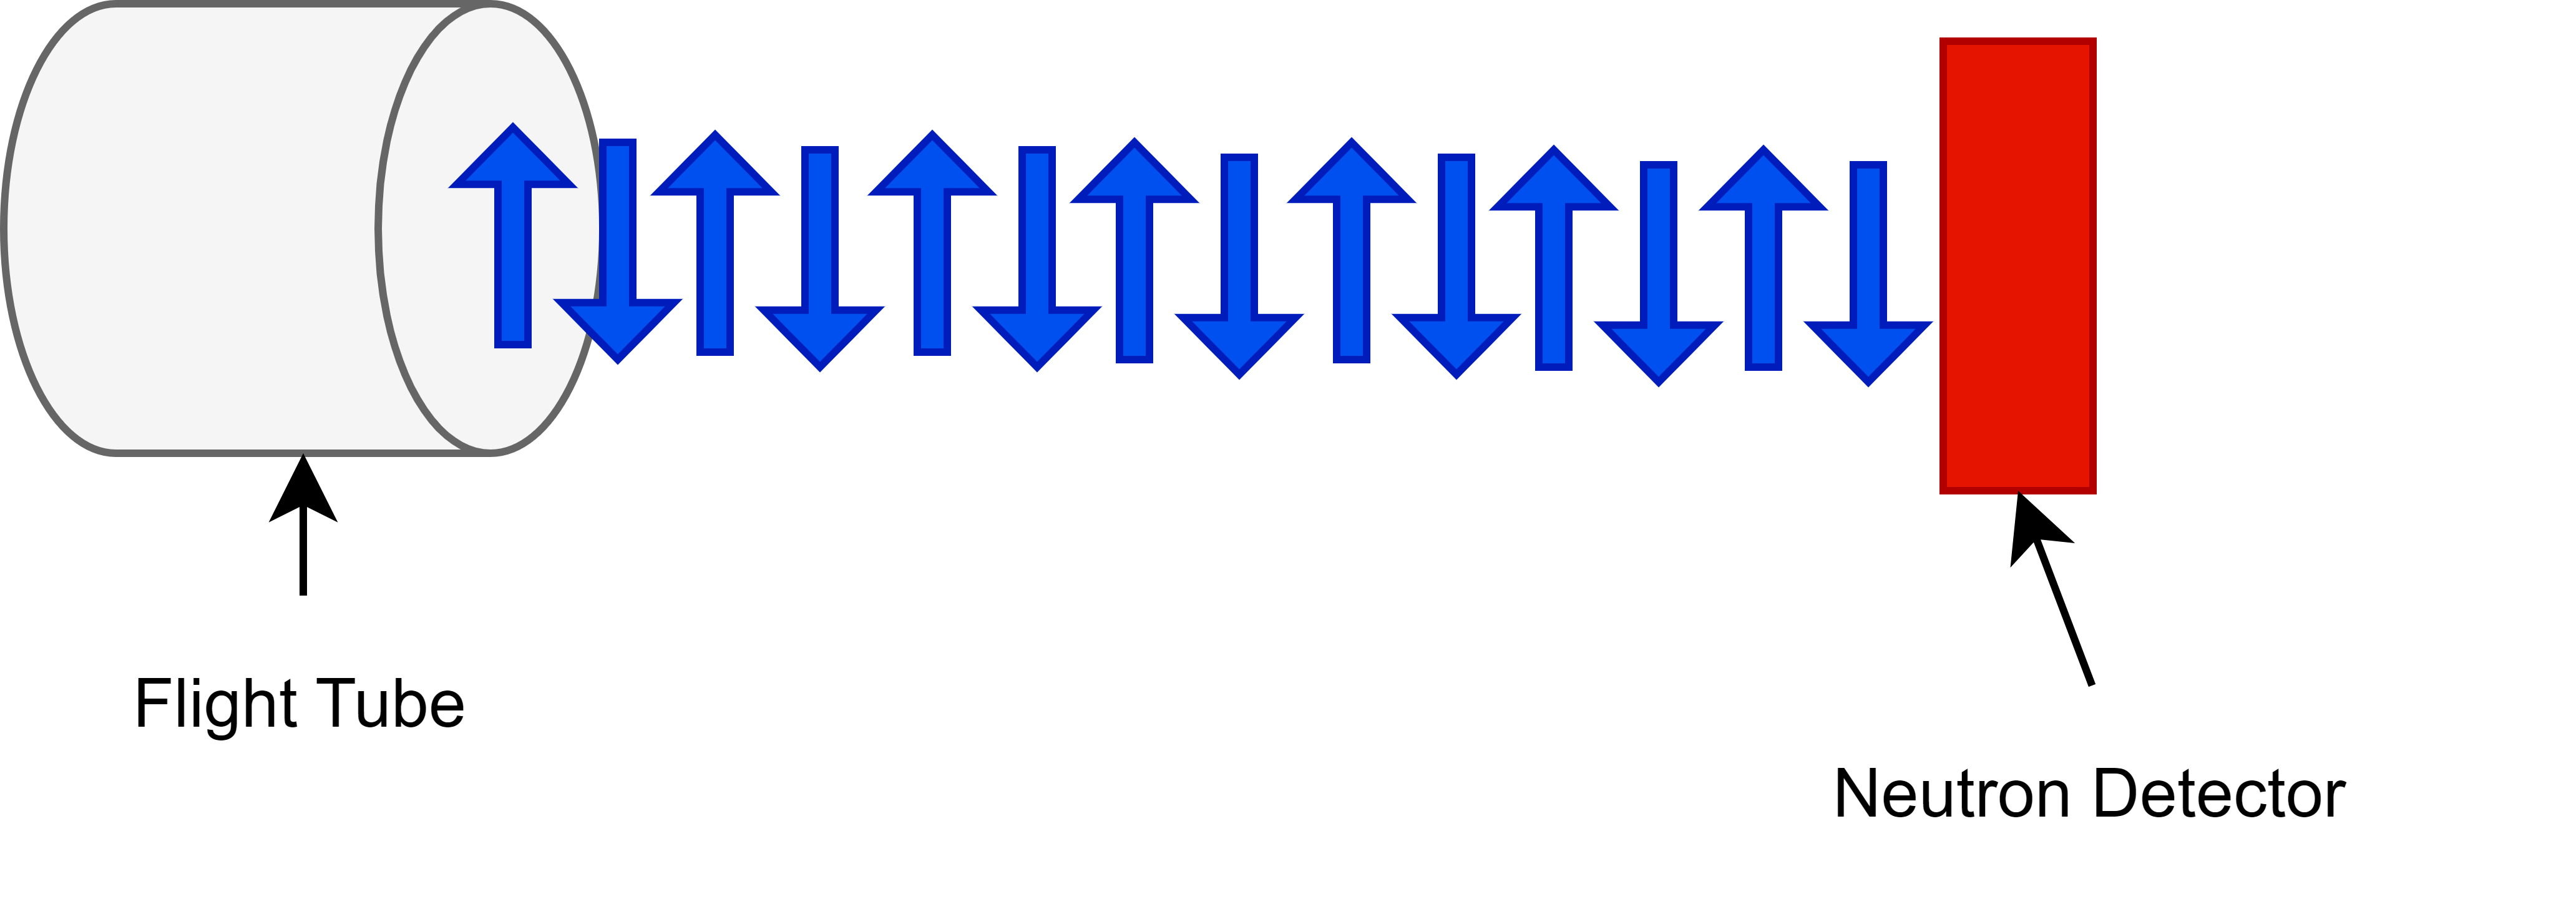
\includegraphics[width=\linewidth, height=4.5cm]{figures/chapter3-figs/unpolbeam_nocell.png}
    \caption{$N_0$}
    \label{fig:directbeam}
    \end{subfigure}
    \hfil
    \begin{subfigure}[b]{0.75\linewidth}
        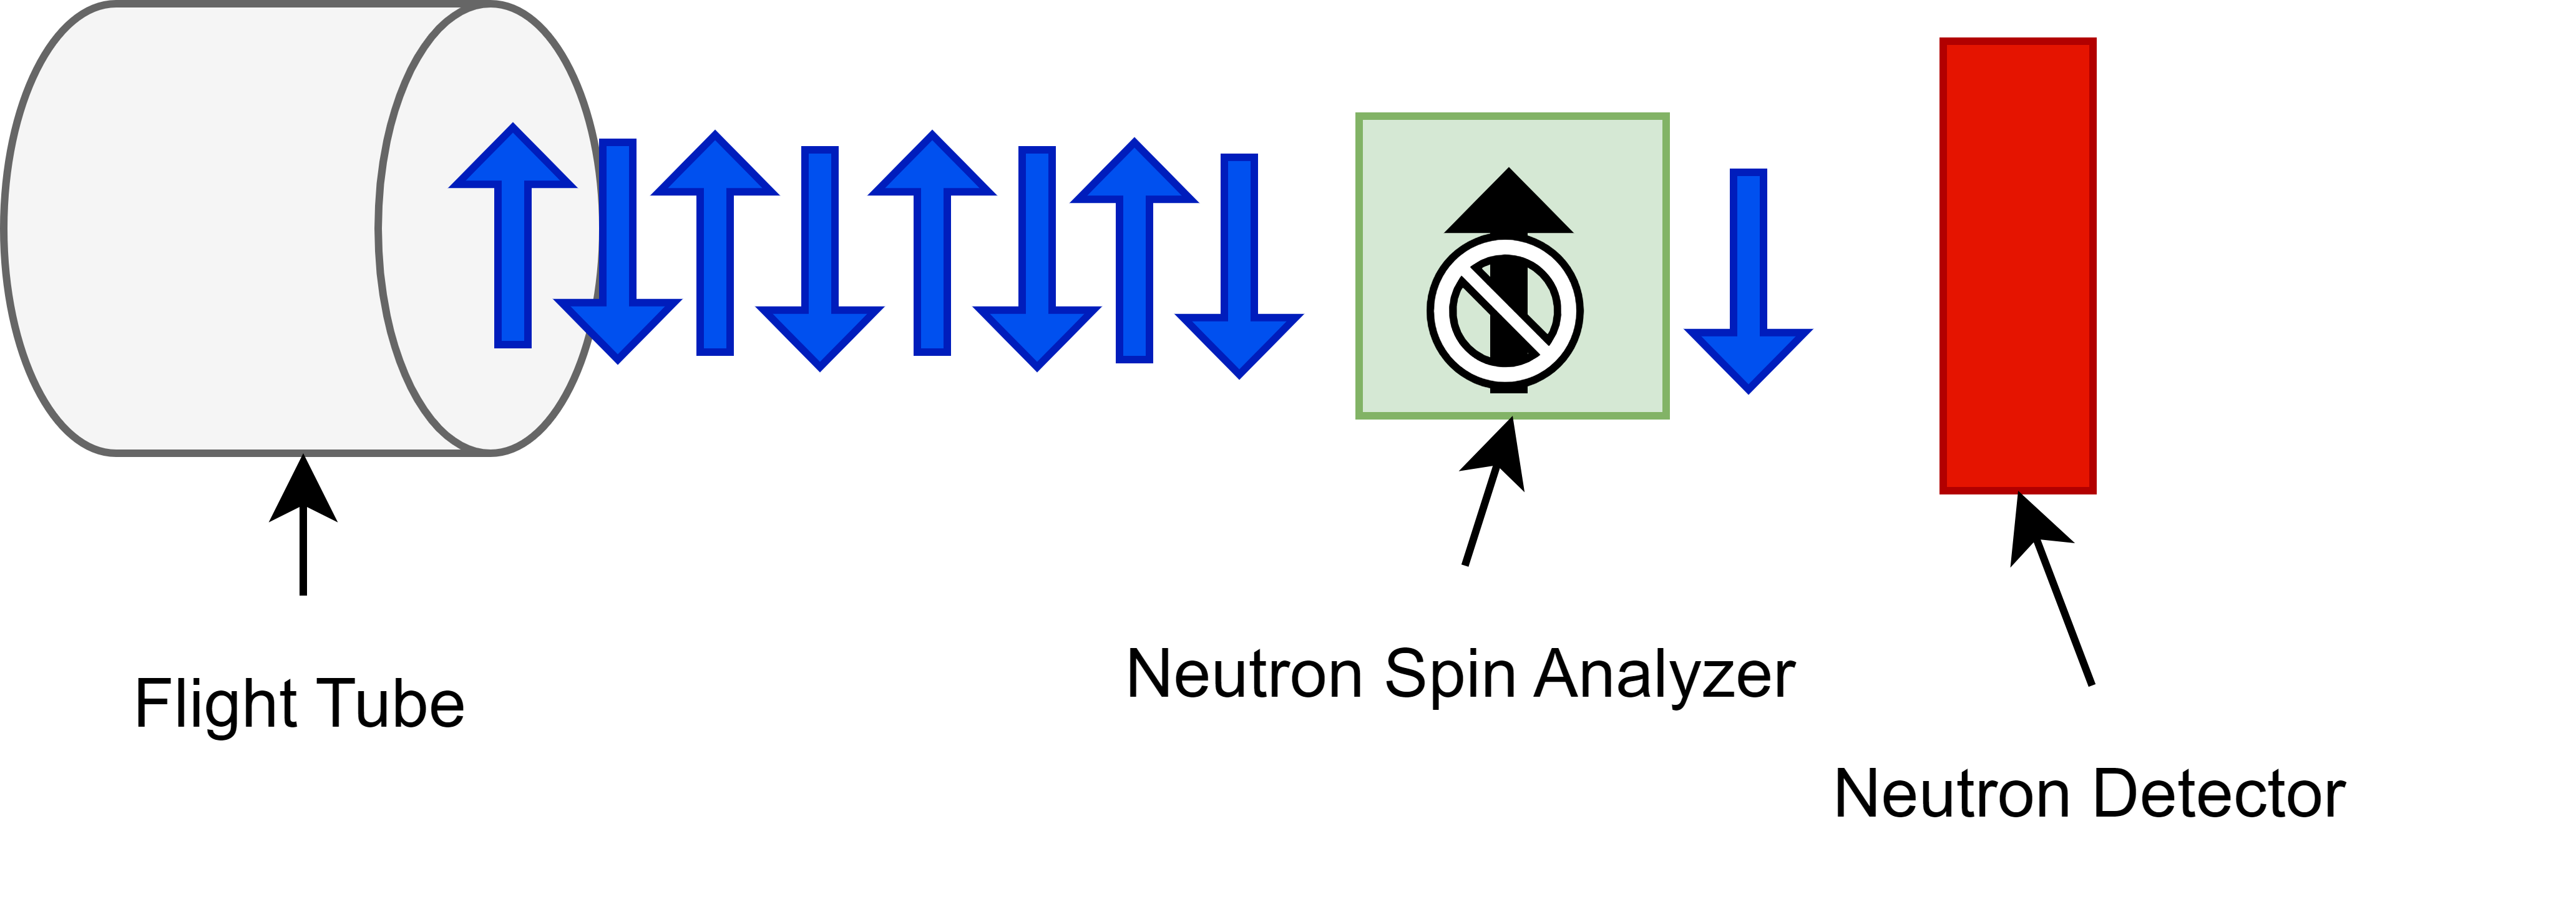
\includegraphics[width=\linewidth, height=4.5cm]{figures/chapter3-figs/unpolbeam_unpolcell.png}
    \caption{$T_{unpol}$}
    \label{fig:unpolcell}
    \end{subfigure}
    \begin{subfigure}[b]{0.75\linewidth}
        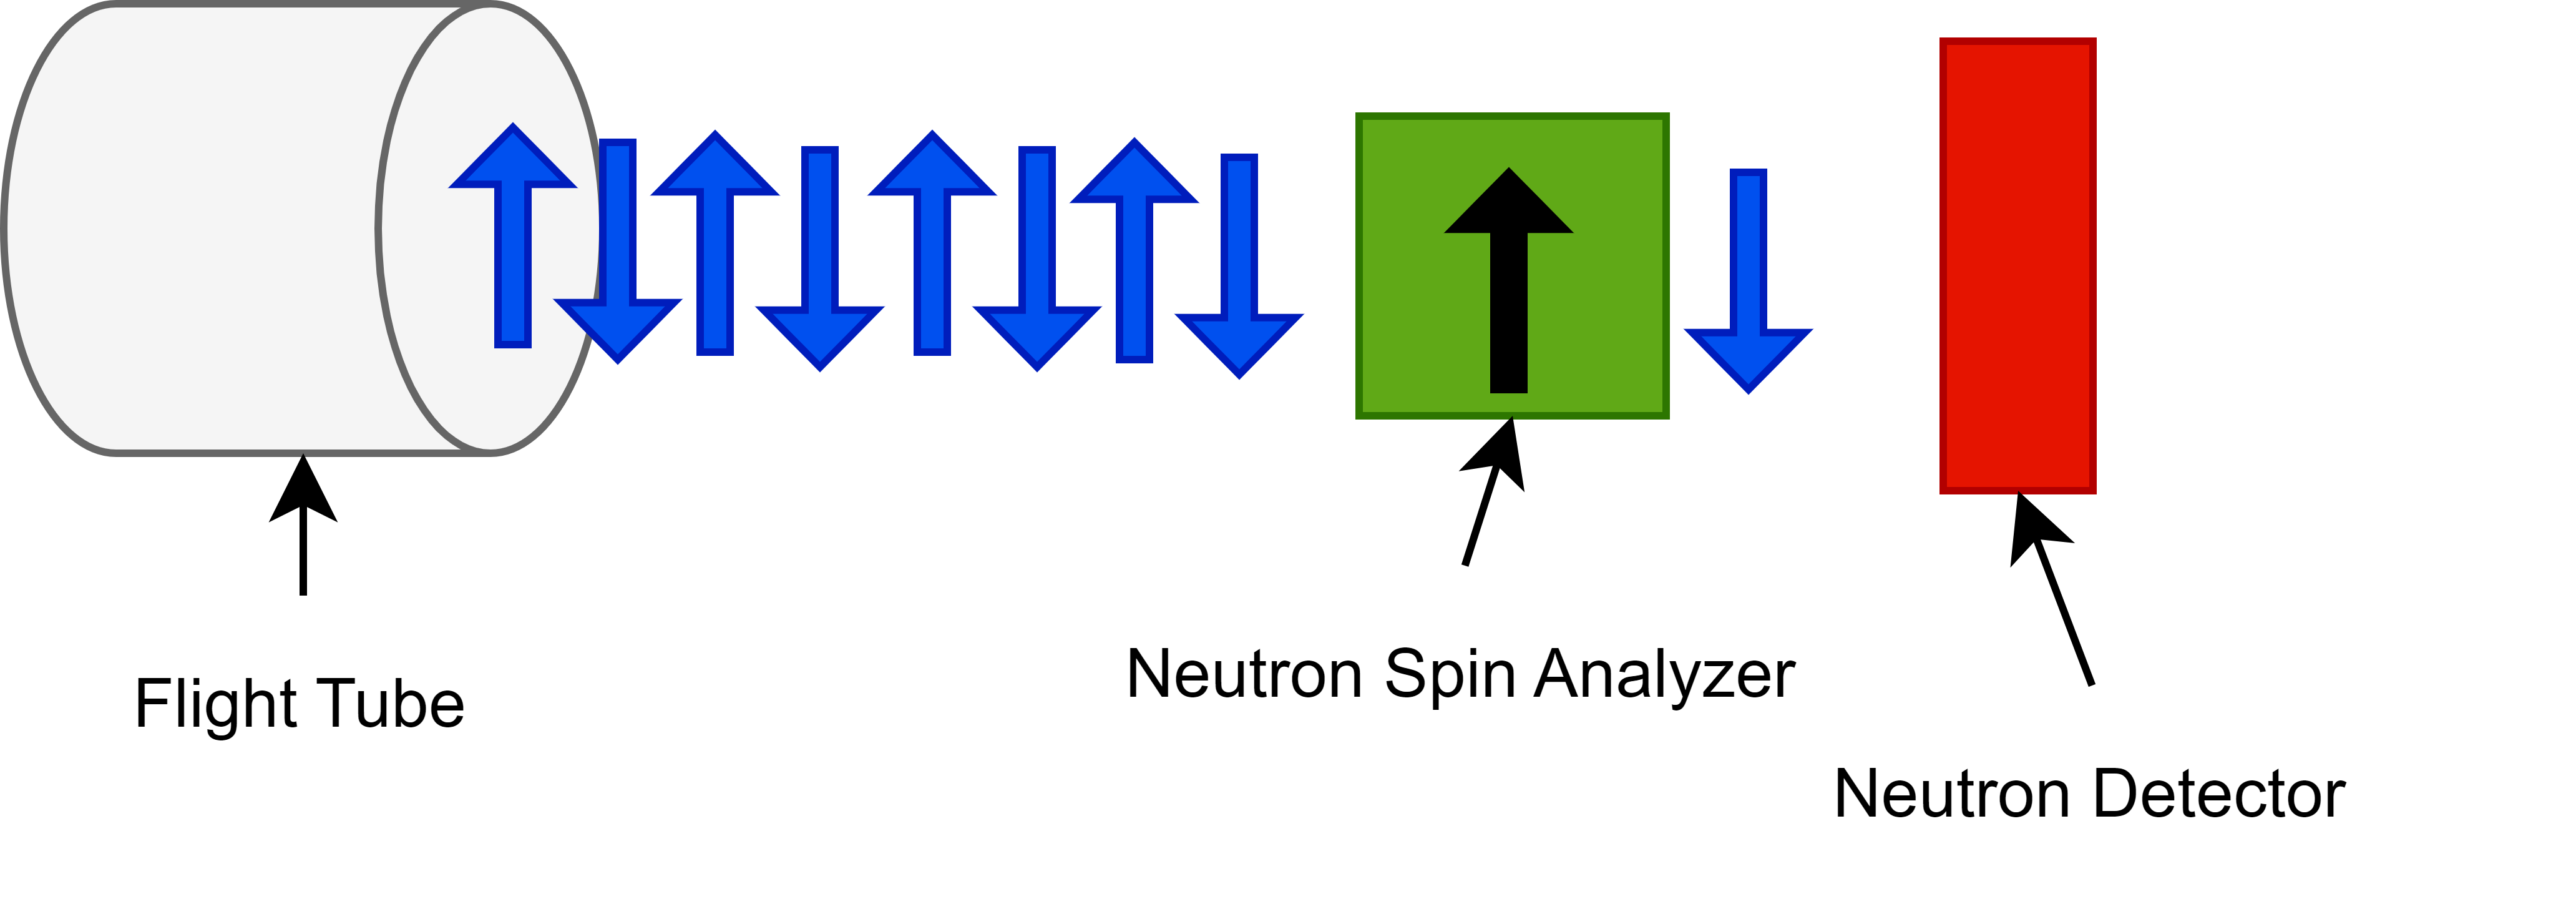
\includegraphics[width=\linewidth, height=4.5cm]{figures/chapter3-figs/unpolbeam_polcell.png}
    \caption{$T_{pol}$}
    \label{fig:polbeam}
    \end{subfigure}
\caption{Transmission of unpolarized neutrons through $^3$He cell for the absolute determination of $^3$He polarization.}
\label{fig:unpol_scheme}
\end{figure}
\clearpage}


\afterpage{
\begin{table}
\centering
\caption{Summary of the transmission measurements of 8.9~\AA\ unpolarized neutron beam through the different configurations of polarized $^3$He cell for the setup shown in \cref{fig:unpol_scheme}.}
\label{tab:unpolbeam}
\begin{tabular}{@{}lccc@{}}
\toprule
State & Beam Polarization State & Analyzer Polarization State & Neutron/s/MW \\ \midrule
$N_0$ & Unpolarized & Not Present & 4489 \\
$T_{unpol}$ & Unpolarized & Unpolarized & 189 \\
$T_{pol}$ & Unpolarized & Polarized & 263 \\ \bottomrule
\end{tabular}
\end{table}
\clearpage}

As part of the in situ system, $^3$He cell Soccer was placed in the unpolarized 8.9~\AA\ monochromatic neutron beamline to characterize the $^3$He polarization as well as the analyzing power. The setup for the transmission of unpolarized 8.9~\AA\ neutrons through the various configuration of $^3$He cell from \cref{eq:Tpol} and \cref{eq:anal_power} is illustrated in \cref{fig:unpol_scheme}. The measurement results are given in \cref{tab:unpolbeam}. Based on these results, the fractional transmission of the unpolarized 8.9~\AA\ neutron beam through an unpolarized Soccer cell, as stated in \cref{eq:Tunpol}, was measured to be:
\begin{equation}
    T_{unpol} = 0.042
\end{equation}
From \cref{eq:Tpol}, the ratio of the transmission of unpolarized neutrons through an polarized Soccer cell to the transmission of unpolarized neutrons through a unpolarized Soccer cell was found to be:
\begin{equation}
    \frac{T_{pol}}{T_{unpol}} = 1.39
\end{equation}
From this, \cref{eq:Tpol} was used to determine the fractional absolute $^3$He polarization as:
\begin{equation}
    P_{He} = 0.27
\end{equation}
and subsequently, \cref{eq:anal_power} was used to extract the fractional analyzing power of Soccer cell as:
\begin{equation}
    P_n^{^3He} = 0.70
\end{equation}
Once absolute $^3$He polarization of the Soccer cell is determined from neutron transmission, it can be used as a reference to calibrate NMR-based relative $^3$He polarization measurements of $^3$He cells with typical accuracy of a few percent \cite{Chen2011}. This method is used extensively in the next chapter, therefore, a more detailed overview and results will be presented there.

%The transmission of unpolarized neutron beam can be approximated from the transmission of a polarized neutron beam as:
%\begin{equation}
 %   \frac{T_{unpol}}{T_{pol}} = \frac{T_0}{ \cfrac{ T_\uparrow + T_\downarrow}{2}}
%\end{equation}
%where $T_0$ is the transmission of polarized neutrons through unpolarized 3He cell, $T_\uparrow$ is the transmission of polarized neutrons through polarized 3He cell and $T_\downarrow$ is the transmission of spin flipped neutrons through a polarized 3He cell. The analyzing power of the 3He from a polarized neutron beam:
%\begin{equation}
%    P_n^{He} = \sqrt{1 - \left(\frac{2T_0}{T_\uparrow + T_\downarrow} \right)^2} = \frac{\sqrt{\left(R_\uparrow + R_\downarrow \right)^2-4}}{R_\uparrow + R_\downarrow}
%\end{equation}
%where $R_\uparrow = \frac{T_\uparrow}{T_0} $  and  $ R_\downarrow = \frac{T_\downarrow}{T_0} $.

%However, the total analyzing power of the polarizer and analyzer is:
%\begin{equation}
%    \epsilon_{ST} \cdot \epsilon_{SF} \cdot P_{n} \cdot P^{He}_{n} = \frac{R_{\uparrow}-R_{\downarrow}}{R_{\uparrow}+R_{\downarrow}}
%\end{equation}
%Cannot separate spin transport efficiency with beam polarization.
%\begin{equation}
%    \epsilon_{ST} \cdot P_{n} \rightarrow P_{n} = \frac {1}{ \epsilon_{SF} \cdot P^{He}_{n} } \left( \frac{R_{\uparrow} - R_{\downarrow}}{R_{\uparrow}+R_{\downarrow}}  \right) =  \frac{R_{\uparrow} - R_{\downarrow}}{ \sqrt{ \epsilon_{SF}^2\left(R_\uparrow + R_\downarrow \right)^2 - 4\epsilon_{SF}^2 }  } 
%\end{equation}
%where $ \epsilon_{SF} = \frac{1}{2} \left(  1 - \frac{R_\downarrow}{R_\uparrow}     \right) $, is the efficiency of the spin flipper used to flip $R_\uparrow$ to $R_\downarrow$.










































